% Options for packages loaded elsewhere
\PassOptionsToPackage{unicode}{hyperref}
\PassOptionsToPackage{hyphens}{url}
%
\documentclass[
  a4paper,
]{article}
\usepackage{amsmath,amssymb}
\usepackage{lmodern}
\usepackage{iftex}
\ifPDFTeX
  \usepackage[T1]{fontenc}
  \usepackage[utf8]{inputenc}
  \usepackage{textcomp} % provide euro and other symbols
\else % if luatex or xetex
  \usepackage{unicode-math}
  \defaultfontfeatures{Scale=MatchLowercase}
  \defaultfontfeatures[\rmfamily]{Ligatures=TeX,Scale=1}
\fi
% Use upquote if available, for straight quotes in verbatim environments
\IfFileExists{upquote.sty}{\usepackage{upquote}}{}
\IfFileExists{microtype.sty}{% use microtype if available
  \usepackage[]{microtype}
  \UseMicrotypeSet[protrusion]{basicmath} % disable protrusion for tt fonts
}{}
\makeatletter
\@ifundefined{KOMAClassName}{% if non-KOMA class
  \IfFileExists{parskip.sty}{%
    \usepackage{parskip}
  }{% else
    \setlength{\parindent}{0pt}
    \setlength{\parskip}{6pt plus 2pt minus 1pt}}
}{% if KOMA class
  \KOMAoptions{parskip=half}}
\makeatother
\usepackage{xcolor}
\usepackage[margin=1in]{geometry}
\usepackage{graphicx}
\makeatletter
\def\maxwidth{\ifdim\Gin@nat@width>\linewidth\linewidth\else\Gin@nat@width\fi}
\def\maxheight{\ifdim\Gin@nat@height>\textheight\textheight\else\Gin@nat@height\fi}
\makeatother
% Scale images if necessary, so that they will not overflow the page
% margins by default, and it is still possible to overwrite the defaults
% using explicit options in \includegraphics[width, height, ...]{}
\setkeys{Gin}{width=\maxwidth,height=\maxheight,keepaspectratio}
% Set default figure placement to htbp
\makeatletter
\def\fps@figure{htbp}
\makeatother
\setlength{\emergencystretch}{3em} % prevent overfull lines
\providecommand{\tightlist}{%
  \setlength{\itemsep}{0pt}\setlength{\parskip}{0pt}}
\setcounter{secnumdepth}{5}
\newlength{\cslhangindent}
\setlength{\cslhangindent}{1.5em}
\newlength{\csllabelwidth}
\setlength{\csllabelwidth}{3em}
\newlength{\cslentryspacingunit} % times entry-spacing
\setlength{\cslentryspacingunit}{\parskip}
\newenvironment{CSLReferences}[2] % #1 hanging-ident, #2 entry spacing
 {% don't indent paragraphs
  \setlength{\parindent}{0pt}
  % turn on hanging indent if param 1 is 1
  \ifodd #1
  \let\oldpar\par
  \def\par{\hangindent=\cslhangindent\oldpar}
  \fi
  % set entry spacing
  \setlength{\parskip}{#2\cslentryspacingunit}
 }%
 {}
\usepackage{calc}
\newcommand{\CSLBlock}[1]{#1\hfill\break}
\newcommand{\CSLLeftMargin}[1]{\parbox[t]{\csllabelwidth}{#1}}
\newcommand{\CSLRightInline}[1]{\parbox[t]{\linewidth - \csllabelwidth}{#1}\break}
\newcommand{\CSLIndent}[1]{\hspace{\cslhangindent}#1}
\usepackage[linesnumbered,lined,boxed,commentsnumbered]{algorithm2e}
\newcommand{\listofalgorithmes}{\tocfile{\listalgorithmcfname}{loa}}
\renewcommand{\contentsname}{Índice}
\renewcommand{\listtablename}{Índice de Tablas}
\renewcommand{\listfigurename}{Índice de Figuras}
\renewcommand{\listalgorithmcfname}{Índice de Algoritmos}
\usepackage{booktabs}
\usepackage{tocbibind}
\usepackage{fancyhdr}
\fancypagestyle{firstpage}{
  \fancyhf{}
  \fancyfoot[C]{\textit{CABA, Argentina. Diciembre 2024}}
}
\usepackage{etoolbox}
\AtBeginDocument{\thispagestyle{firstpage}}
\usepackage{bbm}
\usepackage{pdfpages}
\usepackage{graphicx}
\DeclareUnicodeCharacter{0301}{*************************************}
\usepackage{float}
\floatplacement{figure}{H}
\floatplacement{table}{H}

\usepackage{float}
\ifLuaTeX
  \usepackage{selnolig}  % disable illegal ligatures
\fi
\IfFileExists{bookmark.sty}{\usepackage{bookmark}}{\usepackage{hyperref}}
\IfFileExists{xurl.sty}{\usepackage{xurl}}{} % add URL line breaks if available
\urlstyle{same} % disable monospaced font for URLs
\hypersetup{
  pdftitle={ Cómo encontrar el mejor jugador para tu Equipo de Fútbol},
  pdfauthor={Tomás Glauberman; Ignacio Pardo; Juan Ignacio Silvestri},
  hidelinks,
  pdfcreator={LaTeX via pandoc}}

\title{
\includegraphics[width=5in,height=\textheight]{recursos_pdf/utdt.jpg}\\
Cómo encontrar el mejor jugador para tu Equipo de Fútbol}
\usepackage{etoolbox}
\makeatletter
\providecommand{\subtitle}[1]{% add subtitle to \maketitle
  \apptocmd{\@title}{\par {\large #1 \par}}{}{}
}
\makeatother
\subtitle{Escuela de Negocios - Licenciatura en Tecnología Digital}
\author{Tomás Glauberman\footnote{21F78 \textbar{}
  \href{mailto:tglauberman@mail.utdt.edu}{\nolinkurl{tglauberman@mail.utdt.edu}}} \and Ignacio
Pardo\footnote{21R1160 \textbar{}
  \href{mailto:ipardo@mail.utdt.edu}{\nolinkurl{ipardo@mail.utdt.edu}}} \and Juan
Ignacio Silvestri\footnote{21Q111 \textbar{}
  \href{mailto:jsilvestri@mail.utdt.edu}{\nolinkurl{jsilvestri@mail.utdt.edu}}}}
\date{\textbf{CABA, Argentina. Diciembre 2024}}

\begin{document}
\maketitle
\begin{abstract}
En la última década, el análisis deportivo ha evolucionado hacia una
perspectiva cada vez más matemática y sofisticada. Aplicaciones como el
uso de análisis espacial en Basketball (Goldsberry, 2012) y modelos de
juegos de suma cero en fútbol (Hirotsu y Wright, 2006) son ejemplos
claros de la tendencia creciente en este campo. El béisbol, por mucho
tiempo el deporte preferido para la analítica, ha experimentado una
profunda transformación con la implementación de Sabermetrics (Baumer y
Zimbalist, 2014; Wolf, 2015). La introducción de herramientas analíticas
avanzadas ha producido resultados positivos para muchos equipos, lo que
subraya el valor de estudiar métricas específicas dentro de cada
deporte.

Este desarrollo se centra en el fútbol, un deporte en el cual los
análisis previos se han concentrado, en su mayoría, en predecir
resultados de partidos y mejorar el rendimiento de los equipos. Sin
embargo, este trabajo propone un enfoque diferente al analizar el
impacto de los jugadores sobre la posesión de balón y los disparos del
equipo desde una perspectiva probabilística.

A partir de la métrica PSL propuesta en el paper ``Soccer Networks''
(Huang et al., n.d.), planteamos un proceso para comparar el impacto que
tienen los jugadores sobre la performance del equipo. Logramos formular
una metodología para estudiar la distribución de la performance de un
equipo. Luego, proponemos una serie de métodos y métricas para comparar
el rendimiento de dos formaciones de jugadores. Además, desarrollamos
una forma de representación vectorial (Embeddings) de los jugadores,
llamada Player2Vec, un modelo de Machine Learning tambien basado sobre
el modelo de redes de jugadores planteado en el mismo paper ``Soccer
Networks''. Esto último nos permite desarrollar modelos predictivos
sobre el rendimiento de los jugadores en un equipo. \newpage
\end{abstract}

{
\setcounter{tocdepth}{3}
\tableofcontents
}
\tableofcontents

\newpage

\hypertarget{agradecimientos}{%
\section{\texorpdfstring{\textbf{Agradecimientos}}{Agradecimientos}}\label{agradecimientos}}

Este trabajo no hubiera sido posible sin la ayuda de los profesores
Gustavo Vulcano (Escuela de Negocios, Universidad Torcuato Di Tella) y
Santiago Gallino (The Wharton School, University of Pennsylvania).
Además queremos agradecer a Ignacio Vigilante (TIC - Escuela ORT) y
Tomás Spognardi (Exactas - UBA) por sus contribuciones al modelo de
Player2Vec y al PSL Bayesiano respectivamente.

\textbf{Ignacio Pardo quiere agradecer} a su familia, amigos, colegas y
jefe (Darío Mischener) por su apoyo y acompañamiento durante el
transcurso de su carrera universitaria.

\hypertarget{introducciuxf3n}{%
\section{\texorpdfstring{\textbf{Introducción}}{Introducción}}\label{introducciuxf3n}}

A diferencia de otros deportes como el béisbol o el basketball, el
fútbol ha sido tradicionalmente menos propenso a la aplicación de
técnicas avanzadas de análisis de datos y aprendizaje automático. Sin
embargo, en los últimos años ha habido un crecimiento significativo en
el uso de herramientas analíticas para evaluar el rendimiento de los
jugadores y los equipos.

En la última década el análisis del futbol ha evolucionado hacia una
perspectiva cada vez más matemática y sofisticada. El desarrollo que más
impacto tuvo sin dudas es el de la métrica de Expected Goals
(\textbf{xG}) que permiten evaluar la calidad de las oportunidades de
gol de un equipo. El uso de \textbf{xG} en el análisis de partidos y
jugadores ha permitido una mayor capacidad predictiva y una mejor
comprensión del rendimiento de los equipos.

El trabajo en desarrollo ``Soccer Networks'' (Huang et al., n.d.)
propone un modelo de red de jugadores para calcular la probabilidad de
disparar al arco antes de perder el balón (\textbf{PSL}), lo cual
demuestran tiene alta correlación con el rendimiento del equipo y una
gran importancia al nivel del \textbf{xG}.

Este trabajo profundiza en el análisis de la métrica \textbf{PSL} y
propone un analisis probabilistico sobre las componentes del modelo de
redes de jugadores y su injerencia en el rendimiento de los jugadores y
consecuentemente del equipo. Finalmente, proponemos una metodología para
comparar el rendimiento de jugadores y formaciones de jugadores en base
a la métrica \textbf{PSL}.

\hypertarget{motivaciuxf3n-justificaciuxf3n-del-tema}{%
\section{\texorpdfstring{\textbf{Motivación Justificación del
tema}}{Motivación Justificación del tema}}\label{motivaciuxf3n-justificaciuxf3n-del-tema}}

El fútbol es uno de los deportes más populares y seguidos en todo el
mundo. La capacidad de un equipo para ganar partidos y campeonatos
depende en gran medida de la calidad y el rendimiento de sus jugadores.
En este contexto, la identificación y selección de los mejores jugadores
para un equipo se convierte en una tarea crucial para entrenadores,
directores deportivos y analistas de rendimiento.

\hypertarget{relevancia-acaduxe9mica}{%
\subsection{Relevancia Académica}\label{relevancia-acaduxe9mica}}

Desde una perspectiva académica, el análisis del rendimiento de los
jugadores de fútbol ha sido un área de interés creciente en los últimos
años. La aplicación de técnicas avanzadas de análisis de datos,
aprendizaje automático y modelos probabilísticos ha permitido una
comprensión más profunda del impacto de los jugadores en el rendimiento
del equipo. Algunos ejemplos del estado del arte incluyen el modelo para
maximizar la posesión esperada propuesto en el artículo de Rahimian et
al.~(2023) (Rahimian et al., 2023) y el modelo de redes de jugadores
para calcular la probabilidad de disparar al arco antes de perder el
balón (PSL) presentado en el trabajo de Huang et al.(Huang et al.,
n.d.).

Este trabajo se enmarca en esta línea de investigación, contribuyendo al
desarrollo de nuevas metodologías y herramientas para evaluar y comparar
el rendimiento de los jugadores.

\hypertarget{relevancia-pruxe1ctica}{%
\subsection{Relevancia Práctica}\label{relevancia-pruxe1ctica}}

En el ámbito práctico, la capacidad de identificar a los mejores
jugadores tiene implicaciones directas en la toma de decisiones
estratégicas y operativas de los equipos de fútbol. La correcta
selección de jugadores puede mejorar significativamente el rendimiento
del equipo, aumentar las probabilidades de éxito en competiciones y
optimizar la inversión en fichajes. Además, el uso de modelos avanzados
como Player2Vec y PSL Bayesiano proporciona una ventaja competitiva por
su poder predictivo del rendimiento de los jugadores.

\hypertarget{objetivos-de-proyecto}{%
\section{\texorpdfstring{\textbf{Objetivos de
Proyecto}}{Objetivos de Proyecto}}\label{objetivos-de-proyecto}}

\hypertarget{objetivo-general}{%
\subsection{Objetivo General}\label{objetivo-general}}

El objetivo principal de este proyecto es desarrollar y aplicar modelos
avanzados de análisis de datos y probabilísticos, para mejorar la
evaluación, comparación y selección de jugadores de fútbol. Esto
permitirá a los equipos tomar decisiones más informadas y estratégicas,
optimizando su rendimiento y aumentando sus probabilidades de éxito en
competiciones. Mas concretamente, este trabajo busca responder la
pregunta del titulo ``¿Cómo encontrar al jugador ideal para tu equipo de
fútbol?''.

\hypertarget{objetivos-especuxedficos}{%
\subsection{Objetivos Específicos}\label{objetivos-especuxedficos}}

\begin{enumerate}
\def\labelenumi{\arabic{enumi}.}
\tightlist
\item
  \textbf{Desarrollar un Modelo de Evaluación del Rendimiento de
  Jugadores}:

  \begin{itemize}
  \tightlist
  \item
    Analisar las componentes del modelo de red de jugadores.
  \item
    Explotar el modelo PSL para estimar el impacto de los jugadores en
    el rendimiento del equipo.
  \item
    Crear una representación vectorial de cada jugador para poder
    utilizarlas en modelos predictivos.
  \end{itemize}
\item
  \textbf{Comparar el Rendimiento de Jugadores}:

  \begin{itemize}
  \tightlist
  \item
    Establecer métricas estandarizadas para comparar objetivamente el
    rendimiento de jugadores en diferentes posiciones y roles.
  \item
    Aplicar técnicas de aprendizaje automático y análisis de datos para
    identificar patrones y tendencias en el rendimiento de los
    jugadores.
  \end{itemize}
\item
  \textbf{Optimizar la Selección de Jugadores}:

  \begin{itemize}
  \tightlist
  \item
    Desarrollar un sistema de recomendación para identificar a los
    jugadores que mejor se adaptan a las necesidades y estrategias
    específicas de un equipo.
  \item
    Evaluar la efectividad del sistema de recomendación mediante
    estudios de caso y análisis de datos históricos.
  \end{itemize}
\item
  \textbf{Validar los Modelos}:

  \begin{itemize}
  \tightlist
  \item
    Realizar pruebas y validaciones de los modelos desarrollados
    utilizando datos reales de partidos y jugadores.
  \end{itemize}
\item
  \textbf{Generar Conocimiento y Herramientas para la Comunidad}:

  \begin{itemize}
  \tightlist
  \item
    Documentar y publicar los resultados y metodologías desarrolladas en
    el proyecto.
  \item
    Crear herramientas y recursos accesibles para entrenadores,
    analistas y directores deportivos que deseen aplicar estos modelos
    en sus equipos.
  \end{itemize}
\end{enumerate}

\newpage

\hypertarget{definiciuxf3n-del-problema}{%
\section{\texorpdfstring{\textbf{Definición del
problema}}{Definición del problema}}\label{definiciuxf3n-del-problema}}

A partir de la pregunta de la investigación, se plantea el problema de
encontrar el jugador ideal para un equipo de fútbol. En un comienzo nos
encontramos planteando como definir \emph{performance} de un jugador y
cómo compararla con otros jugadores. Surgió la necesidad de encontrar
una métrica evaluar el impacto de un jugador en el rendimiento de un
equipo y como definir estos agentes. Además es necesario poder
representar concretamente a un Jugdaor \(J\).

\hypertarget{psl-como-muxe9trica-de-performance}{%
\subsection{PSL como métrica de
Performance}\label{psl-como-muxe9trica-de-performance}}

En el paper en proceso \emph{How to Find the Right Player for your
Soccer Team? (Huang et al.)} se plantea la descomposición del Gol
Esperado (\(xG\)) como:

\[
    xG(A) = P(A) \cdot PSL(A) \cdot SA(A)
\]

Donde \(A\) es el equipo, \(P(A)\) es la posesión del balón, \(PSL(A)\)
es la probabilidad patear al arco antes de perder el balón y \(SA(A)\)
es la probabilidad de que un disparo al arco se convierta en gol. A
diferencia de la posesión del balón y la probabilidad de convertir un
disparo en gol, \(PSL(A)\) no es una métrica comúnmente utilizada en el
análisis de fútbol ni existen modelos que la calculen. El paper plantea
un modelo de red de jugadores que permite calcular \(PSL(A)\) para cada
equipo.

\hypertarget{modelo-de-red-de-jugadores}{%
\subsection{Modelo de Red de
Jugadores}\label{modelo-de-red-de-jugadores}}

Utilizando Cadenas de Markov de Tiempo Continuo (CTMC) se puede calcular
la probabilidad de que un equipo pierda el balón antes de patear al
arco. En este modelo de red de jugadores se plantea un modelo de 14
estados: 11 jugadores (\(J_{1} \dots J_{11}\)), Ganancia, Pérdida y
Disparo.

\begin{figure}
  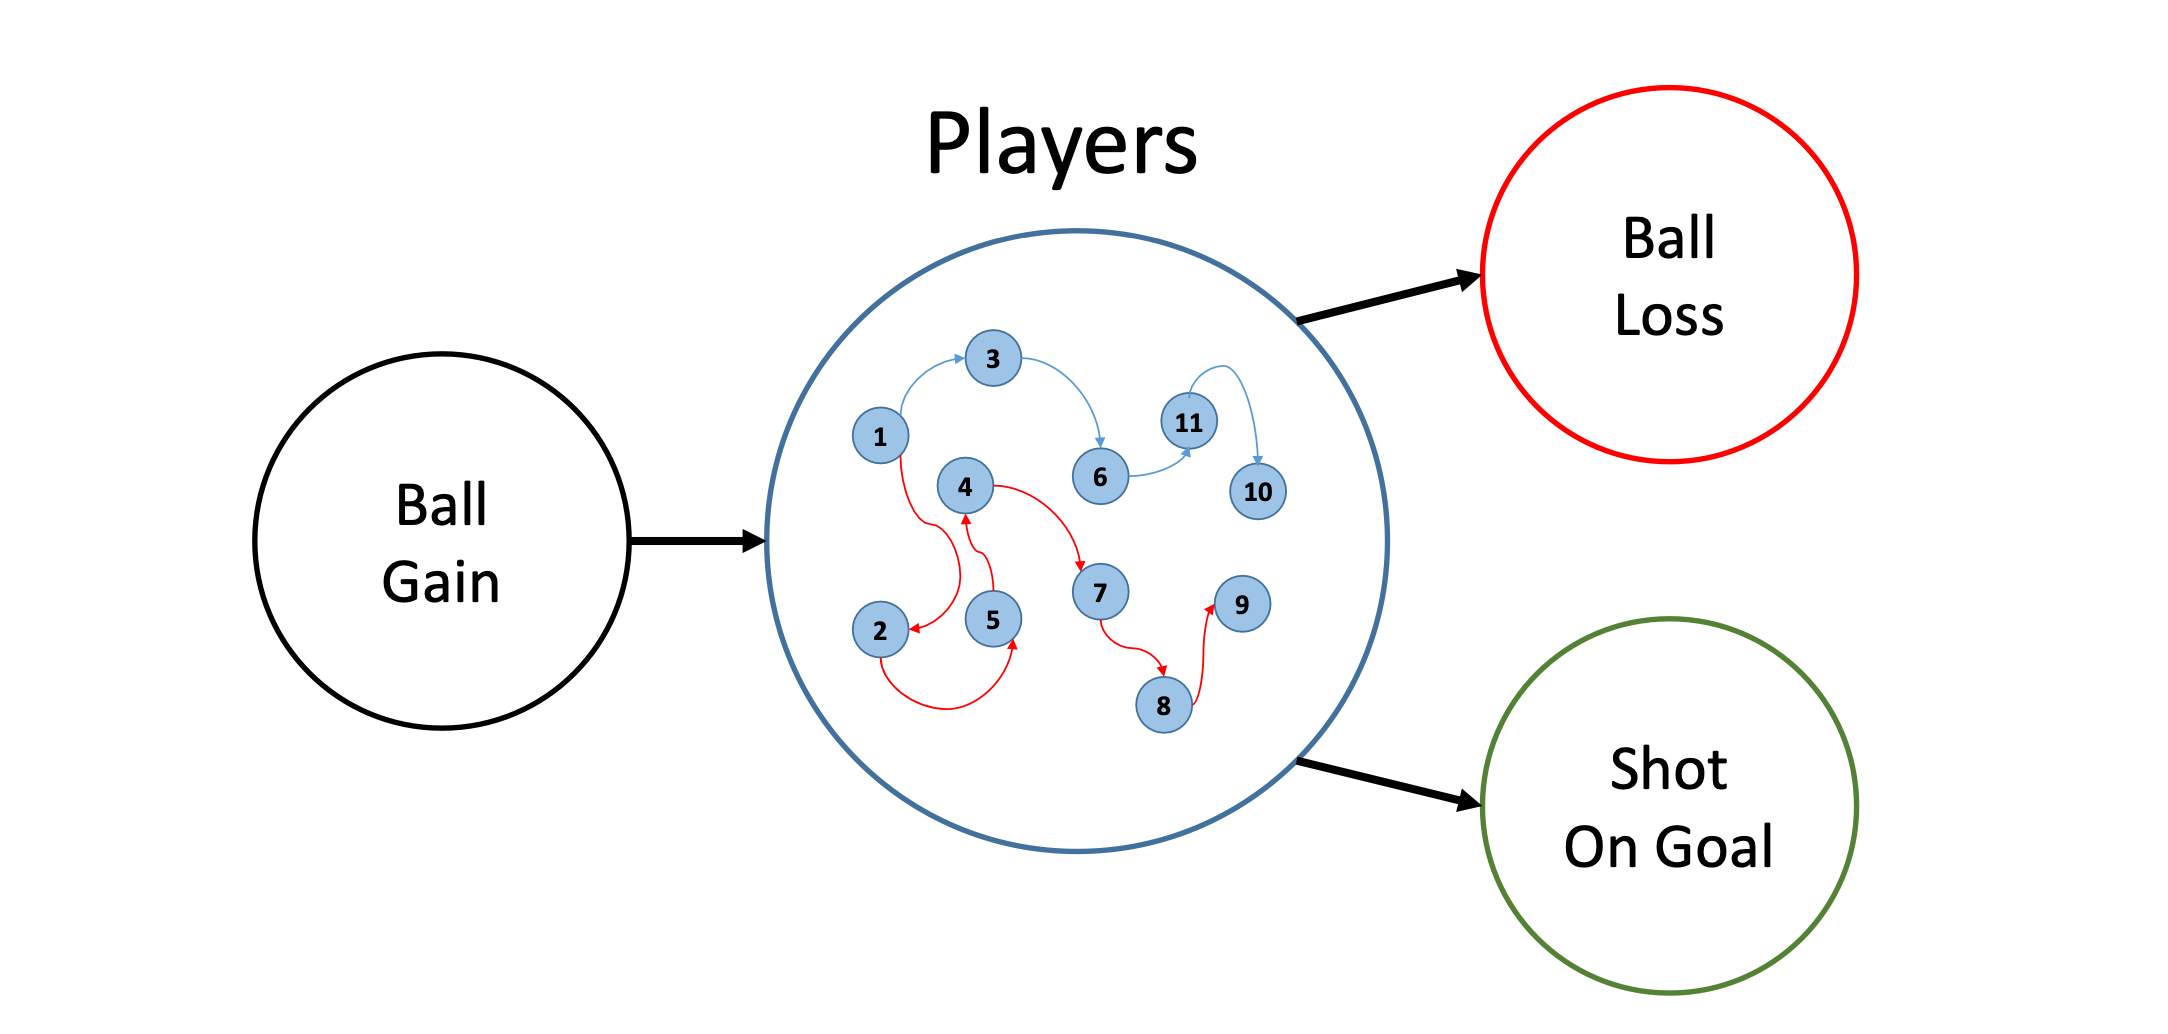
\includegraphics{recursos_pdf/graficos/soccer_network.png}
    \caption{Modelo de Red de Jugadores}
\end{figure}

El grafo presentado en la figura representa el modelo de red de
jugadores. Cada nodo representa un estado y cada arista representa una
transición entre estados. El nodo verde representa el estado de disparo
al arco, el rojo la pérdida del balón y el azul la ganancia del balón
por parte de un jugador. Los ejes entre los nodos se representan con una
matriz de adyasencia \(R\) donde cada valor \(r(U, V)\) representa la
ratio de transición entre los estados \(U\) y \(V\).

\[
    R = \begin{pmatrix}
        0 & r(G, J_{1}) & \dots & r(G, J_{11}) & 0 & 0 \\
        0 & 0 & \dots & r(J_{1}, J_{11}) & r(J_{1}, L) & r(J_{1}, S) \\
        \vdots & \vdots & \ddots & \vdots & \vdots & \vdots \\
        0 & r(J_{11}, J_{1}) & \dots & 0 & r(J_{11}, L) & r(J_{11}, S) \\
        0 & 0 & \dots & 0 & 1 & 0 \\
        0 & 0 & \dots & 0 & 0 & 1 \\
    \end{pmatrix}
\]

A partir de la matriz de ratio de acción sobre tiempo jugado \(R\)
(ganancias, pases a otro jugador, disparos o pérdidas) se puede obtener
la matriz de transición de estados \(Q\) para el CMTC de normalizar las
filas de \(R\):

Para cada par de estados \(U\) y \(V\) se define
\(q(U, V) = \frac{r(U, V)}{\sum_{i=1}^{14} r(U, i)}\)

\[
    Q = \begin{pmatrix}
        0 & q(G, J_{1}) & \dots & q(G, J_{11}) & 0 & 0 \\
        0 & 0 & \dots & q(J_{1}, J_{11}) & q(J_{1}, L) & q(J_{1}, S) \\
        \vdots & \vdots & \ddots & \vdots & \vdots & \vdots \\
        0 & q(J_{11}, J_{1}) & \dots & 0 & q(J_{11}, L) & q(J_{11}, S) \\
        0 & 0 & \dots & 0 & 1 & 0 \\
        0 & 0 & \dots & 0 & 0 & 1 \\
    \end{pmatrix}
\]

Finalmente a partir de la matriz de probabilidades de transición \(Q\)
se puede calcular \(PSL(A)\) como:

\[
    PSL(A) = [1, 0, ..., 0] \cdot (I - T)^{-1} \cdot X \cdot [0, 1]^T
\]

Siendo \(T\) las probabilidades de transición de los estados
transitorios, \(X\) las probabilidades de transición de los estados
transitorios a los estados absorbentes e \(I\) la matriz identidad.

A partir de este modelo en el paper se evaluó para una temporada de la
Premier League (EPL 2012/13) la diferencia entre los PSL de cada equipo
y luego de forma empírica se demuestra como el \(PSL(A)\) tiene alta
correlación positiva con el rendimiento del equipo por sobre el
contrincante. Finalmente hayamos una métrica significativa de
rendimiento de un equipo en la métrica \(PSL\). Sin embargo, da a lugar
a la investigacion de como se puede aplicar esta métrica a nivel de
jugador y como se puede comparar el rendimiento de jugadores en
distintos equipos.

Para evaluar el impacto de un jugador \(J\) se debe, o bien conocer la
probabilidad de transición entre \(J\) y los otros 13 estados (10
jugadores, Ganancia, Pérdida y Disparo) o bien lograr estimar la
probabilidad de transición entre \(J\) y los otros 13 estados.

En estre trabajo se propone un método probabilistico bayesiano para
hayar la Distribución del PSL dada la distribución de probabilidades de
transición entre cada uno de los 11 jugadores y los otros 13 estados.

\hypertarget{modelo-predictivo-de-probabilidades-de-transiciuxf3n}{%
\subsection{Modelo Predictivo de probabilidades de
transición}\label{modelo-predictivo-de-probabilidades-de-transiciuxf3n}}

En un comienzo se planteó desarrollar un modelo predictivo para estimar
las ratios de transición entre los estados. Optamos por buscar predecir
los ratios \(r\) y no las probabilidades de transición \(q\) ya que la
normalización no es igual en cada instancia de \(R\). Mas concretamente
buscamos estimar la función \(f\) que mapea los estados \(U\) y \(V\) a
la ratio de transición \(r(U, V)\).

\[
    \hat{r}(U, V) = f(U, V, \theta)
\]

Comenzamos armando un modelo para predecir unicamente los ratios de
pases \(r(J_i, J_j)\) entre un jugador \(J_i\) y otro jugador \(J_j\).
Lo que correspondereia a los siguientes valores de la matriz \(R\):

\[
    R = \begin{pmatrix}
        0 & r(G, J_1) & \dots & r(G, J_{11}) & 0 & 0 \\
        0 &  \colorbox{yellow}{$0$} & \colorbox{yellow}{$\dots$} & \colorbox{yellow}{$r(J_1, J_{11})$} & r(J_1, L) & r(J_1, S) \\
        \vdots & \colorbox{yellow}{$\vdots$} & \colorbox{yellow}{$\ddots$} & \colorbox{yellow}{$\vdots$} & \vdots & \vdots \\
        0 & \colorbox{yellow}{$r(J_{11}, J_1)$} & \colorbox{yellow}{$\dots$} & \colorbox{yellow}{$0$} & r(J_{11}, L) & r(J_{11}, S) \\
        0 & 0 & \dots & 0 & 1 & 0 \\
        0 & 0 & \dots & 0 & 0 & 1 \\
    \end{pmatrix}
\]

Para poder utilizar un modelo de machine learning tradicional
necestiamos de poder representar a cada jugador \(J\) de forma
vectorial. Armamos un vector de métricas agregadas para un jugador al
momento del partido a predecir. Estas métricas incluyen la cantidad de
pases, disparos, goles, pérdidas, etc. sobre el total de tiempo jugado,
ademas de el equipo en el que juega.

\[
    J = [\text{Passes/90}, \text{Shots/90}, \text{Goals/90}, \text{Losses/90}, \text{Time Played}, \text{Team ID}]
\]

Para el modelo predictivo comenzamos utilizando un modelo de XGBoost
para la regresión pero rápidamente observamos que por la naturelza de
arbol al predecir con la media de las observaciones por hoja las
predicciones resultaban casi discretas, por lo que viramos a explorar un
modelo de regresión lineal para predecir los ratios de pases entre
jugadores.

Para validar elegimos separar de forma temporal los 380 partidos de la
temporada 2012/13 de la EPL: los primeros 269 partidos de entrenamiento;
los últimos 111 de test (\(\mu + 2/3 \sigma\)). Ademas para construir el
dataset, elegimos agarrar parejas de jugadores de los partidos de Train
y removerlos de los mismos para poder en Test predecir ratios de
transición entre jugadores que no se vieron en Train.

Luego de entrenar el modelo, para cada instancia de test obtuvimos la
matriz de ratios de transición \(R\) y calculamos el PSL real, para
luego predecir la matriz de transición \(\hat{R}\) y calcular el PSL
predicho. Finalmente calculamos el coeficiente de correlación de Pearson
entre el PSL real y el PSL predicho.

En el siguiente gráfico podemos observar como a pesar de predecir muy
pobre los ratios de transición al resultar en un coeficiente de
correlación de Pearson entre los \(r(J_i, J_j)\) y los
\(\hat{r}(J_i, J_j)\) de \(0.12\), sin embargo al comparar el PSL real
del PSL calculado a partir de \(\hat{R}\) se obtiene un coeficiente de
correlación de Pearson de \(0.85\).

\begin{figure}
  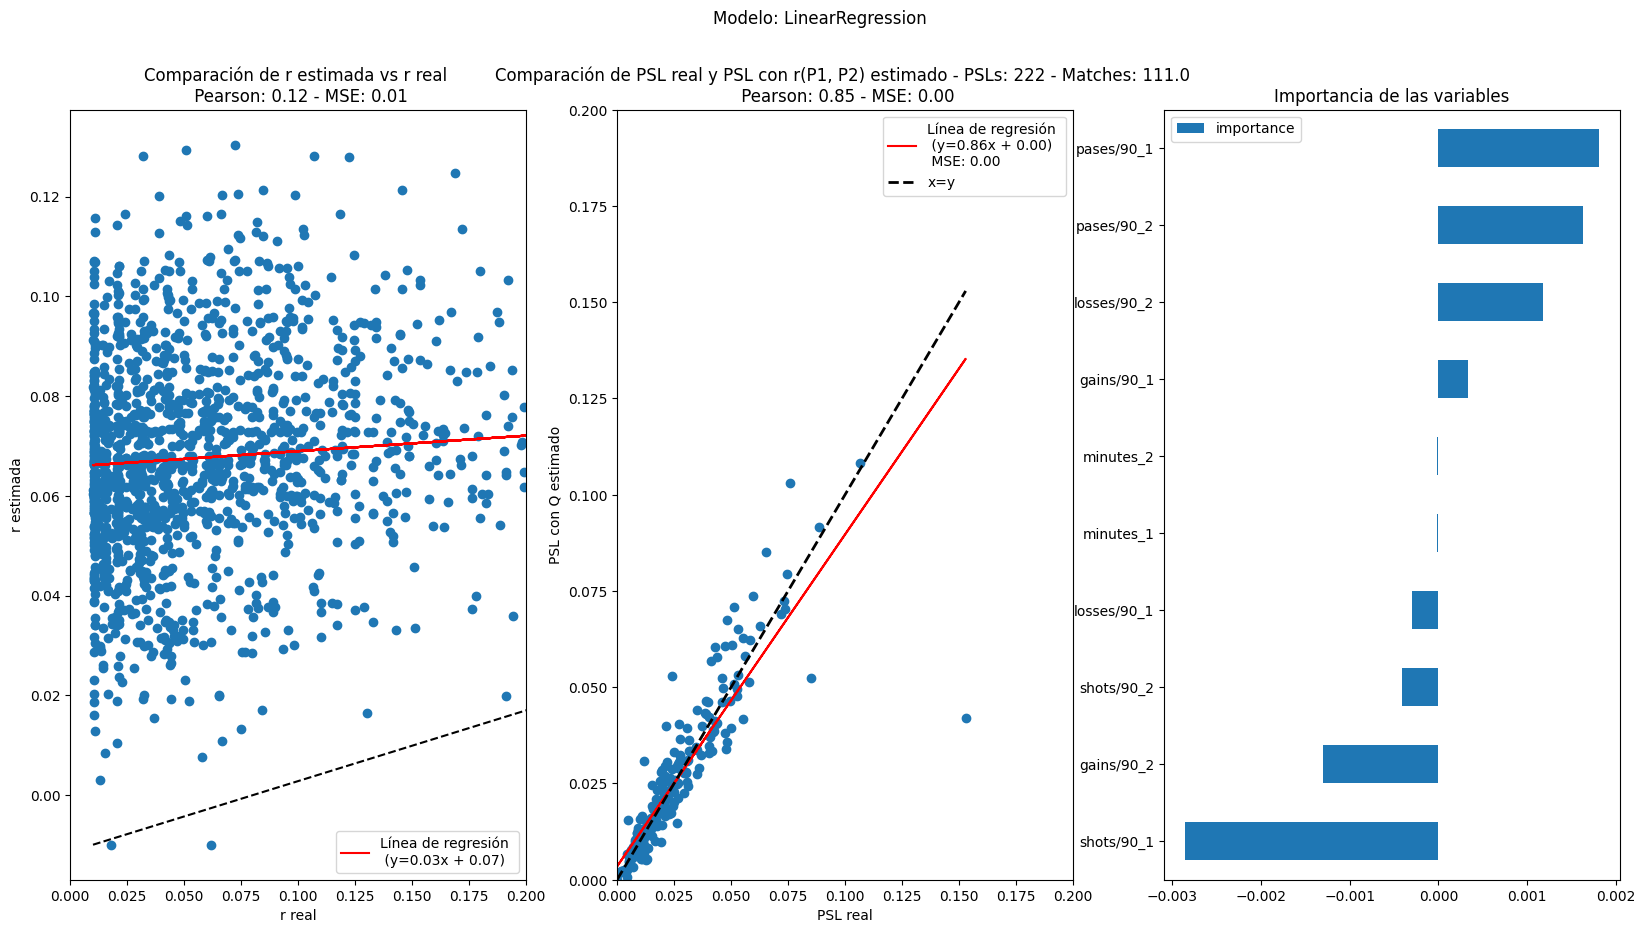
\includegraphics{recursos_pdf/graficos/regresion_lineal_r_p.png}
    \caption{Resultados Modelo de Regresión Lineal}
\end{figure}

El modelo planteado no es capaz de predecir los ratios de transición, y
a pesar de que desarrollamos otros modelos como XGBoost para regressión,
Redes Neuronales y Redes Neuronales Probabilisticas (PNNs) no es posible
predecir los ratios de transición entre los estados a partir de las
métricas de los jugadores. Esto se debe principalmente a la cantidad de
datos y la poca relación entre ellos. Al evaluar como resolver la
predicción de los \(r(J_i, J_j)\) decidimos observar como cada ratio de
transición afecta al PSL.

\hypertarget{test-de-sensibilidad-sobre-psl}{%
\subsection{Test de Sensibilidad sobre
PSL}\label{test-de-sensibilidad-sobre-psl}}

Para entender mejor la relación entre los ratios de transición y el PSL,
se implementó el modelo en una librería de auto-diferenciación (pytorch)
y se obtuvo el gradiente de PSL empíricamente. Esto nos permitió
entender que estados tienen mayor influencia en la métrica que estamos
analizando. Pudimos observar que las transiciones de Jugador a Shot son
las que mas inciden sobre el PSL, seguido por las transiciones entre
jugadores, tal como se observa en la figura.

\begin{figure}
\centering
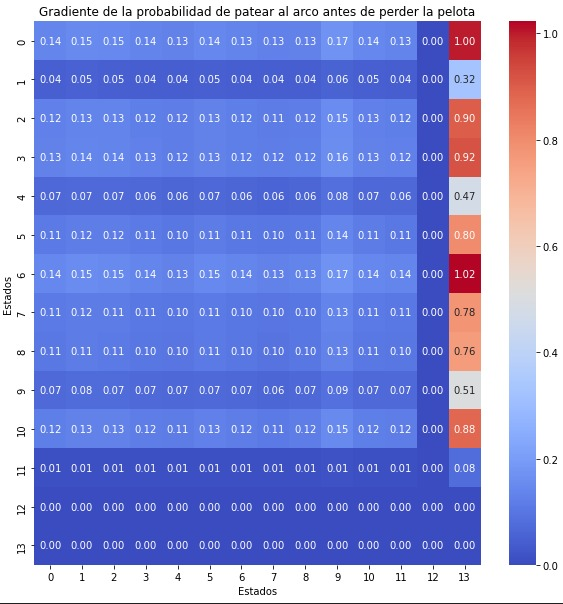
\includegraphics{recursos_pdf/graficos/psl_gradient.jpeg}
\caption{Gradiente del PSL}
\end{figure}

\hypertarget{modelo-predictivo-sobre-rj-s}{%
\subsection{\texorpdfstring{Modelo Predictivo sobre
\(r(J, S)\)}{Modelo Predictivo sobre r(J, S)}}\label{modelo-predictivo-sobre-rj-s}}

Luego de lo observado con el Test de Sensibilidad sobre PSL, decidimos
cambiar el enfoque de la predicción de los ratios de transición entre
jugadores a la predicción de los ratios de transición entre jugadores y
el estado de disparo al arco. Esto se debe a que al observar la matriz
de ratios de transición \(R\) se observa que los ratios de transición
entre jugadores y el estado de disparo al arco son los que más afectan
al PSL.

El nuevo modelo se enfoca en la siguiente sección de la matriz \(R\):

\[
    R = \begin{pmatrix}
        0 & r(G, J_{1}) & \dots & r(G, J_{11}) & 0 & 0 \\
        0 & 0 & \dots & r(J_{1}, J_{11}) & r(J_{1}, L) & \colorbox{yellow}{$r(J_{1}, S)$} \\
        \vdots & \vdots & \ddots & \vdots & \vdots & \colorbox{yellow}{$\vdots$} \\
        0 & r(J_{11}, J_{1}) & \dots & 0 & r(J_{11}, L) & \colorbox{yellow}{$r(J_{11}, S)$} \\
        0 & 0 & \dots & 0 & 1 & 0 \\
        0 & 0 & \dots & 0 & 0 & 1 \\
    \end{pmatrix}
\]

Para el vector de los jugadores \(J\) se agregó tambien la posición en
la que juega (Arquero, Defensor, Mediocampista, Delantero)
one-hot-encoded.

Luego se entrenó un modelo de XGBoost para Regresión con el mismo split
de Train y Test. Se logró obtener un mejor resultado sobre la
predicciones de Train en comparación al modelo anterior, sin embargo al
evaluar en Test. Se obtuvo un coeficiente de correlación de Pearson de
\(0.95\) entre los \(r(J_i, S)\) y los \(\hat{r}(J_i, S)\) en Train,
pero de \(0.08\) en Test.

\begin{figure}
  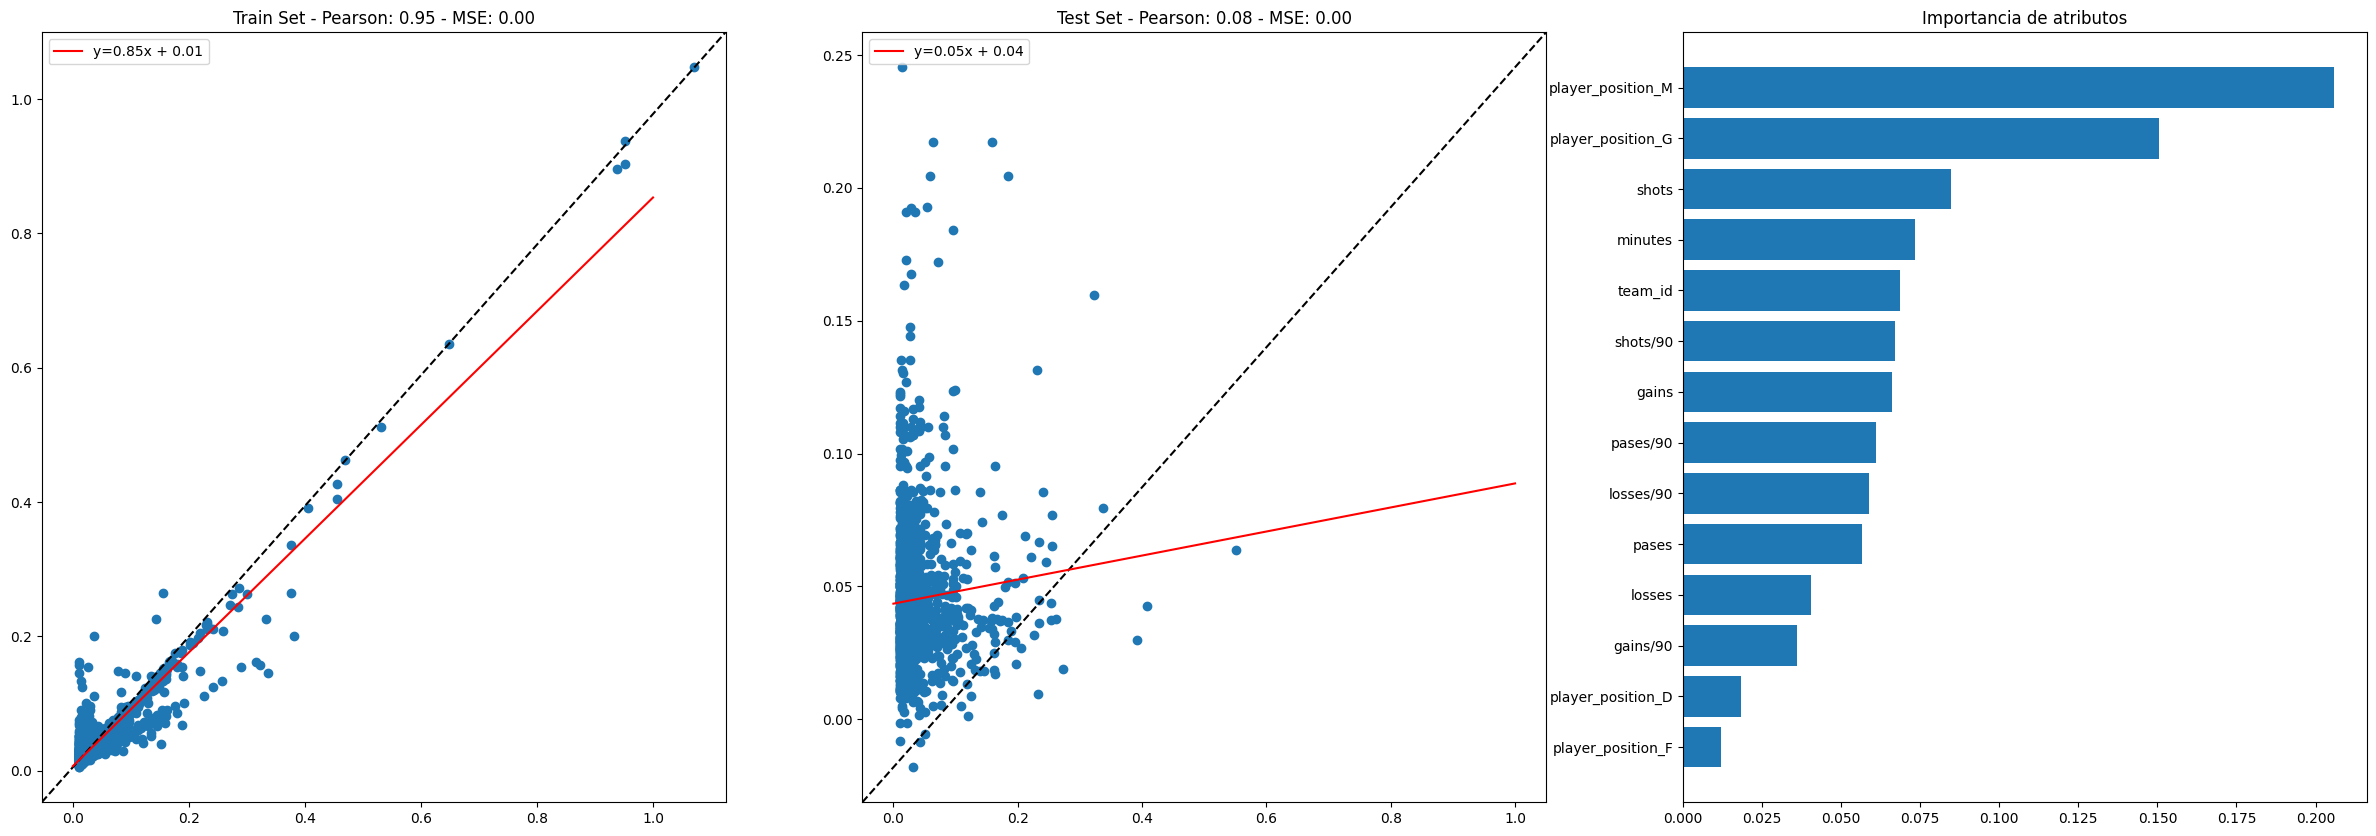
\includegraphics{recursos_pdf/graficos/xgb_shots.png}
    \caption{Resultados Modelo de XGBoost}
\end{figure}

Este resultado junto al del modelo de predicción de ratios de pases nos
llevó a buscar una mejor representación vectorial de los jugadores. En
la sección de Player2Vec se explica el modelo utilizado para obtener un
vector de representación (embedding \(E\)) de cada jugador. Con este
embedding por construimos una red neuronal, el modelo resultante
\(f(E_{J}, \text{partido})\) dado el embedding de los jugadores y el
partido predice los ratios de transición entre jugadores y el estado de
disparo al arco.

\newpage

\hypertarget{analisis-de-las-distribuciones-de-los-rj-s}{%
\section{\texorpdfstring{\textbf{Analisis de las distribuciones de los
\(r(J, S)\)}}{Analisis de las distribuciones de los r(J, S)}}\label{analisis-de-las-distribuciones-de-los-rj-s}}

En un esfuerzo de comprender mejor el modelo de ratios de transición
entre jugadores y el estado de disparo al arco, se decidió analizar las
distribuciones de los \(r(J, S)\) para cada jugador en la temporada
2012/13 de la EPL.

Se observó que las distribuciones de los ratios de transición entre
jugadores y el estado de disparo al arco tienen moda cercana a 0, lo que
indica que la mayoría de los jugadores tienen una baja probabilidad de
disparar al arco antes de perder el balón. En la siguiente figura se
puede observar la distribución de los \(r(J, S)\) para todos los
jugadores de la temporada 2012/13 de la EPL en todos los partidos.

\begin{figure}
  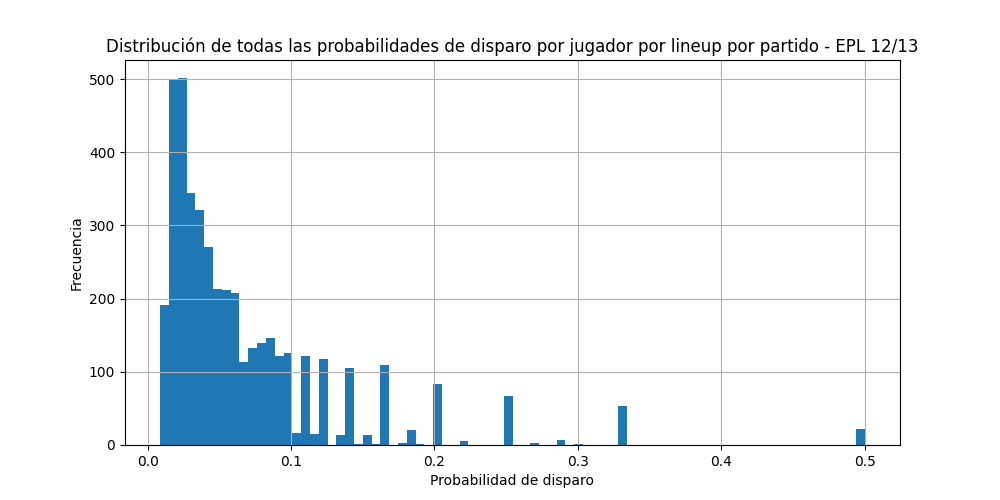
\includegraphics{recursos_pdf/graficos/Probabilidad_de_disparo.png}
    \caption{Distribución de todos los $r(J, S)$}
\end{figure}

Además, se observó que la distribución de los \(r(J, S)\) de cada
jugador no nescesariamente sigue una distribución normal ni similar a la
de otros jugadores.

Para el siguiente analisis se ajustaron las distribuciones de los
\(r(J, S)\) de cada jugador a una distribución de probabilidad beta y se
obtuvieron los parámetros \(\alpha\) y \(\beta\) de cada jugador.

Inicialmente presentamos la distribución de dos jugadores a modo de
ejemplo: \textbf{Sergio Agüero} y \textbf{Robin van Persie}

\begin{figure}
  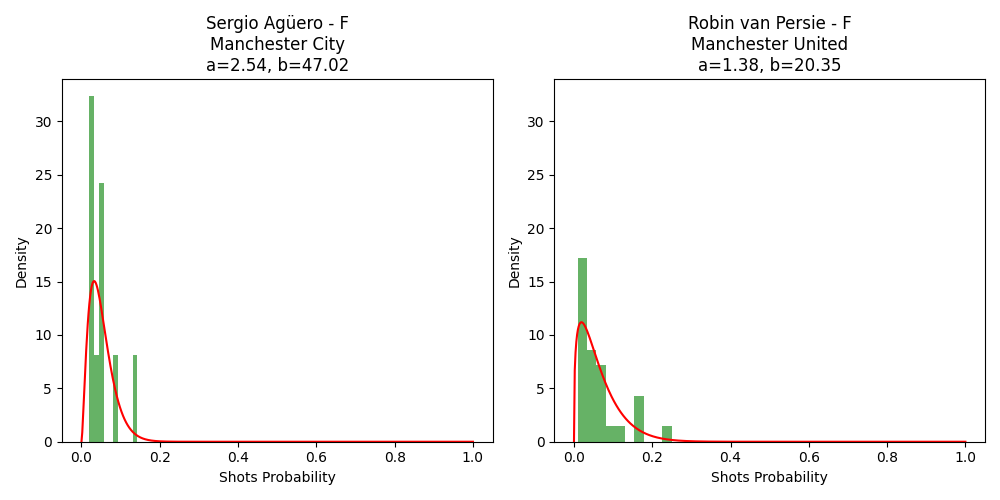
\includegraphics{recursos_pdf/graficos/Sergio_Aguero_Robin_van_Persie_shots_prob_beta_binomial.png}
    \caption{Distribución de los $r(J, S)$ de Sergio Agüero y Robin van Persie}
\end{figure}

Luego se analizó la distribución de los \(r(J, S)\) de los 10 jugadores
con mayor cantidad de disparos, con mayor sesgo y con mayor suma de
disparos a modo de comparación.

\begin{figure}
  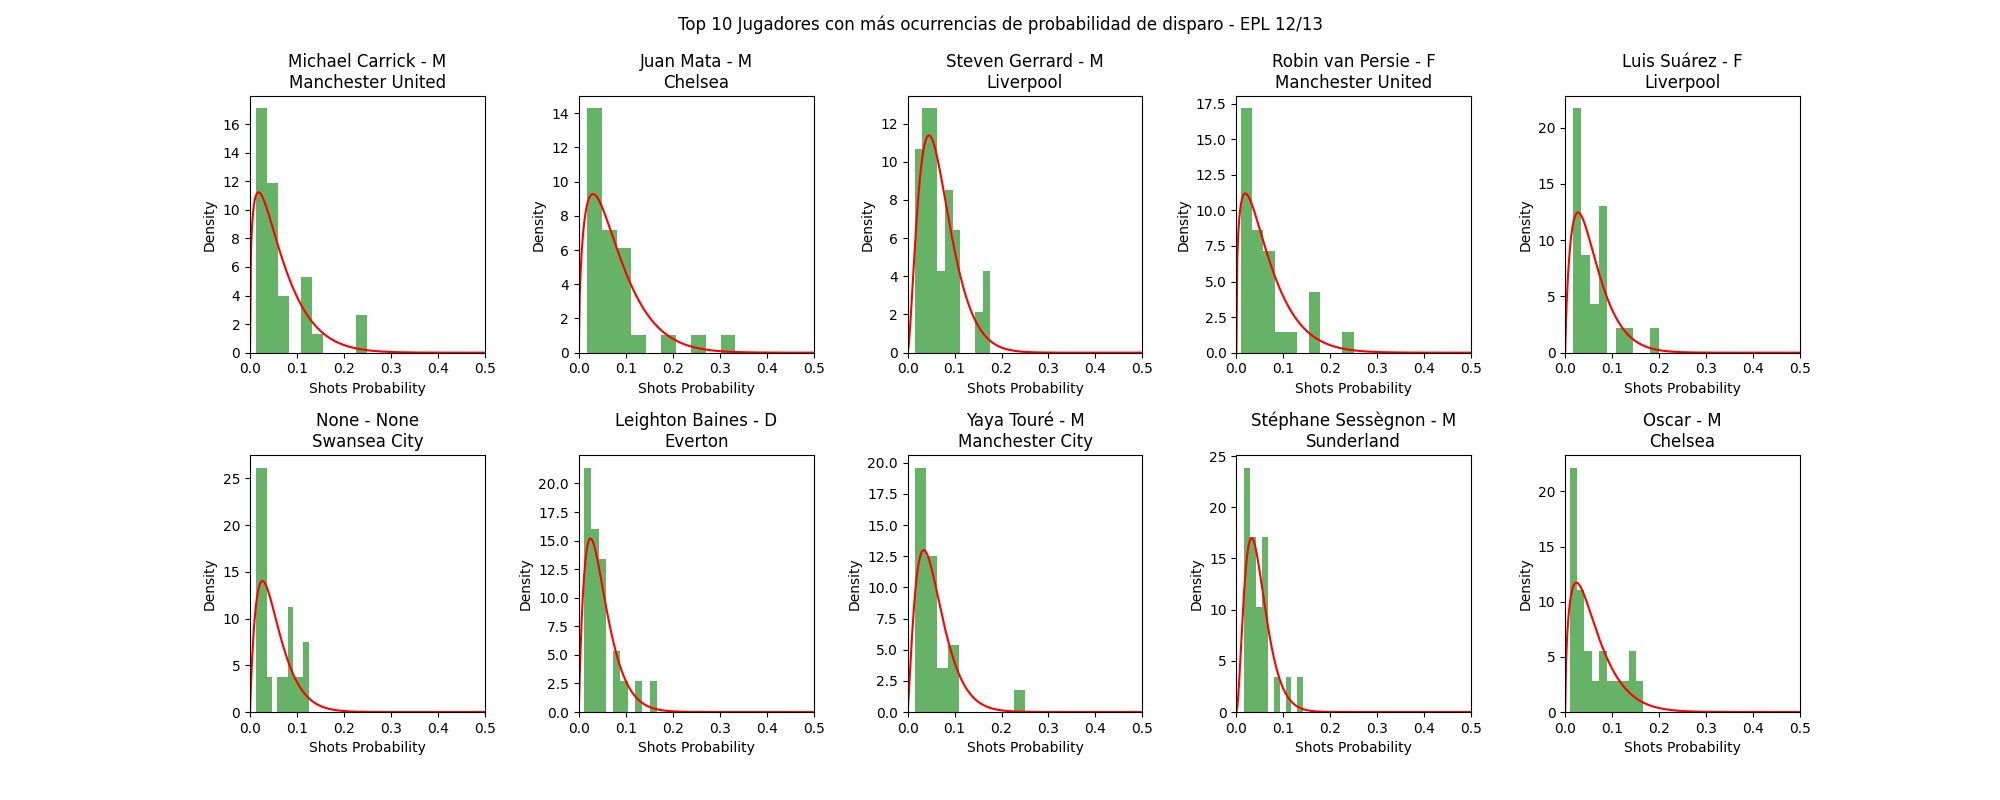
\includegraphics{recursos_pdf/graficos/Top_10_by_counts_players_shots_prob_beta_binomial.png}
    \caption{Distribución de los $r(J, S)$ de los 10 jugadores con mayor cantidad de disparos}
\end{figure}

\begin{figure}
  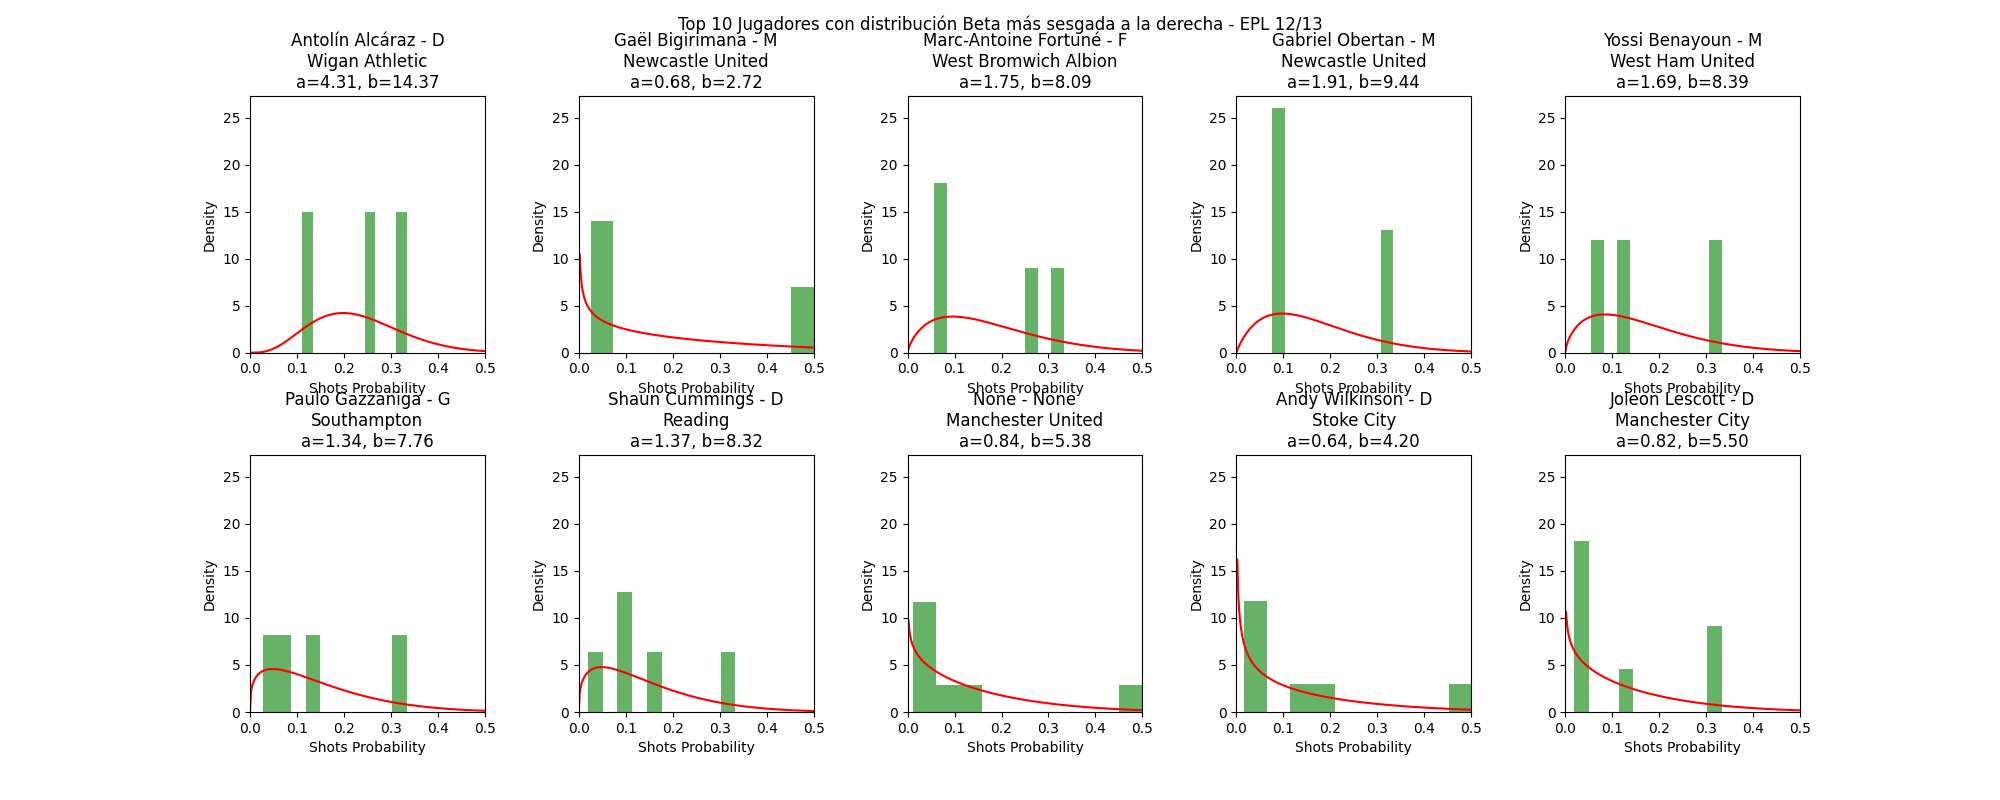
\includegraphics{recursos_pdf/graficos/Top_10_by_skew_players_shots_prob_beta_binomial.png}
    \caption{Distribución de los $r(J, S)$ de los 10 jugadores con mayor sesgo}
\end{figure}

\begin{figure}
  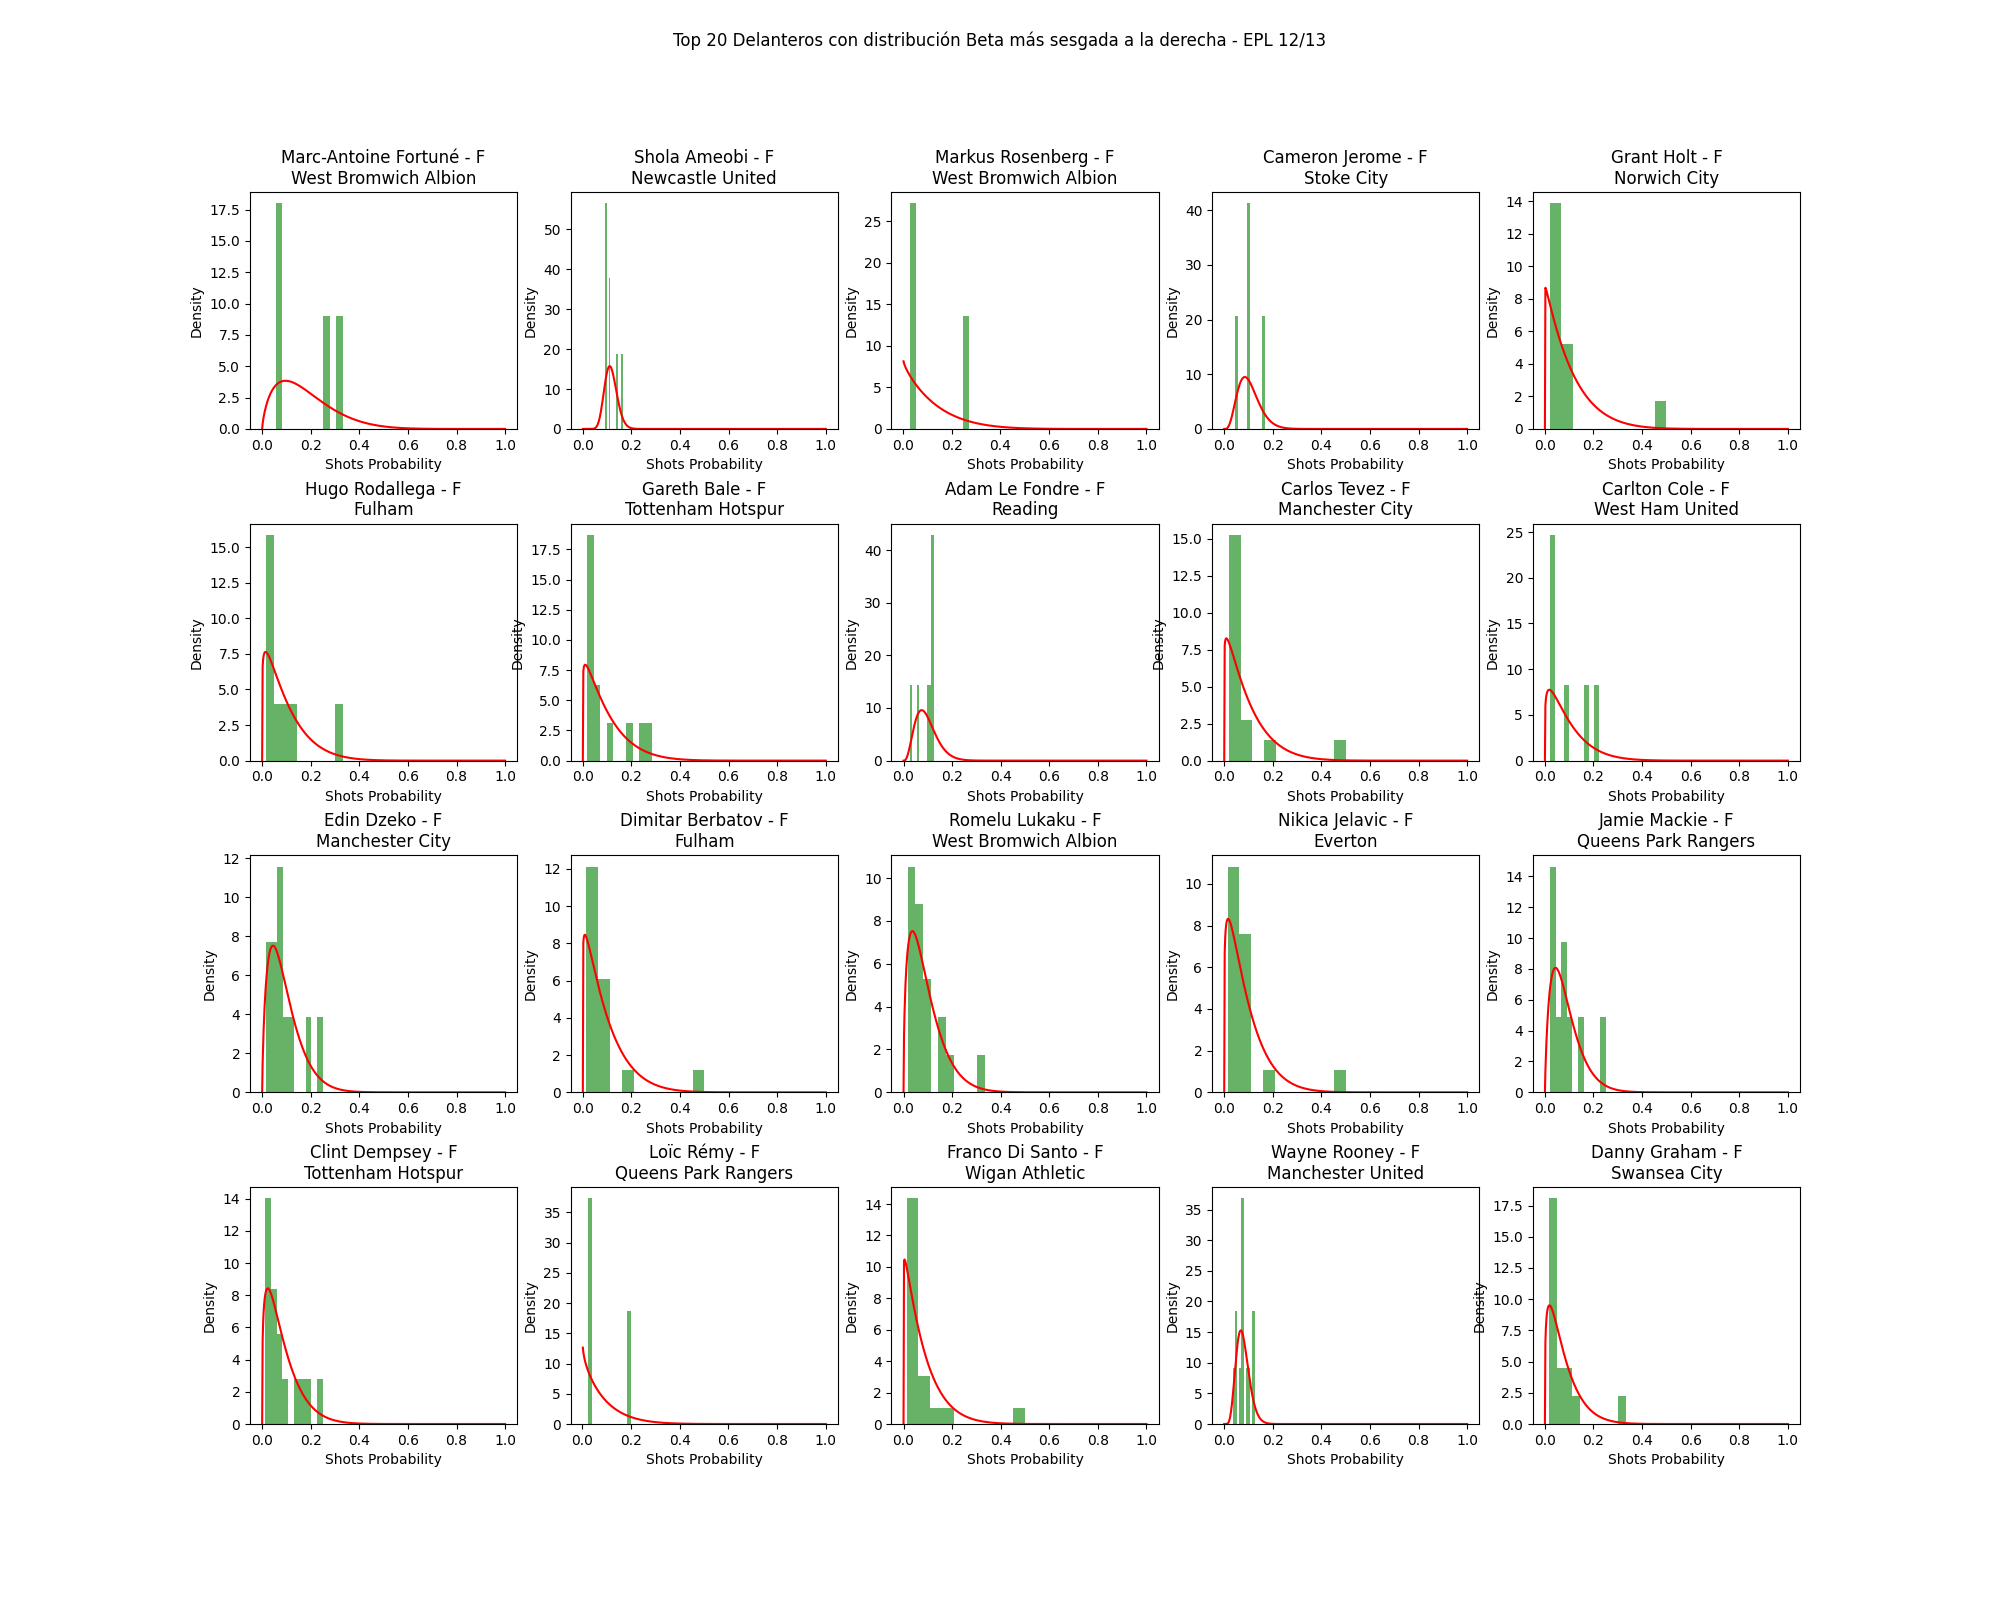
\includegraphics{recursos_pdf/graficos/Top_20_Forwards_by_skew_players_shots_prob_beta_binomial.png}
    \caption{Top 20 Delanteros con distribución Beta más sesgada a la derecha - EPL 12/13}
\end{figure}

\begin{figure}
  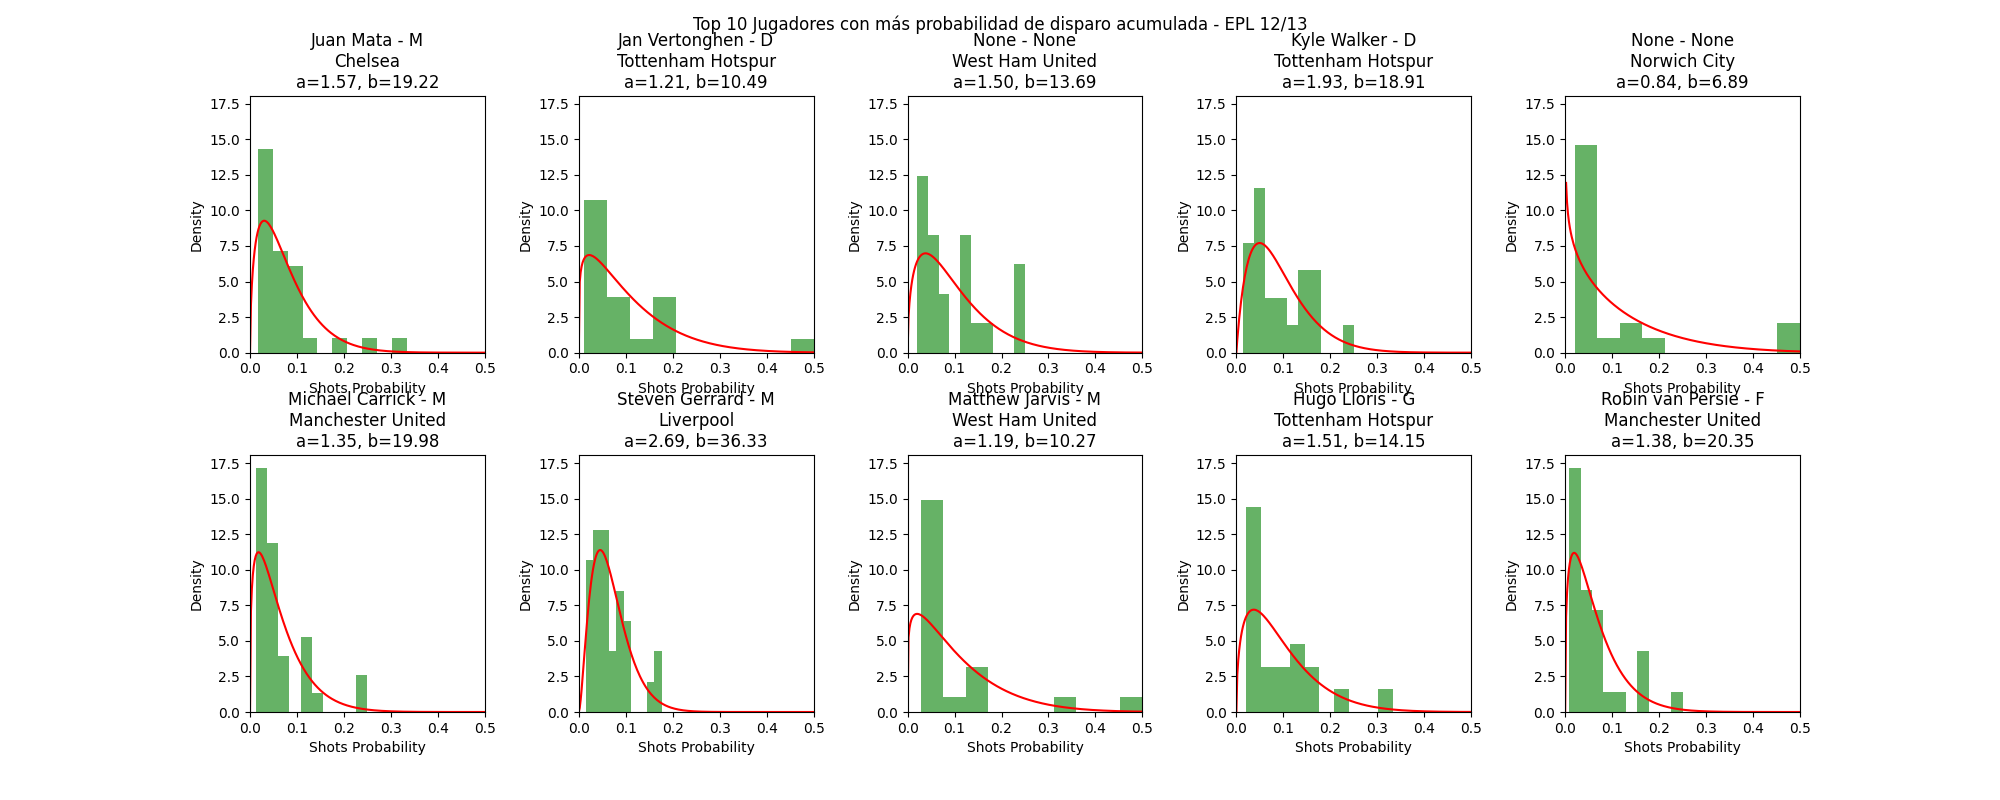
\includegraphics{recursos_pdf/graficos/Top_10_by_sum_players_shots_prob_beta_binomial.png}
    \caption{Distribución de los $r(J, S)$ de los 10 jugadores con mayor suma}
\end{figure}

\hypertarget{comparaciuxf3n-de-las-distribuciones-de-los-rj-s}{%
\subsection{\texorpdfstring{Comparación de las distribuciones de los
\(r(J, S)\)}{Comparación de las distribuciones de los r(J, S)}}\label{comparaciuxf3n-de-las-distribuciones-de-los-rj-s}}

A partir de la distribución ajustada de un jugador, podemos luego hayar
por ejemplo jugadores similares en base a la distribución de los
\(r(J, S)\) utilizando la divergencia de Kullback-Leibler (KL).

En el siguiente gráfico se observa la distribución de los \(r(J, S)\) de
jugadores similares a él en la temporada 2012/13 de la EPL. Además se
presentan solapados en otra figura.

\begin{figure}
  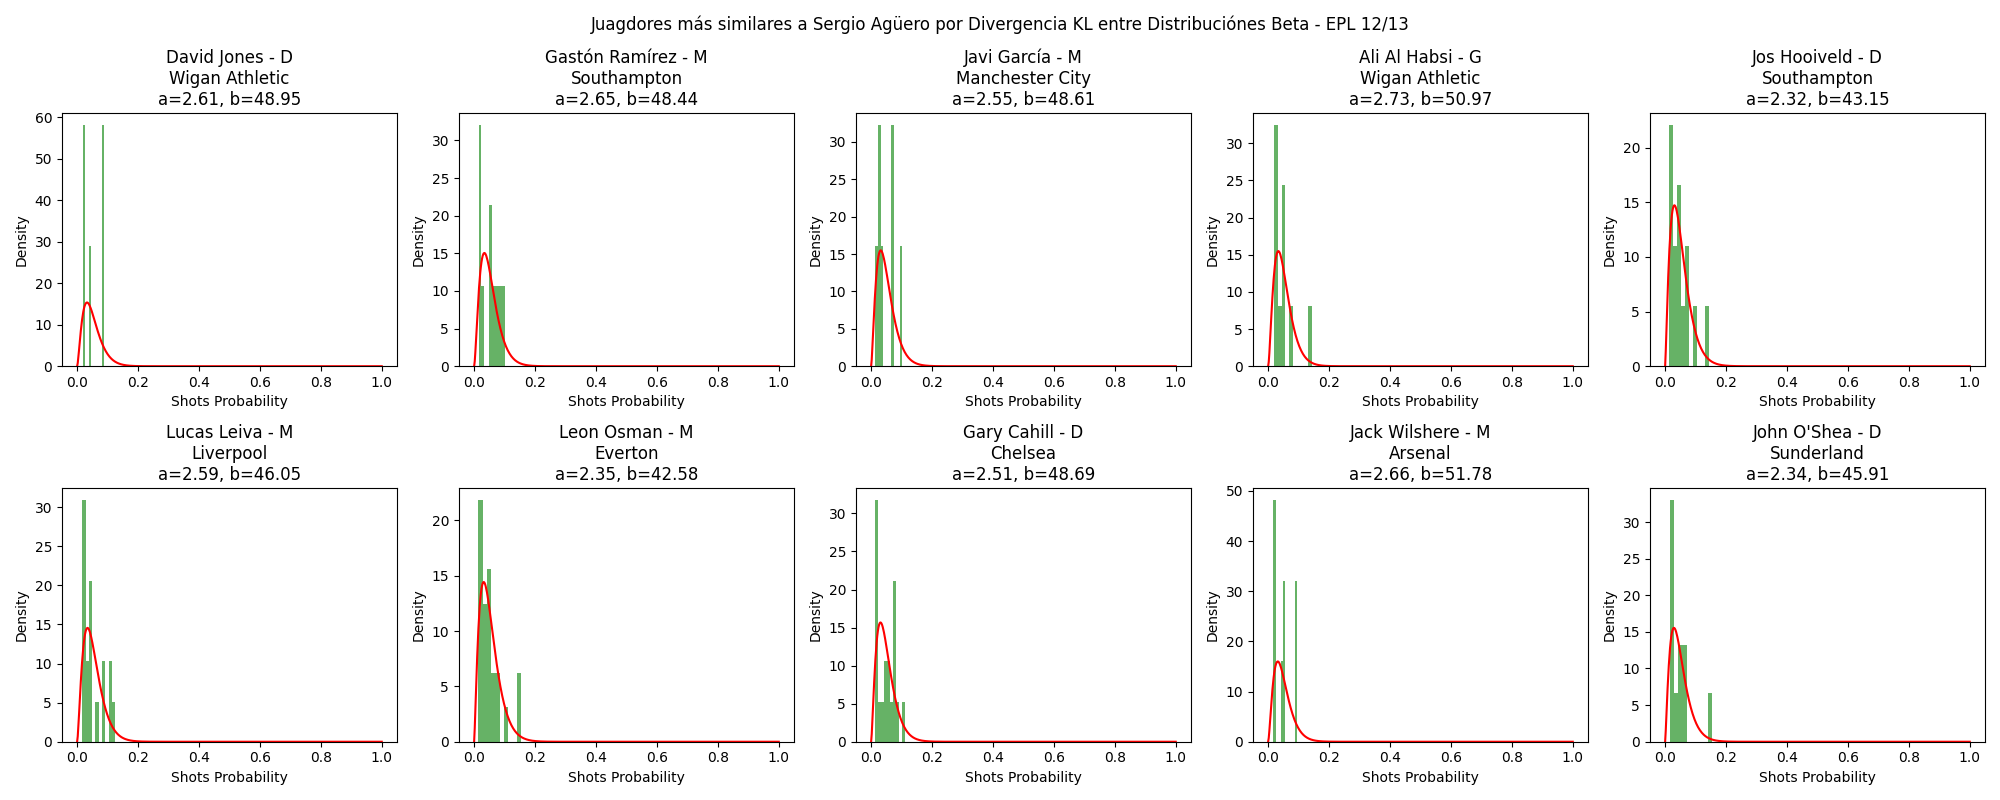
\includegraphics{recursos_pdf/graficos/Similar_to_Sergio_Aguero_shots_prob_beta_binomial.png}
    \caption{Distribución de los $r(J, S)$ de jugadores similares a Sergio Agüero}
\end{figure}

\begin{figure}
  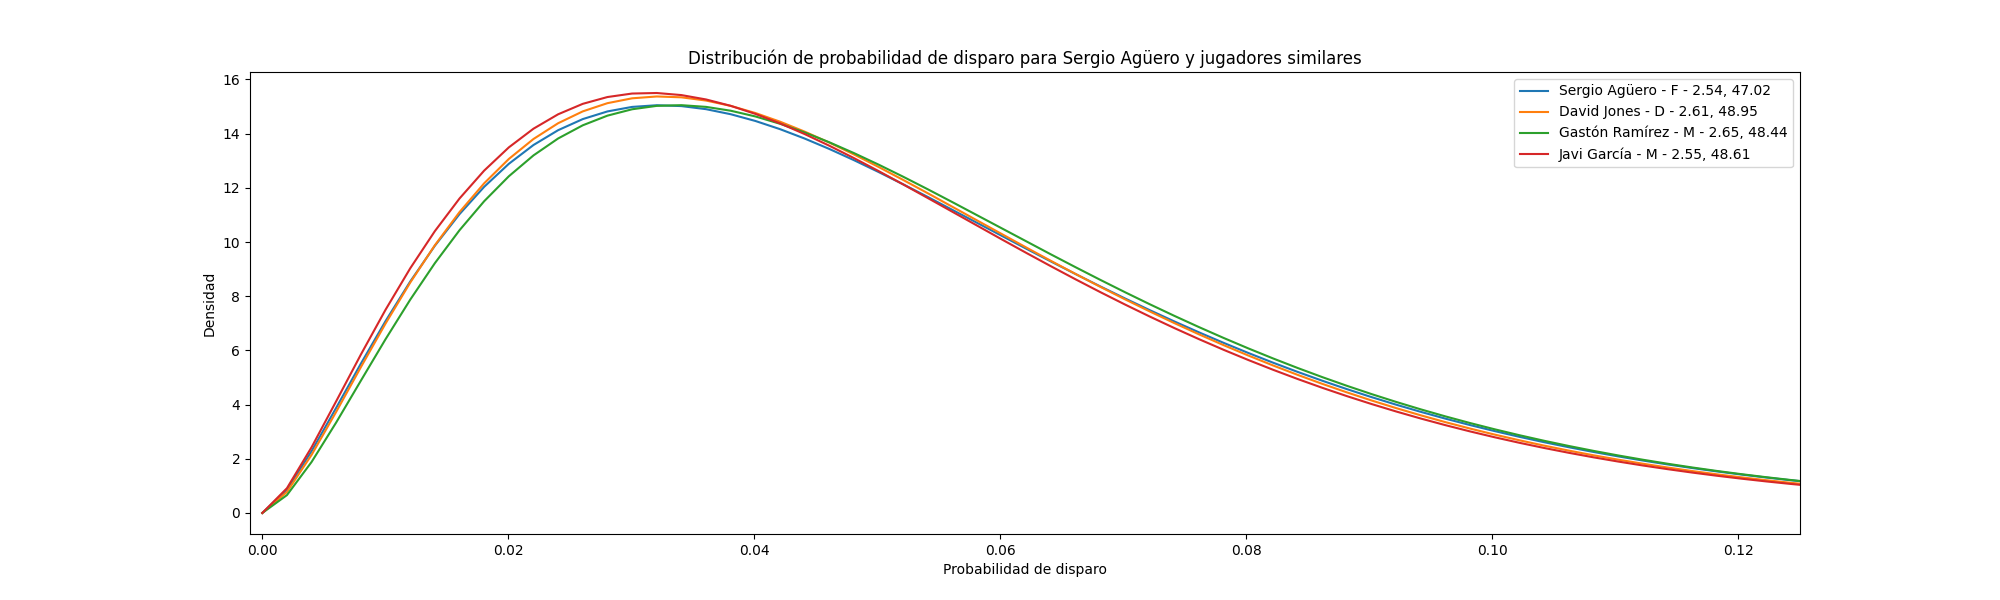
\includegraphics{recursos_pdf/graficos/Sergio_Aguero_and_similar_players_shots_prob_beta_binomial.png}
    \caption{Distribución de los $r(J, S)$ de jugadores similares a Sergio Agüero Superpuestos}
\end{figure}

Finalmente podemos agregar la condición de \emph{misma posición} al
comparar dos jugadores, en el caso de Agüero de Delantero (F por
Forward) y hayar nuevamente jugadores aún mas similares a el.

\begin{figure}
  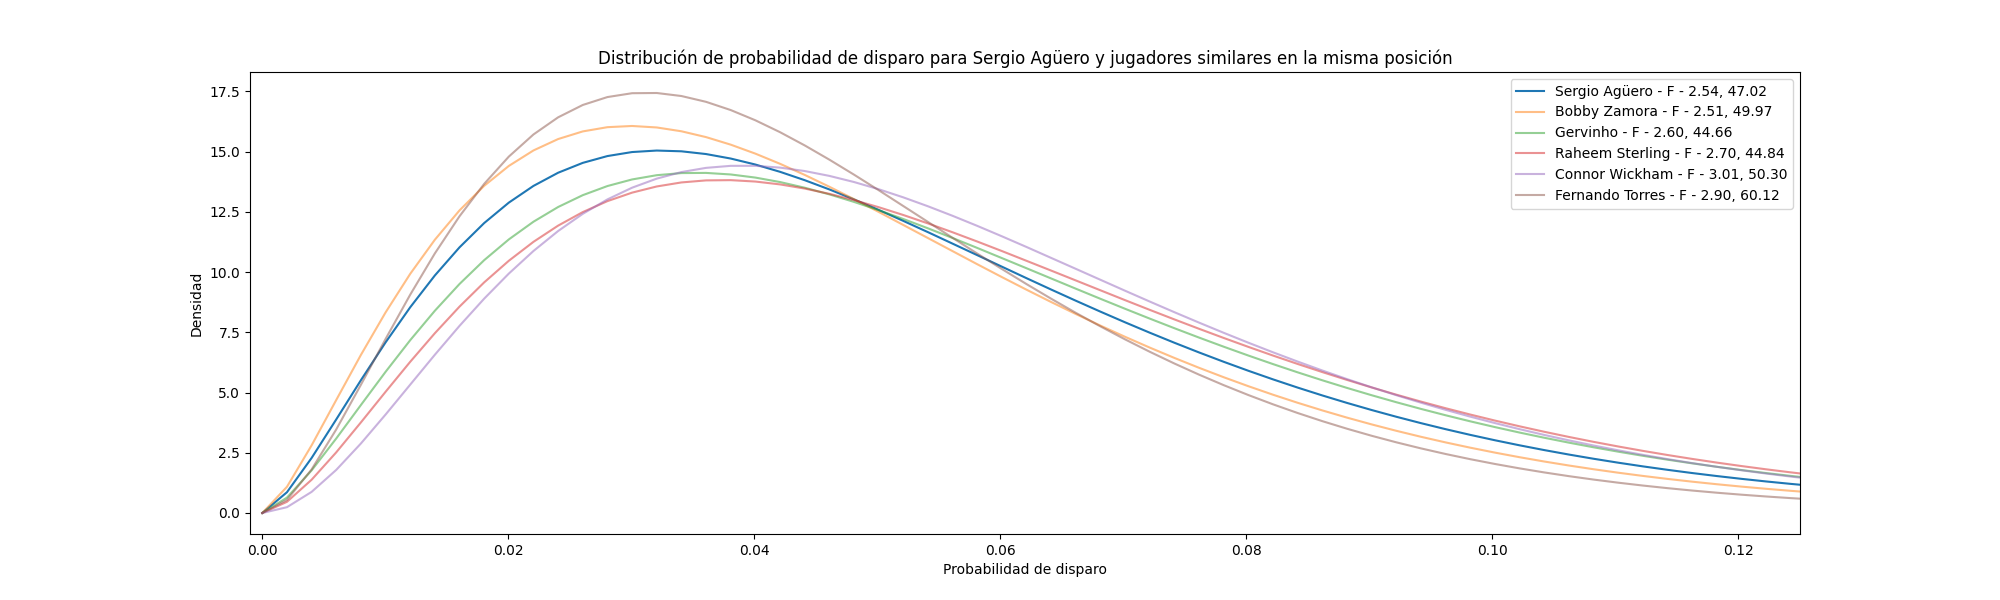
\includegraphics{recursos_pdf/graficos/Sergio_Aguero_and_similar_players_same_position_shots_prob_beta_binomial.png}
    \caption{Distribución de los $r(J, S)$ de jugadores similares a Sergio Agüero de la misma posición}
\end{figure}

Para conocer mejor la varianza de las distribuciones de los \(r(J, S)\)
de los jugadores, se estudió la distribución de los parámetros
\(\alpha\) y \(\beta\) de las distribuciones beta ajustadas. Hicimos un
análisis de clustering para agrupar a los jugadores en base a sus
distribuciones de los \(r(J, S)\).

\begin{figure}
  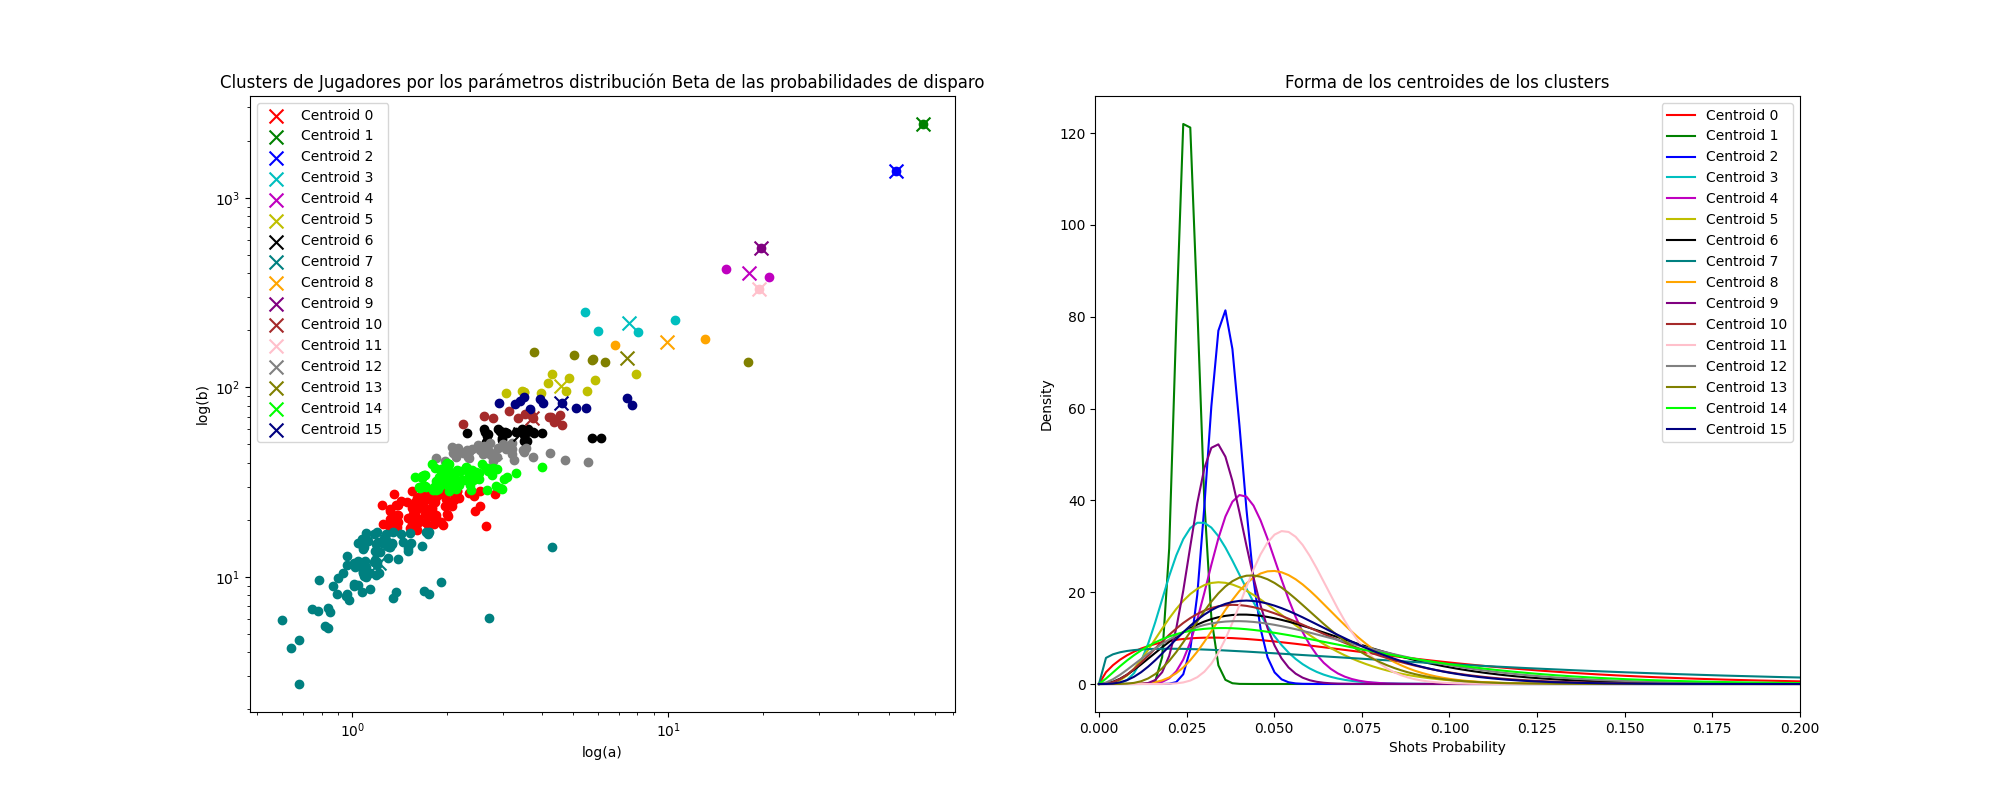
\includegraphics{recursos_pdf/graficos/Clusters_of_Players_shots_prob_beta_binomial.png}
    \caption{Distribución de los parámetros $\alpha$ y $\beta$ de los $r(J, S)$ de los jugadores}
\end{figure}

Como un extra, este sistema de clustering nos permite hallar rápido
jugadores similares entre sí. A partir de los clusters la siguiente
figura presenta las posibles distribuciones en cada cluster.

\begin{figure}
  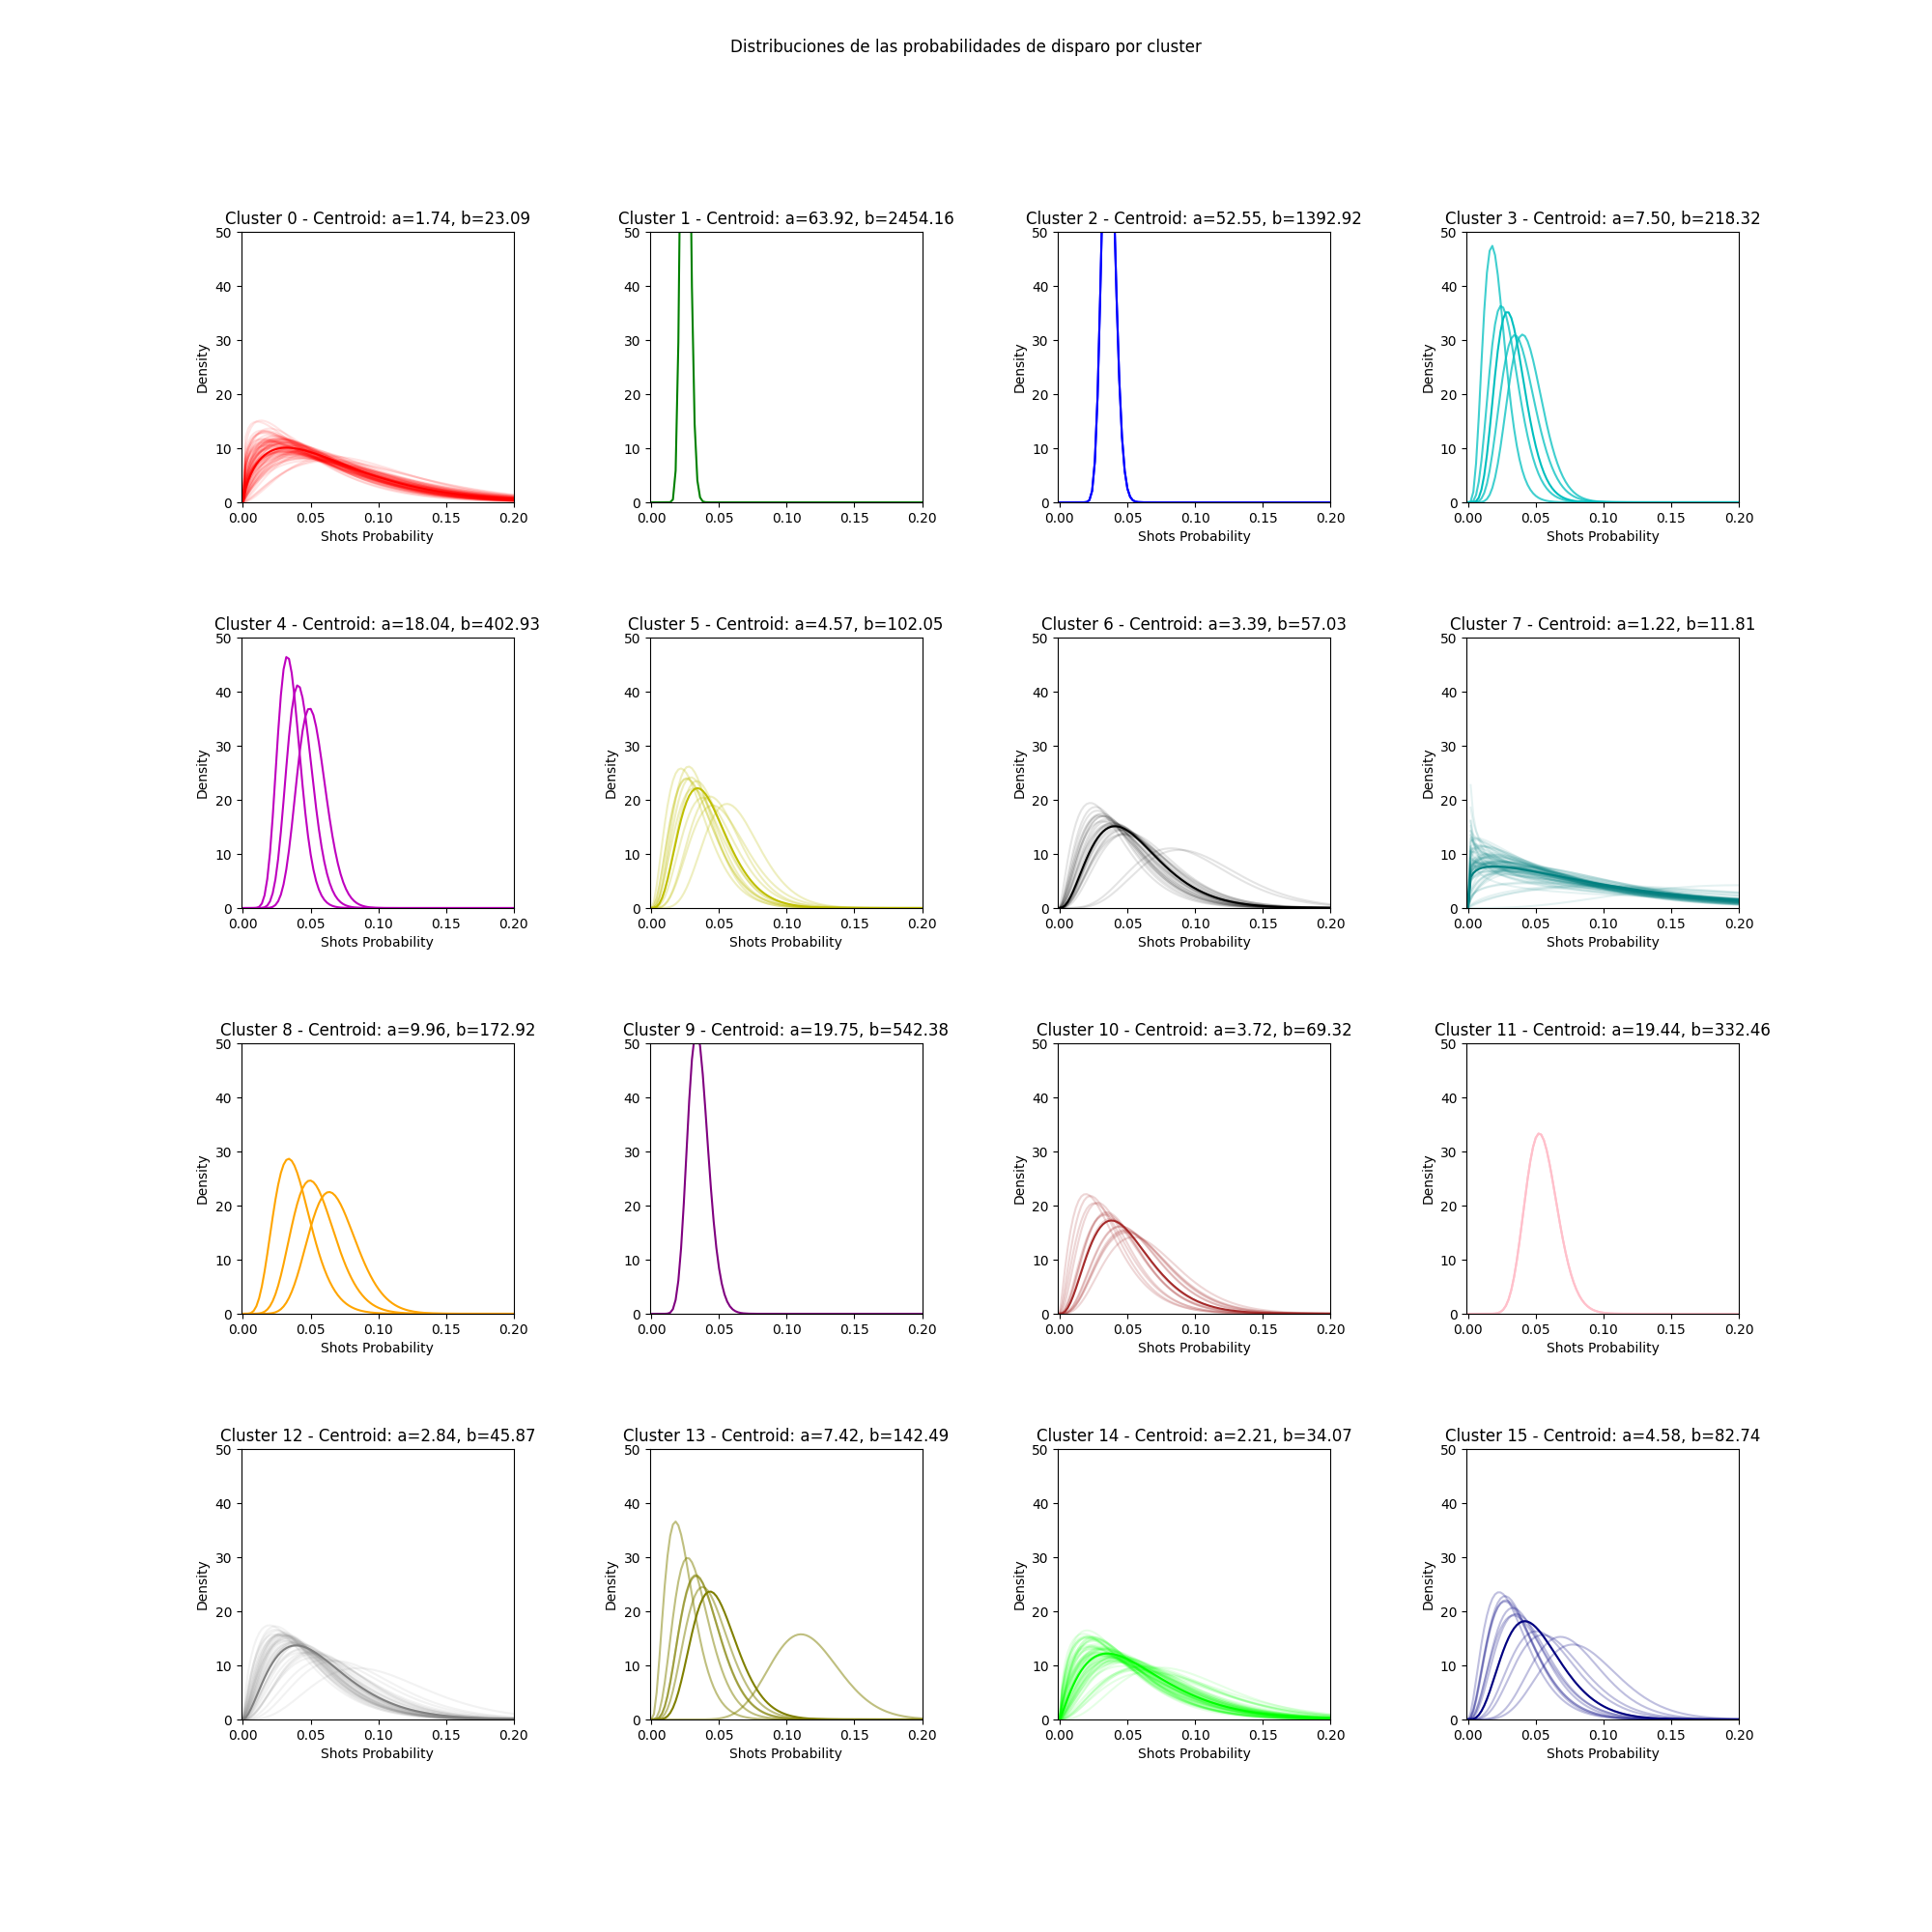
\includegraphics{recursos_pdf/graficos/Clusters_of_Players_shots_prob_beta_binomial_distributions.png}
    \caption{Distribución de los $r(J, S)$ de jugadores en clusters}
\end{figure}

\newpage

\hypertarget{estimaciuxf3n-de-la-distribuciuxf3n-del-psl}{%
\section{\texorpdfstring{\textbf{Estimación de la Distribución del
PSL}}{Estimación de la Distribución del PSL}}\label{estimaciuxf3n-de-la-distribuciuxf3n-del-psl}}

A partir de los resultados obtenidos en el análisis de las
distribuciones de los \(r(J, S)\), se propone un utilizar estas como
priors para cada jugador, es decir, se asume que la distribución de los
\(r(J, S)\) de un jugador es la distribución a priori de la variable
aleatoria \(r(J, S)\) para ese jugador, lo mismo para los
\(r(J_i, J_j)\), los \(r(J, L)\) y los \(r(J, G)\).

De esta forma, cada jugador \(J\) tiene una distribución a priori para
cada uno de los 14 estados, considerando esto, podemos reformular la
matriz de ratios de transición como una matriz de variables aleatorias
donde cada una se distribuye según la distribución a priori del jugador
correspondiente.

\hypertarget{variables-aleatorias-para-los-ru-v-y-psl-por-priors}{%
\subsection{\texorpdfstring{Variables Aleatorias para los \(r(U, V)\) y
PSL por
Priors}{Variables Aleatorias para los r(U, V) y PSL por Priors}}\label{variables-aleatorias-para-los-ru-v-y-psl-por-priors}}

Para actualizar la notación, sean \(r_{J, V}\) la variable aleatoria que
representa la ratio de transición entre el jugador \(J\) y el estado
\(V\), esto incluye \(r_{J, S}\), \(r_{J, L}\) y tambien \(r_{G, J}\),
asi como los \(r_{J_i, J_j}\) para \(i, j \in [1, 11]\).

Luego \(r_{J, V} \sim F_x\) la distribución a priori de la variable
aleatoria \(r_{J, V}\).

Para generalizar el analisis de distribuciones planteadas en la sección
anterior, se propone utilizar una distribución KDE (Kernel Density
Estimation) a partir de los histogramas de los \(r(J, V)\) para modelar
sus distribuciones, ya que no todos los ratios de transición siguen una
distribución beta tan bien como los \(r(J, S)\).

Finalmente obtenemos, para una formación dada de 11 jugadores, una
matriz de variables aleatorias \(\mathbf{R}\).

\[
    \mathbf{R} = \begin{pmatrix}
        0 & r_{G, J_1} & \dots & r_{G, J_{11}} & 0 & 0 \\
        0 & 0 & \dots & r_{J_1, J_{11}} & r_{J_1, L} & r_{J_1, S} \\
        \vdots & \vdots & \ddots & \vdots & \vdots & \vdots \\
        0 & r_{J_{11}, J_1} & \dots & 0 & r_{J_{11}, L} & r_{J_{11}, S} \\
        0 & 0 & \dots & 0 & 1 & 0 \\
        0 & 0 & \dots & 0 & 0 & 1 \\
    \end{pmatrix}
\]

Para mejor claridad, la siguiente vizualiación muestra la matriz de
variables aleatorias \(\mathbf{R}\) para un equipo de ejemplo. En cada
posición se observa la distribución a priori de la variable aleatoria
correspondiente.

\begin{figure}
  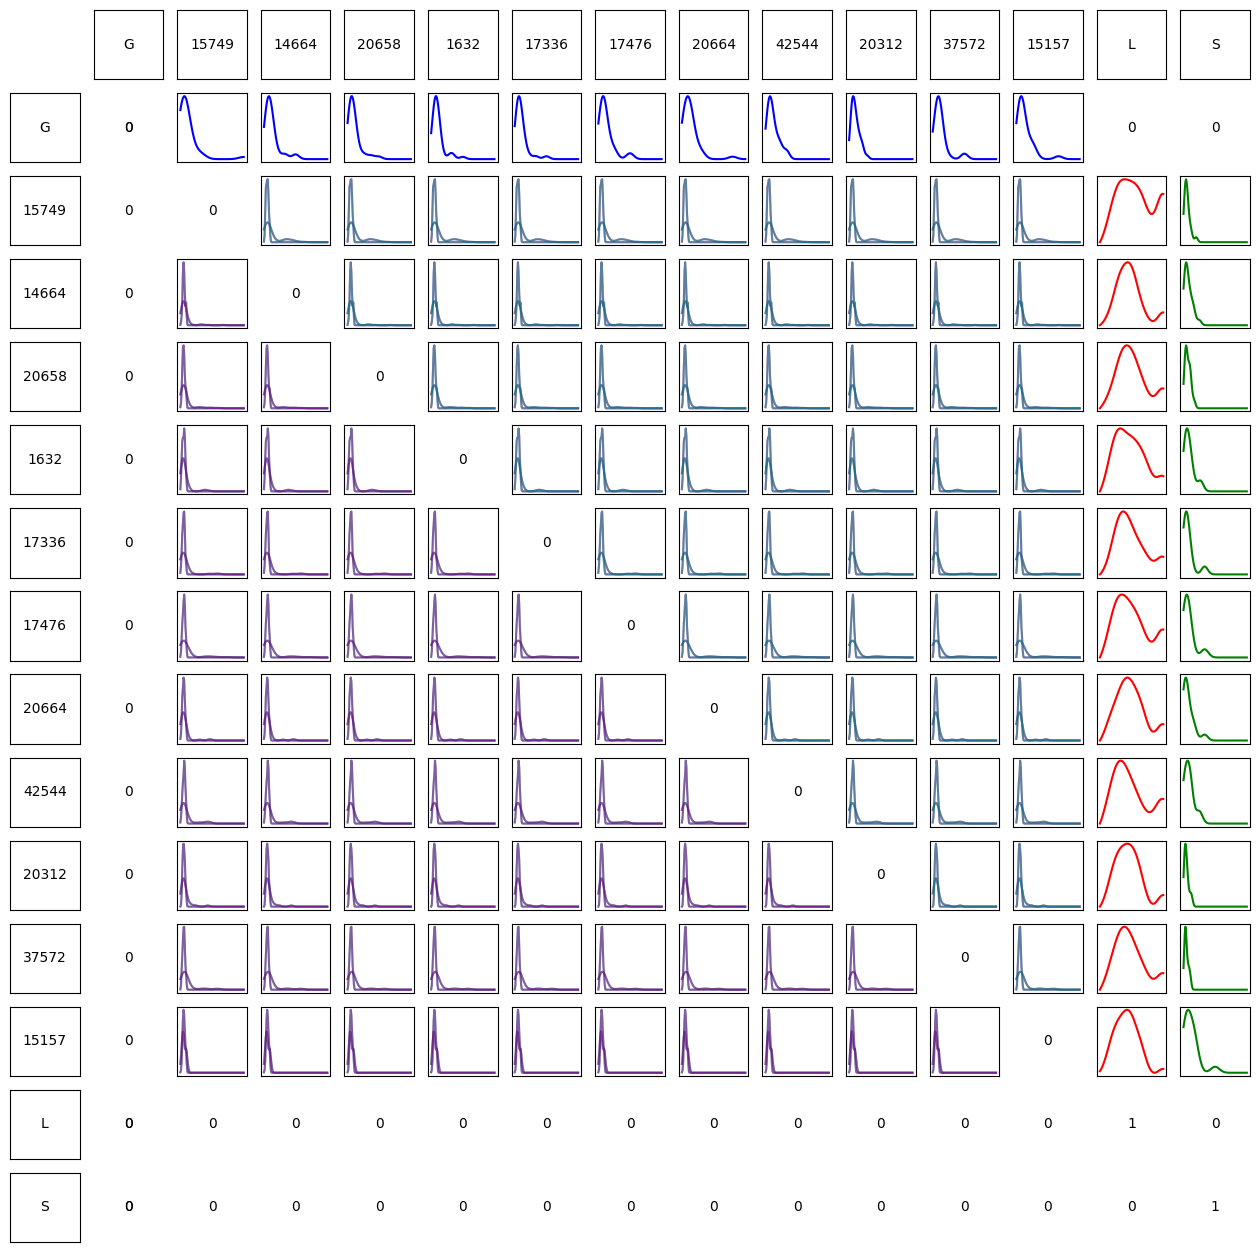
\includegraphics{recursos_pdf/graficos/f9090710-1703-476a-b906-8fddde8ae6d6.png}
    \caption{Matriz de Variables Aleatorias $\mathbf{R}$}
\end{figure}

\hypertarget{proceso-de-monte-carlo-para-estimar-la-distribuciuxf3n-del-psl}{%
\subsection{Proceso de Monte Carlo para estimar la distribución del
PSL}\label{proceso-de-monte-carlo-para-estimar-la-distribuciuxf3n-del-psl}}

Dado un equipo \(A\) con una formación de 11 jugadores \(L_A\), se busca
estimar la distribución del PSL de ese equipo a partir de las
distribuciones a prior de los \(r(U, V)\) de cada jugador. Para ello, se
propone un proceso de Monte Carlo para muestrear de las distribuciones a
priori de los \(r(U, V)\).

De la formación \(L_A\) podemos construir la matriz de variables
aleatorias \(\mathbf{R}\) a partir de las distribuciones a priori de los
\(r(U, V)\) de cada jugador.

Definimos \(\hat{f}^{N}_{PSL}(L_A)\) como la función distribución de
probabilidad empírica de los \(PSL_i\) para la formación \(L_A\) en base
a \(N\) simulaciones.

El proceso de Monte Carlo para estimar la distribución del PSL de la
formación \(L_A\) es el siguiente:

\begin{algorithm}[H]
\caption{Simulación del PSL del equipo $A$}\label{alg:cap}
\SetAlgoLined
\KwIn{Número de simulaciones $N$}
\KwIn{Formación $L_A$ = $\{J_1, J_2, \dots, J_{11}\}$}
\KwOut{Distribución del PSL del equipo $A$}
$\mathbf{R} \gets$ Construir la matriz de variables aleatorias a partir de las distribuciones a priori de los $r(U, V)$ de cada jugador\;
$PSL_i \gets 0$ para $i = 1, 2, \dots, N$\;
\For{$i = 1$ \KwTo $N$}{
    $R \gets $ Muestrear de la matriz $\mathbf{R}$ distribuciones a priori de los $r(U, V)$\;
    $Q \gets$ Normalizar las filas de $R$\;
    $PSL_i \gets PSL(Q)$\;
}
Estimar la distribución del PSL del equipo $A$ a partir de las $N$ observaciones obtenidas de las simulaciones\;
\end{algorithm}

A partir de esta distribución del PSL, se puede realizar comparaciones
entre diferentes formaciones de 11 jugadores.

El siguiente gráfico muestra la distribución del PSL de un equipo de
ejemplo obtenida a partir de 1000 simulaciones del proceso de Monte
Carlo para la formación mas utilizada en la temporada 2012/13 de la EPL
del equipo Manchester City.

\begin{figure}
  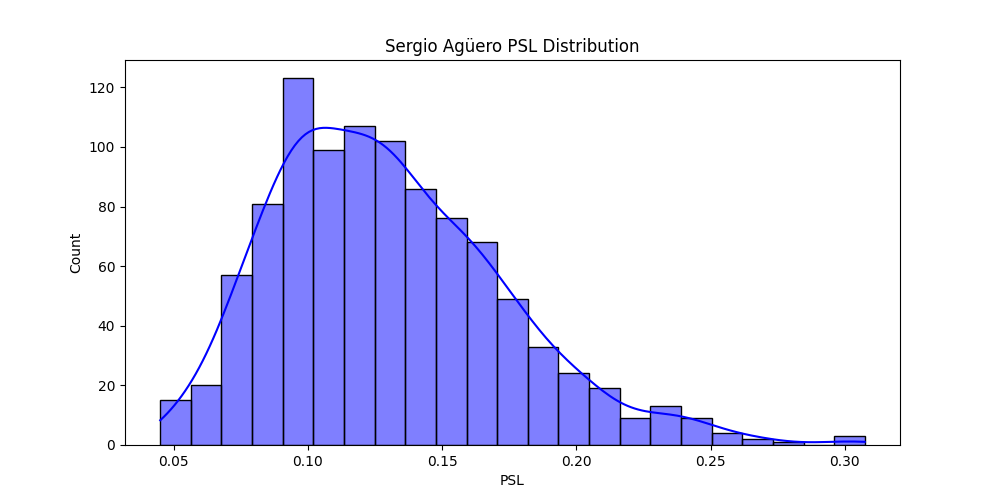
\includegraphics{recursos_pdf/graficos/sergio_aguero_psl_distribution.png}
    \caption{Distribución del PSL del equipo Manchester City}
\end{figure}

\hypertarget{comparar-el-impacto-sobre-el-psl-de-dos-jugadores-en-una-formaciuxf3n}{%
\subsection{Comparar el impacto sobre el PSL de dos jugadores en una
formación}\label{comparar-el-impacto-sobre-el-psl-de-dos-jugadores-en-una-formaciuxf3n}}

Para comparar el PSL de dos jugadores en una formación, se propone un
análisis de sensibilidad que consiste en evaluar el impacto en la
distribución del PSL al reemplazar a un jugador por otro en la
formación. El proceso para ello es el siguiente:

Se define la Formación \(L_A\) = \(\{J_1, J_2, \dots, J_{11}\) como la
formación original del equipo \(A\), donde alguno de los jugadores
\(J_i\) es el jugador a ``original''.

Se define el jugador \(J'\) a comparar con \(J_i\) y la formación
\(L'_A\) = \(\{J_1, J_2, \dots, J_{11}\}\) como la formación con el
jugador \(J'\) en lugar de \(J_i\).

Luego, se puede computar \(\hat{f}^{N}_{PSL}(L_A)\) y
\(\hat{f}^{N}_{PSL}(L'_A)\) para comparar las distribuciones del PSL de
las formaciones \(L_A\) y \(L'_A\).

\hypertarget{comparaciuxf3n-de-distribuciones-de-psl}{%
\subsection{Comparación de Distribuciones de
PSL}\label{comparaciuxf3n-de-distribuciones-de-psl}}

En la siguiente sección postulamos una serie de métodos y métricas para
comparar distribuciones de PSL de dos formaciones. En orden creciente de
complejidad y rigurosidad, proponemos:

\begin{enumerate}
\def\labelenumi{\arabic{enumi}.}
\tightlist
\item
  Comparación de Momentos Estadísticos
\item
  Dominancia Probabilística
\item
  Dominancia Estocástica
\end{enumerate}

Para explicar la comparación de distribuciones de PSL, se propone un
ejemplo de dos formaciones de 11 jugadores distintas, en una formación
\(L_{MC}\) se encuentran 10 jugadores del equipo Manchester City +
Sergio Agüero y en la otra \(L_{MC}^{\text{Giroud}}\) los mismos 10
jugadores + Olivier Giroud del equipo Arsenal.

Se realizó el proceso de Monte Carlo para estimar la distribución del
PSL de cada formación a partir de 1000 simulaciones. Luego en la figura
se puede observar las funciones de densidad de probabilidad aproximadas
de las distribuciones del PSL de las formaciones
\(\hat{f}^{1000}_{PSL}(L_{MC})\) y
\(\hat{f}^{1000}_{PSL}(L_{MC}^{\text{Giroud}})\).

\hypertarget{comparaciuxf3n-de-momentos-estaduxedsticos}{%
\subsubsection{Comparación de Momentos
Estadísticos}\label{comparaciuxf3n-de-momentos-estaduxedsticos}}

\begin{figure}
  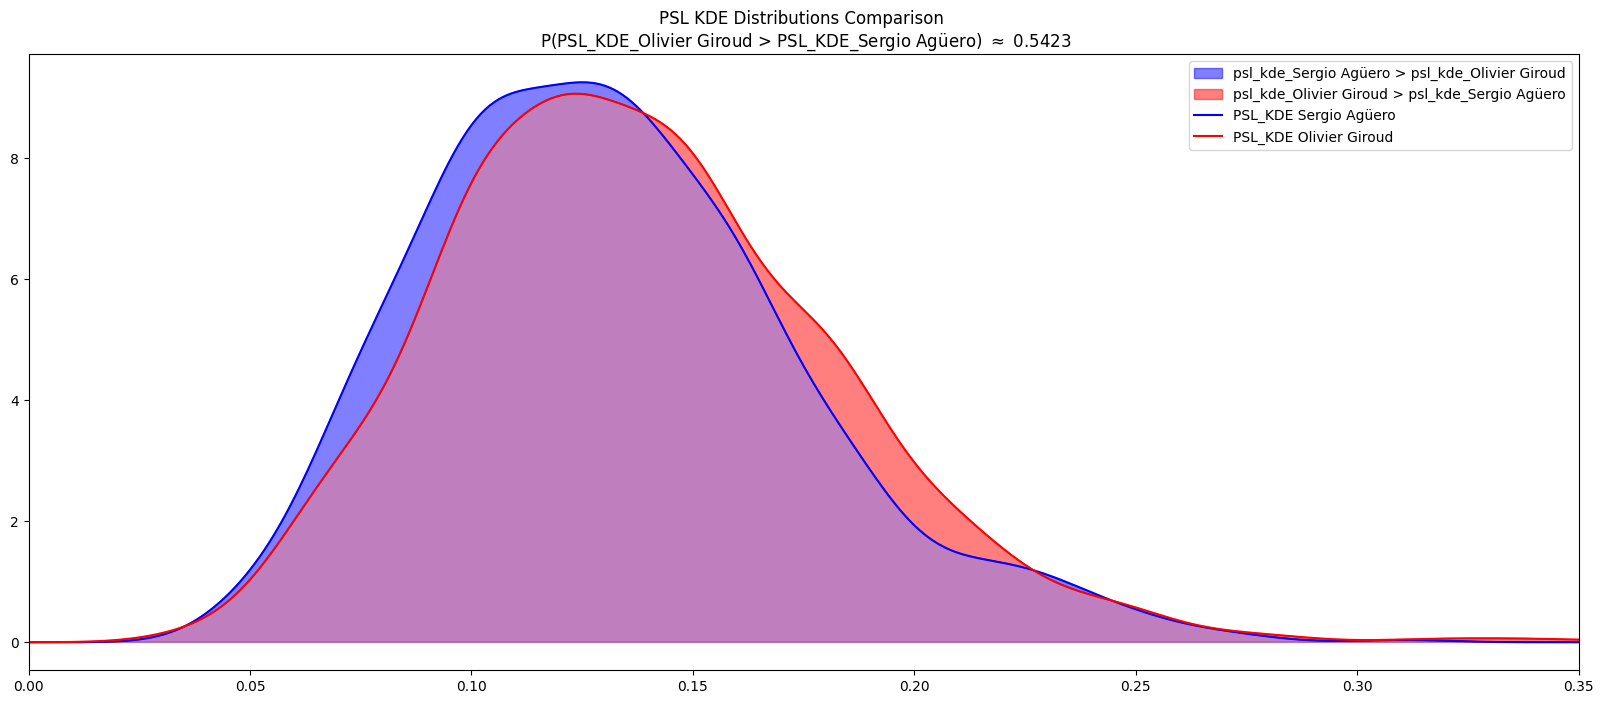
\includegraphics{./recursos_pdf/graficos/psl_dists_aguero_v_giroud.png}
    \caption{Ejemplo de dos distribuciones de PSL de dos formaciones distintas}
\end{figure}

Una posible comparación entre las distribuciones de PSL de dos
formaciones es ``a ojo'' observando las funciones de densidad de
probabilidad. En este caso puntual se puede observar como el equipo con
Agüero tiene una distribución de PSL mas sesgada a la izquierda que el
equipo con Giroud.

En un enfoque mas númerico, se puede realizar una comparación por
momentos de las distribuciones de PSL de dos formaciones. Se propone
comparar la media y la varianza de las distribuciones
\(\hat{f}^{1000}_{PSL}(L_{MC})\) y
\(\hat{f}^{1000}_{PSL}(L_{MC}^{\text{Giroud}})\) ya que el método de
Monte Carlo nos permite obtener una muestra significativa de las
distribuciones. Al no ser distribuciones normales, la skewness y la
kurtosis nos proveen información adicional sobre la forma de la
distribución.

\begin{table}
\caption{Comparación de momentos de $\hat{f}^{1000}_{PSL}(L_{MC})$ y $\hat{f}^{1000}_{PSL}(L_{MC}^{\text{Giroud}})$}
\label{tab:comparacion_momentos_psl}
\begin{center}
\begin{tabular}{llllll}
\toprule
Jugador & Media & Varianza & Desvio Estándar & Skewness & Kurtosis \\
\midrule
Aguero & 0.130861 & 0.041160 & 0.001694 & 0.554998 & 0.362611 \\
Giroud & 0.134403 & 0.043310 & 0.001876 & 0.580404 & 0.405658 \\
\bottomrule
\end{tabular}
\end{center}
\end{table}

Para este caso de ejemplo, se observa que la media y la varianza de las
distribuciones de PSL de la formación \(L_{MC}\) y
\(L_{MC}^{\text{Giroud}}\) son similares, aunque mayores en la formación
con Giroud. Además, el tercer momento (skewness) nos confirma lo
observado ``a ojo'' en las funciones de densidad de probabilidad, la
distribución de PSL de la formación con Agüero es mas sesgada a la
izquierda que la de la formación con Giroud. Por último el cuarto
momento (kurtosis) nos indíca que la
\(\hat{f}^{1000}_{PSL}(L_{MC}^{\text{Giroud}})\) tiene colas mas pesadas
que la \(\hat{f}^{1000}_{PSL}(L_{MC})\).

\hypertarget{dominancia-probabiluxedstica}{%
\subsubsection{Dominancia
Probabilística}\label{dominancia-probabiluxedstica}}

Otra forma de comparar las distribuciones de PSL de dos formaciones es a
través de la dominancia probabilística.

En este caso, se puede calcular la probabilidad de que una muestra
aleatoria de una distribución sea mayor que una muestra aleatoria de la
otra distribución. De esta forma podemos tomar samples de las
distribuciones \(\hat{f}^{1000}_{PSL}(L_{MC})\) y
\(\hat{f}^{1000}_{PSL}(L_{MC}^{\text{Giroud}})\) y calcular la
probabilidad de que un sample de la formación con Giroud sea mayor que
un sample de la formación con Agüero.

Sean \(X_{L_{MC}} \sim \hat{f}^{1000}_{PSL}(L_{MC})\) y
\(X_{L_{MC}^{\text{Giroud}}} \sim \hat{f}^{1000}_{PSL}(L_{MC}^{\text{Giroud}})\)
las variables aleatorias que se distribuyen según las distribuciones de
PSL de las formaciones \(L_{MC}\) y \(L_{MC}^{\text{Giroud}}\)
respectivamente. Luego para evaluar si la formación con Giroud tiene
dominancia probabilística sobre la formación con Agüero, se puede
calcular la probabilidad \(P(X_{L_{MC}^{\text{Giroud}}}>X_{L_{MC}})\).

El algoritmo para calcular la dominancia probabilística es el siguiente:

\begin{algorithm}[H]
\caption{Dominancia Probabilística}\label{alg:cap2}
\SetAlgoLined
\KwIn{Distribuciones de PSL $\hat{f}^{1000}_{PSL}(L)$ y $\hat{f}^{1000}_{PSL}(L')$}
\KwOut{Probabilidad de que un sample de PSL de la formación $L$ sea mayor que un sample de PSL de la formación con $L'$}
$N \gets 1000$\;
$M \gets 0$\;
\For{$i = 1$ \KwTo $N$}{
    $PSL \gets$ Muestrear de $\hat{f}^{1000}_{PSL}(L)$\;
    $PSL' \gets$ Muestrear de $\hat{f}^{1000}_{PSL}(L')$\;
    \If{$PSL' > PSL$}{
        $M \gets M + 1$\;
    }
}
$P \gets \frac{M}{N}$\;
\end{algorithm}

Para el caso de ejemplo, se obtuvo que la probabilidad de que un sample
de PSL de la formación con Giroud sea mayor que un sample de PSL de la
formación con Agüero es
\(P(X_{L_{MC}^{\text{Giroud}}}>X_{L_{MC}}) \approx 0.5423\). De esta
forma podemos concluir que la formación con Giroud tiene dominancia
probabilística sobre la formación con Agüero.

\hypertarget{comparaciuxf3n-de-cdfs-de-las-distribuciones-de-psl}{%
\subsubsection{Comparación de CDFs de las distribuciones de
PSL}\label{comparaciuxf3n-de-cdfs-de-las-distribuciones-de-psl}}

Otra forma de comparar las distribuciones de PSL de dos formaciones es a
través de las funciones de distribución acumulada (CDF). Llamemos
\(\hat{F}^{N}_{PSL}(L)\) a la función de distribución acumulada de PSL
obtenida a partir de \(N\) simulaciones del proceso de Monte Carlo para
la formación \(L\).

En la siguiente figura se observa la comparación de las CDFs de las
distribuciones de PSL de las formaciones \(L_{MC}\) y
\(L_{MC}^{\text{Giroud}}\).

\begin{figure}
  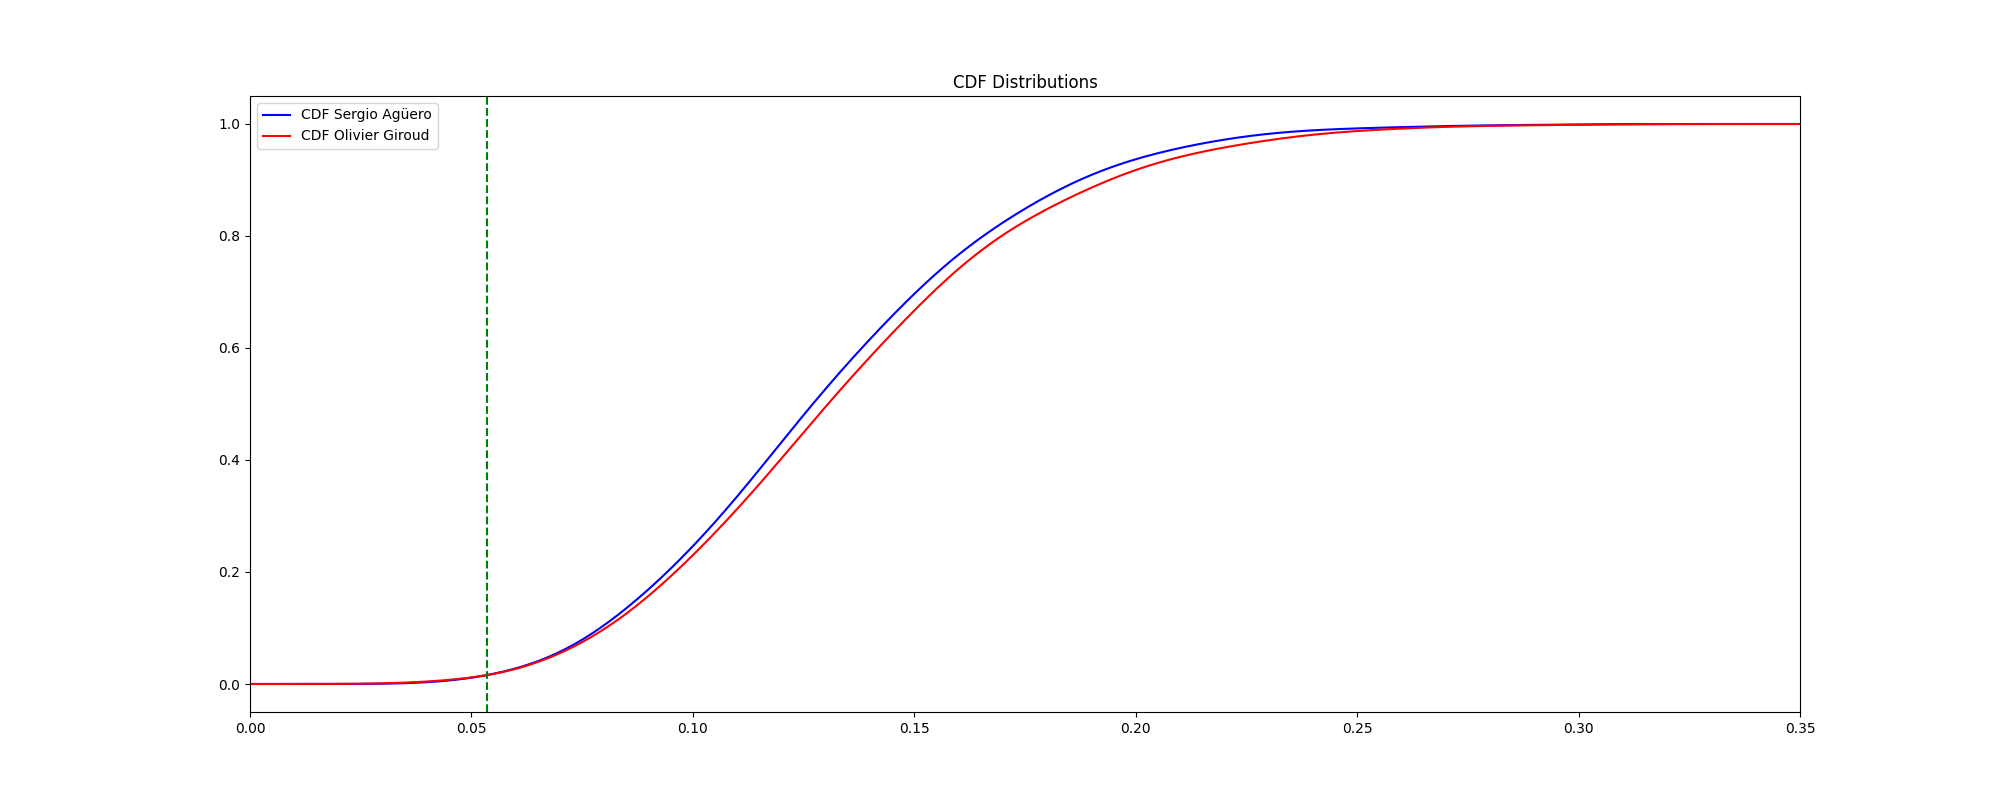
\includegraphics{./recursos_pdf/graficos/sergio_aguero_olivier_giroud_cdf_intersection.png}
    \caption{Comparación de CDFs de las distribuciones de PSL de las formaciones $L_{MC}$ y $L_{MC}^{\text{Giroud}}$}
\end{figure}

Nuevamente ``a ojo'' se puede analisar la relación entre las
distribuciones \(\hat{F}^{1000}_{PSL}(L_{MC})\) y
\(\hat{F}^{1000}_{PSL}(L_{MC}^{\text{Giroud}})\), en este caso podemos
ver como la CDF de la formación con Agüero es menor a la de la formación
con Giroud en la mayoría de los puntos, lo que indica que la formación
con Agüero tiene un PSL menor que la formación con Giroud en la mayoría
de los casos.

\hypertarget{dominancia-estocuxe1stica}{%
\subsubsection{Dominancia Estocástica}\label{dominancia-estocuxe1stica}}

Mas formalmente se puede evaluar la dominancia estocástica entre las
CDFs \(\hat{F}^{1000}_{PSL}(L_{MC})\) y
\(\hat{F}^{1000}_{PSL}(L_{MC}^{\text{Giroud}})\). La dominancia
estocástica es una relación de orden entre dos funciones de distribución
acumulada que indica si una distribución es mayor que la otra en todos
los puntos.

Especificamente, podemos ver que apartir del umbral resaltado en verde
en la figura (\(x = 0.05346757\)),
\(\hat{F}^{1000}_{PSL}(L_{MC}^{\text{Giroud}})\) tiene
\textbf{dominancia estocástica} \emph{parcial} sobre
\(\hat{F}^{1000}_{PSL}(L_{MC})\) (Bawa, 1982; Gustavo, n.d.-a).

\hypertarget{conclusiones-sobre-la-comparaciuxf3n-de-distribuciones-de-psl}{%
\subsubsection{Conclusiones sobre la Comparación de Distribuciones de
PSL}\label{conclusiones-sobre-la-comparaciuxf3n-de-distribuciones-de-psl}}

Dependiendo el grado de rigurosidad provista por una comparación previa,
recomendamos contemplar algúno de los consecuentes métodos presentados
para comparar distribuciones de PSL. En este caso de ejemplo, se observó
que la formación con Giroud tiene dominancia probabilística sobre la
formación con Agüero aunque no se puede afirmar que tiene dominancia
estocástica.

La comparación por momentos es una forma rápida y sencilla de comparar
distribuciones de PSL, sin embargo, no siempre refleja la relación entre
las distribuciones. La dominancia probabilística es una métrica
intuitiva que nos permite evaluar la probabilidad de que una muestra de
una distribución sea mayor que una muestra de la otra distribución. Por
último, la dominancia estocástica es una relación de orden más rigurosa
que nos permite evaluar si una distribución es mayor que la otra en
todos los puntos.

El campo de estudio sobre la Dominancia Estocástica es amplio y
complejo, en esta investigación se presentó una humilde introducción al
tema y se propuso un método para evaluar la dominancia, por lo que se
recomienda profundizar en el tema para una mejor comprensión a la hora
de tomar desiciones basado en comparación de CDFs. Recomendamos la
publicación ``Stochastic Dominance: A Research Bibliography'' (Bawa,
1982) que contiene al rededor de 400 referencias sobre el tema.

\newpage

\hypertarget{player2vec-embeddings-de-jugadores}{%
\section{\texorpdfstring{\textbf{Player2Vec}: Embeddings de
Jugadores}{Player2Vec: Embeddings de Jugadores}}\label{player2vec-embeddings-de-jugadores}}

Para poder representar a cada jugador de forma vectorial, se desarrolló
el modelo de Player2Vec que permite obtener un embedding de cada jugador
en un espacio de \(n\) dimensiones.

Un embedding es una representación numérica de objetos en un espacio de
\(n\) dimensiones, donde propiedades o relaciones similares se
preservan. En el contexto de jugadores, un embedding transforma las
características de cada jugador en un vector de números, de tal manera
que jugadores con comportamientos o atributos similares estén más cerca
en este espacio vectorial. Esto facilita que modelos como redes
neuronales aprendan patrones complejos a partir de estas
representaciones compactas.

\hypertarget{definiciuxf3n}{%
\subsection{Definición}\label{definiciuxf3n}}

Player2Vec es una adaptación de Node2Vec para representar jugadores de
fútbol en un espacio vectorial. En este caso, los nodos del grafo
representan jugadores, y las aristas entre ellos reflejan la interacción
entre los jugadores en partidos de fútbol. A partir de los datos de
eventos de partidos (pases, disparos, goles, etc.), se construye un
grafo donde los nodos son jugadores y las aristas representan la
frecuencia de interacción entre ellos.

\hypertarget{modelado-de-la-epl-201213-como-grafo}{%
\subsection{Modelado de la EPL 2012/13 como
Grafo}\label{modelado-de-la-epl-201213-como-grafo}}

A partir de una formación de 11 (Lineup), para un equipo (Team), en un
partido (Match), se construye el grafo de la red de jugadores. Llamemos
a estos \(G_{L, T, M}\) Grafo de Lineup.

Sean:

\begin{itemize}
\tightlist
\item
  \(l \in L = \{0, 3\}\) las formaciones posibles (en la temporada 12/13
  se permitían hasta 3 cambios de jugadores)
\item
  \(t \in T = \{\text{Local}, \text{Visitante}\}\) los equipos que
  jugaron el partido.
\item
  \(m \in M = \{1, 2, \dots, 380\}\) los partidos de la temporada 12/13
  de la EPL
\end{itemize}

\[
\begin{aligned}
    G_{L, T, M} &= (V^{L, T, M}, E^{L, T, M}) \\
    L &= \text{Número de Lineup del equipo en el partido} \\
    T &= \text{Número de Equipo} \\
    M &= \text{Número de Partido} \\
    V^{L, T, M} &= \{\text{Gain}^{L, T, M}, J_1^{L, T, M}, J_2^{L, T, M}, \dots, J_{11}^{L, T, M}, \text{Loss}^{L, T, M}, 
    \text{Shot}^{L, T, M}\} \\
    E^{L, T, M} &= \{(J_i^{L, T, M}, J_j^{L, T, M}, r(J_i^{L, T, M}, J_j^{L, T, M})) \mid i, j \in [1, 11]\} \\ 
    & \cup \{(\text{Gain}^{L, T, M}, J_i^{L, T, M}, r(\text{Gain}^{L, T, M}, J_i^{L, T, M})) \mid i \in [1, 11]\} \\ 
    & \cup \{(J_i^{L, T, M}, \text{Shot}^{L, T, M}, r(J_i^{L, T, M}, \text{Shot}^{L, T, M})) \mid i \in [1, 11]\} \\ 
    & \cup \{(J_i^{L, T, M}, \text{Loss}^{L, T, M}, r(J_i^{L, T, M}, \text{Loss}^{L, T, M})) \mid i \in [1, 11]\}
\end{aligned}
\]

Donde cada \(J_i^{L, T, M} \mid i \in [1, 11]\) es un nodo que
representa a un jugador en el lineup \(L\) del equipo \(T\) en el
partido \(M\). \(Gain^{L, T, M}\) es el nodo que representa la ganancia
del balón, \(Loss^{L, T, M}\) la pérdida del balón y \(Shot^{L, T, M}\)
el disparo al arco en el lineup \(L\) del equipo \(T\) en el partido
\(M\).

En la figura se visualiza un ejemplo de un grafo de lineup
\(G^{L, T, M}\) genérico con los ejes \(r(J_1^{L, T, M}, U)\)
resaltados.

\begin{figure}
  
\includegraphics{recursos_pdf/graficos/G_LTM.png}
    \caption{Grafo de Lineup}
\end{figure}

Luego sean: - \(J_i \mid i \in [0, 522]\) los jugadores reales de la
temporada 2012/13 de la EPL

Se construye el grafo de la red de jugadores \(G_{\text{EPL-12/13}}\)
como la unión de todos los grafos de lineup \(G^{L, T, M}\).

\[
\begin{aligned}
   G_{\text{Full}} &= (V, E) = \bigcup_{L, T, M} G^{L, T, M} \\
   V &= \{J_1, J_2, \dots, J_{522}, Gain, Loss, Shot\} \\
    & \cup 
    \bigcup_{L, T, M} \{J_1^{L, T, M}, J_2^{L, T, M}, \dots, J_{11}^{L, T, M}, G^{L, T, M}, L^{L, T, M}, S^{L, T, M}\} \\
   E &= \bigcup_{L, T, M} E^{L, T, M} \\
   & \cup \{(J_i, J_j^{L, T, M}, r(J_i, J_j^{L, T, M})) \mid i \in [0, 522], j \in [1, 11], L, T, M\} \\
    & \cup \{(Gain, Gain^{L, T, M}, 1) \mid L, T, M\} \\
    & \cup \{(Loss^{L, T, M}, Loss, 1) \mid L, T, M\} \\
    & \cup \{(Shot^{L, T, M}, Shot, 1) \mid L, T, M\}
\end{aligned}
\]

El ratio de transición \(r(J_i, J_i^{L, T, M})\) es el tiempo jugado por
el Jugador \(J_i\) en el lineup \(L\) del equipo \(T\) en el partido
\(M\) sobre el tiempo total jugado por el Jugador \(J_i\)

\[
    r(J_i, J_i^{L, T, M}) = \frac{\text{Time Played}_{J_i^{L, T, M}}}{\text{Time Played}_{J_i}}
\]

La siguiente figura es una visualización de una instancia de un Equipo
en un Partido con sus lineups. En este caso el equipo hizo dos cambios
en el partido (\(J_4\) por \(J_{12}\) y \(J_2\) por \(J_{13}\)). Se
puede observar como los jugador reales \(J_4\) y \(J_{12}\) se
encuentran representados por el mismo nodo \(J_4^{L, T, M}\) y lo mismo
para \(J_2\) y \(J_{13}\) con \(J_2^{L, T, M}\) para sus respectivos
lineups. El resto de los nodos de jugadores reales mantienen su
identidad en los grafos de lineups.

\begin{figure}
  
\includegraphics{recursos_pdf/graficos/G_TM.png}
    \caption{Grafo de Jugadores}
\end{figure}

El grafo resultante de la composición de todos los grafos de lineup
\(G_{\text{Full}}\) se puede comprender mejor en la siguiente
visualización:

\begin{figure}
  \includegraphics{recursos_pdf/graficos/G_EPL_12_13.png}
    \caption{Grafo de Jugadores Completo}
\end{figure}

Donde al igual que en la figura anterior, los nodos de jugadores reales
se encuentran representados por los nodos de los lineups en los que
participaron.

El algoritmo en concreto para construir el grafo de la red de jugadores
\(G_{\text{Full}}\) es el siguiente:

\begin{algorithm}[H]
\caption{Construcción del Grafo de Jugadores}\label{alg:cap3}
\SetAlgoLined
\KwIn{Datos de eventos de partidos de la temporada 2012/13 de la EPL}
\KwOut{Grafo de la red de jugadores $G_{\text{Full}}$}
$V \gets \{J_1, J_2, \dots, J_{522}, Gain, Loss, Shot\}$\;
$E \gets \emptyset$\;
\For{partido $M$}{
    \For{lineup $L$ del partido $M$}{
        \For{jugador $J_i$ en el lineup $L$}{
            $V \gets V \cup \{J_i^{L, T, M}\}$\;
            $E \gets E \cup \{(J_i, J_i^{L, T, M}, r(J_i, J_i^{L, T, M}))\}$\;
        }
        $V \gets V \cup \{Gain^{L, T, M}, Loss^{L, T, M}, Shot^{L, T, M}\}$\;
        $E \gets E \cup \{(Gain, Gain^{L, T, M}, 1), (Loss^{L, T, M}, Loss, 1), (Shot^{L, T, M}, Shot, 1)\}$\;
    }
}
\end{algorithm}

\hypertarget{implementaciuxf3n}{%
\subsection{Implementación}\label{implementaciuxf3n}}

A partir de calcular las matrices de ratios \(R^{L, T, M}\) para cada
lineup \(L\) del equipo \(T\) en el partido \(M\) generamos el grafo
dirigido \(G^{L, T, M}\) haciendo uso de la librería \texttt{NetworkX}
en Python para luego componerlos en \(G_{\text{Full}}\), el grafo
resultante contiene 37521 nodos y 47338 aristas.

Para obtener los embeddings de los jugadores, se utilizó la librería
\texttt{node2vec} en Python, que implementa el algoritmo homónimo. Se
configuró el modelo con una longitud de caminata de 16 nodos, 200
caminatas y un tamaño de ventana de 12 nodos. Se entrenaron 2 modelos de
embeddings, uno con 64 dimensiones para utilizar en modelos de Deep
Learning y otro con 3 dimensiones.

Para cada uno de los 37521 nodos se obtuvo un embedding, de los cuales
nos quedamos solo con los 522 embeddings de los jugadores reales, estos
finalmente son la representación vectorial de cada jugador en el espacio
de embeddings.

Este modelo hace uso de Node2Vec, que es en sí una adaptación de
Word2Vec, una técnica de NLP que permite representar palabras en un
espacio vectorial (Grover \& Leskovec, 2016; Mikolov et al., 2013).

Node2Vec es un algoritmo que aprende representaciones vectoriales
(embeddings) para nodos en un grafo, preservando tanto las relaciones
locales como las globales entre ellos. Utiliza técnicas de random walks
para capturar el contexto de cada nodo, balanceando entre explorar nodos
cercanos y lejanos. Estos embeddings son útiles para tareas de machine
learning sobre grafos, ya que capturan de forma eficiente las
interacciones entre nodos en el grafo.

En el caso de Player2Vec, los \(k\) random walks resultantes son una
secuencia de jugadores y/o estados de juego en un partido de fútbol
(Ganancia, Pérdida, Disparo). A modo ilustrativo los siguientes son
posibles random walks obtenidos del grafo de la EPL 2012/13:

\[
\begin{aligned}
    & \text{Random Walk 1:} \text{ Gain} \rightarrow \text{Gain}^{L, T, M} \rightarrow J_1^{L, T, M} \rightarrow J_7^{L, T, M} \rightarrow \dots \rightarrow \text{Shot}^{L, T, M} \rightarrow \text{Shot} \\
    & \text{Random Walk 2:} \text{ } J_{93} \rightarrow J_{93}^{L, T, M} \rightarrow J_{15}^{L, T, M} \rightarrow J_{21}^{L, T, M} \rightarrow \text{Loss}^{L, T, M} \rightarrow \text{Loss} \\
    \vdots \\
    & \text{Random Walk} \text{ } k: \text{ } J_{12} \rightarrow J_{12}^{L, T, M} \rightarrow J_{13}^{L, T, M} \rightarrow J_{33}^{L, T, M} \rightarrow \text{Shot}^{L, T, M} \rightarrow \text{Shot} \\
\end{aligned}
\]

La cantidad de random walks \(k\) asi como los otros hiperparametros del
modelo de Node2Vec fueron seleccionados de forma empírica observando el
resultado de los embeddings obtenidos.

\hypertarget{visualizaciuxf3n-y-exploraciuxf3n-de-los-embeddings}{%
\subsection{Visualización y Exploración de los
Embeddings}\label{visualizaciuxf3n-y-exploraciuxf3n-de-los-embeddings}}

Para comenzar a explorar el espacio vectoriál generado por Player2Vec,
se ajustó un modelo inicialmente a partir siguientes hiperparametros:

\begin{itemize}
\tightlist
\item
  Dimensión de embeddings: 3
\item
  Longitud de caminata: 16 nodos
\item
  Número de caminatas: 200
\item
  Tamaño de ventana: 12 nodos
\end{itemize}

Se entrenó el modelo y se obtuvieron los embeddings de los 522 jugadores
de la temporada 2012/13 de la EPL. La siguiente visualización muestra
los embeddings de los jugadores en un espacio de 3 dimensiones, el color
corresponde al equipo en el que juega el jugador.

\begin{figure}
  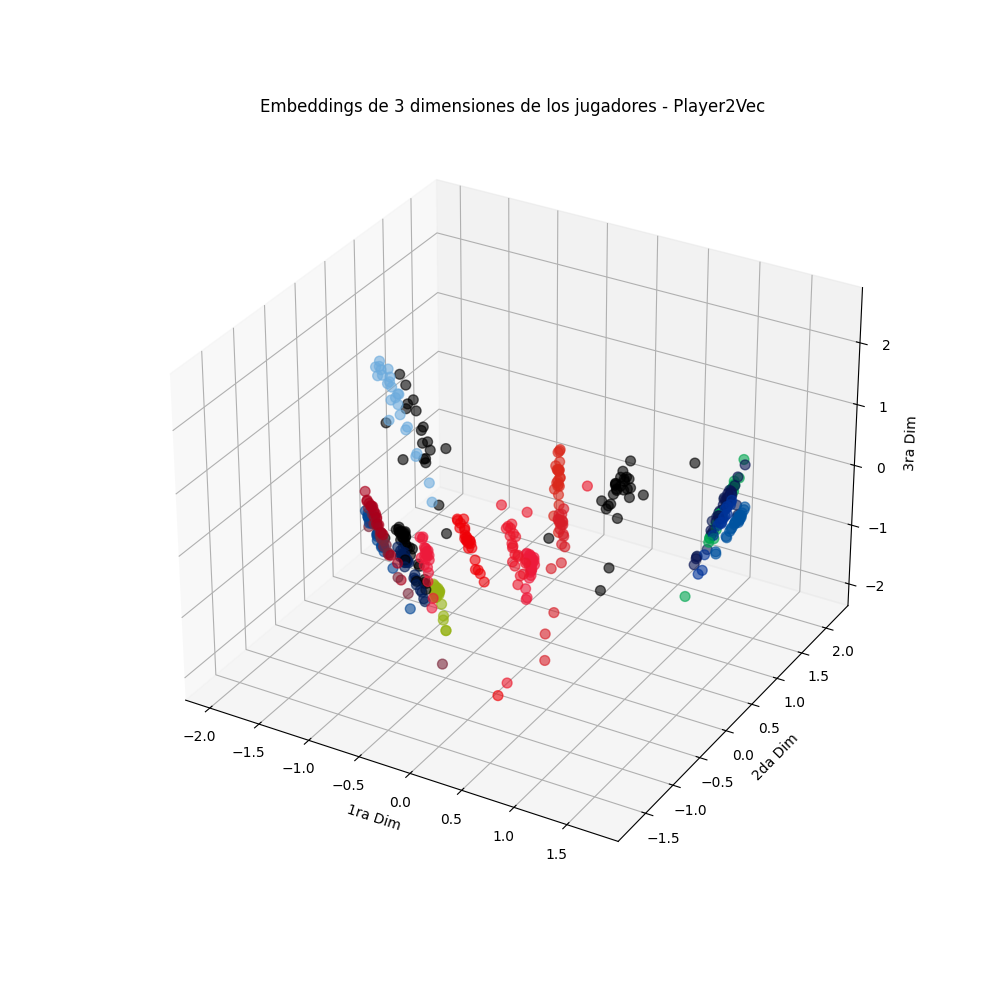
\includegraphics{recursos_pdf/graficos/players_3d.png}
    \caption{Embeddings de Jugadores en 3D}
\end{figure}

Para poder visualizar de forma más clara los embeddings de los
jugadores, se realizó un PCA para reducir la dimensionalidad de los
embeddings a 2 dimensiones. La siguiente visualización muestra los
embeddings de los jugadores en un espacio de 2 dimensiones, el color
corresponde al equipo en el que juega el jugador.

\begin{figure}
  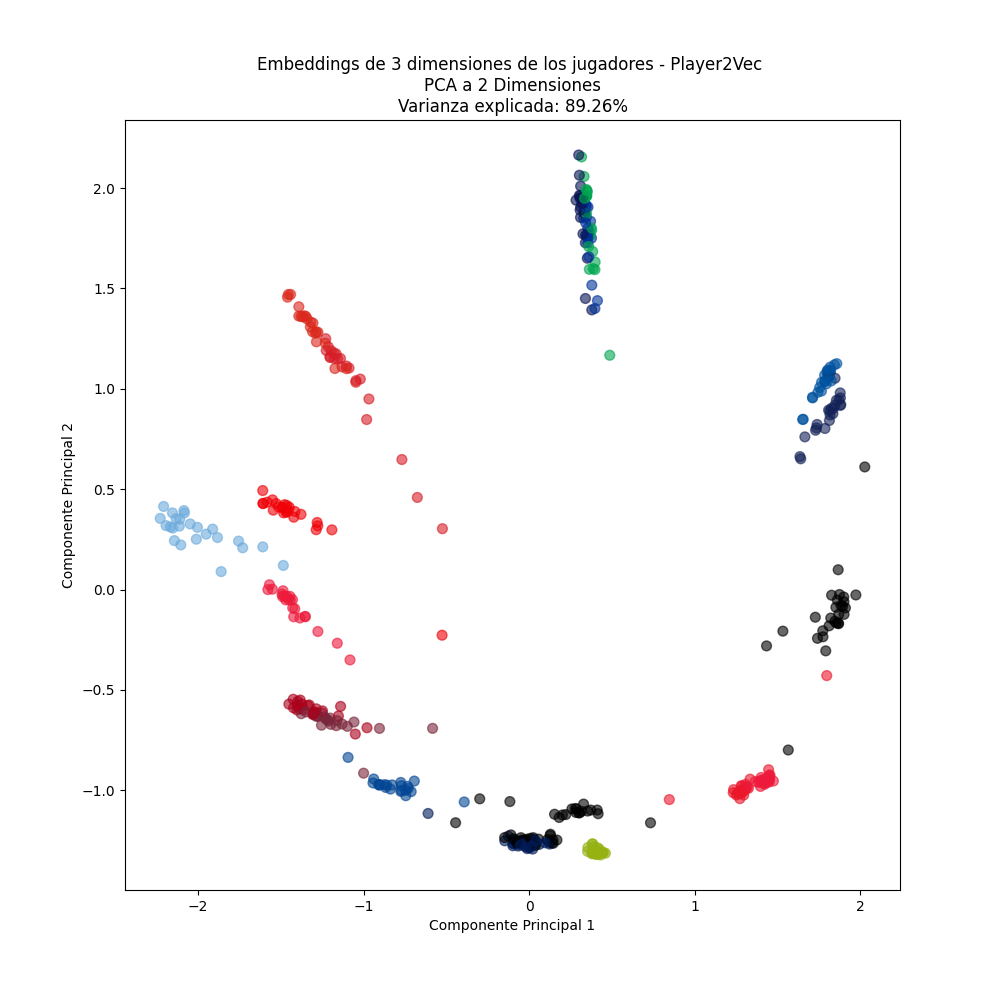
\includegraphics{recursos_pdf/graficos/players_3d_2d.png}
    \caption{Embeddings de Jugadores en 3D - PCA a 2D}
\end{figure}

En la figura de los componentes principales se observa como los
jugadores de un mismo equipo se encuentran cercanos en el espacio
vectorial, lo que indica que los embeddings resultantes de este modelo
capturan las relaciones entre los jugadores de un mismo equipo.

Ademas se observa como en este espacio las direcciones en las que se
representan a los equipos divergen de forma clara, lo que indica que los
embeddings capturan unicamente las diferencias entre los equipos y no
las similitudes. Buscan cierta ortogonalidad entre los equipos que no
logra existir en este espacio de 3 dimensiones.

Para explotar aún mas las relaciones a aprender por el modelo, se ajustó
un segundo modelo con las siguientes características:

\begin{itemize}
\tightlist
\item
  Dimensión de embeddings: 64
\item
  Longitud de caminata: 40 nodos
\item
  Número de caminatas: 500
\item
  Tamaño de ventana: 30 nodos
\end{itemize}

Luego para explorar los embeddings resultantes se realizó nuevamente un
analisis de componentes principales para reducir la dimensionalidad de
los embeddings a 2 dimensiones.

\begin{figure}
  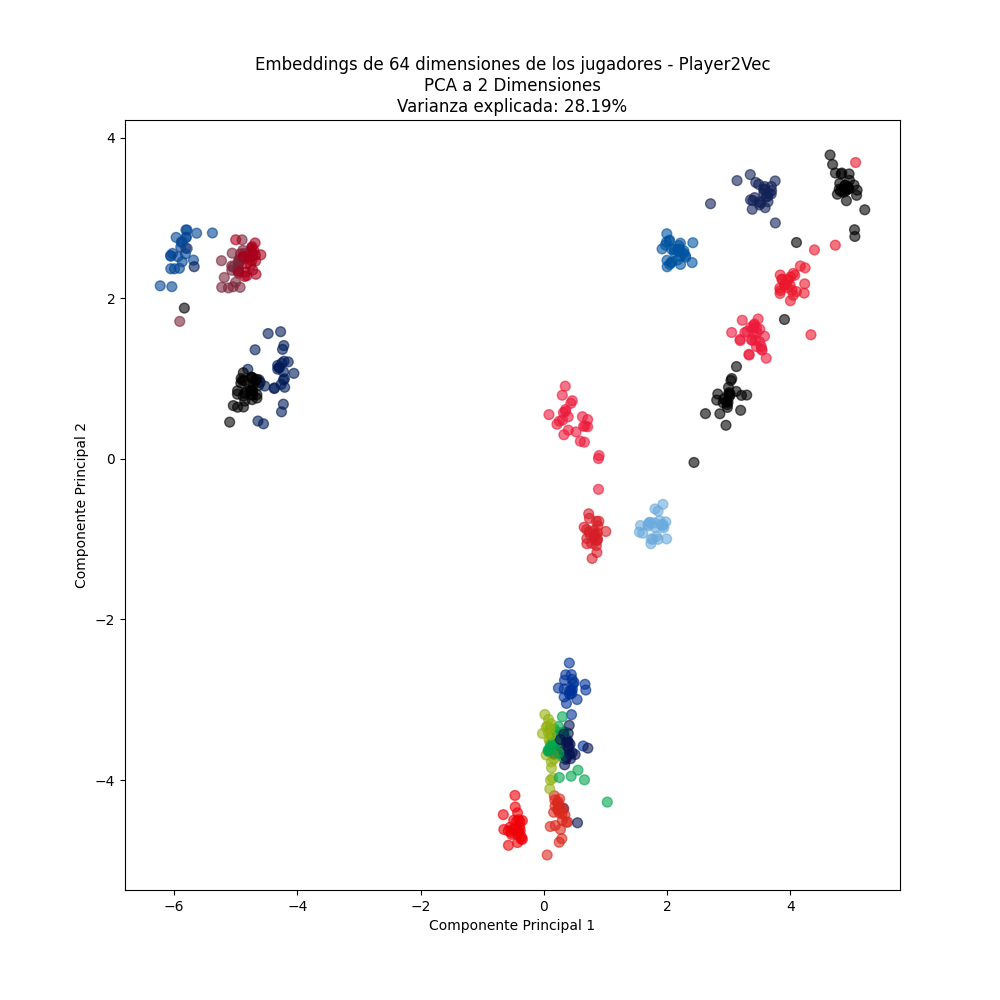
\includegraphics{recursos_pdf/graficos/players_64_2d.png}
    \caption{Embeddings de Jugadores en 64D - PCA a 2D}
\end{figure}

En esta figura resultante se puede observar como la direccionalidad de
los equipos desaparece pero se mantienen las relaciones entre los
jugadores de un mismo equipo.

\hypertarget{potencial-de-player2vec}{%
\subsection{Potencial de Player2Vec}\label{potencial-de-player2vec}}

Con el modelo planteado de Grafos de Lineups por Equipos y Partidos se
puede representar no solo una temporada de una liga, como es nuestro
caso, sino que se puede extender a múltiples temporadas y ligas. Esto
permitiría poder comparar jugadores de distintas ligas y temporadas, y
poder evaluar el rendimiento de un jugador en distintos contextos.

Otra cuestión considerada para expandir es ademas de tener un nodo
general por jugador conectado a sus instancias en cada lineup, se podría
tener un nodo que represente a un jugador en un equipo, de forma tal que
el jugador real esta conectado a su nodo ``Jugador en Equipo'' y este
nodo a su vez conectado a ``Jugador en Lineup de Partido de Equipo''.
Esto permitiría poder evaluar el rendimiento de un jugador en un equipo
en particular y como este se comporta en distintos contextos.

En el paper de \emph{Soccer Networks} donde se plantea el PSL definen
una serie de coeficientes \(h\), \(a\), \(\omega\), como la performance
de un equipo al jugar de local, al jugar de visitante, y la performance
ponderada de todos los otros equipos al jugar de visitante
respectivamente. Se podrían escalar los ratios de transición entre
jugadores y el estado de disparo al arco en función de estos
coeficientes para obtener una mejor representación de la performance de
un jugador en un partido en particular.

\newpage

\hypertarget{modelo-predictivo}{%
\section{\texorpdfstring{\textbf{Modelo predictivo de Distribuciones de
Ratios de Transición}
(\(r(U, V)\))}{Modelo predictivo de Distribuciones de Ratios de Transición (r(U, V))}}\label{modelo-predictivo}}

El trabajo de Player2Vec nos permite obtener embeddings de jugadores que
capturan las relaciones entre ellos en un espacio vectorial. A partir de
estos embeddings, se propone un modelo predictivo dede las
distribuciones de \(r(U, V)\).

\hypertarget{definiciuxf3n-1}{%
\subsection{Definición}\label{definiciuxf3n-1}}

Dado un jugador \(J_i\), se obtiene su embedding \(E(J_i)\) a partir del
modelo de Player2Vec. Para este \(J_i\), se busca predecir los
estadisticos Media y Varianza de las distribuciones de ratios de
transición de \(J_i\).

\begin{itemize}
\tightlist
\item
  \(r(\text{Gain}, J_i)\)
\item
  \(r(J_i, \text{Shot})\)
\item
  \(r(J_i, \text{Loss})\)
\item
  \(r(J_i, J_j)\)
\item
  \(r(J_j, J_i)\)
\end{itemize}

Sean \(\mu_{\text{Gain}, J_i}\) y \(\sigma_{\text{Gain}, J_i}\) la media
y la varianza de la distribución de \(r(Gain, J_i)\) respectivamente.
Análogamente para las otras distribuciones.

Asumiendo normalidad, podemos decir que
\(r(U, V) \dot{\sim} \mathcal{N}(\mu_{U, V}, \sigma_{U, V})\).

\hypertarget{modelo}{%
\subsection{Modelo}\label{modelo}}

El modelo planteado es una Red Neuronal de la forma:

\[
\begin{aligned}
    f(E(J_i)) &= (\mu_{\text{Gain}, J_i}, \sigma_{\text{Gain}, J_i}, \mu_{J_i, \text{Shot}}, \sigma_{J_i, \text{Shot}}, \mu_{J_i, \text{Loss}}, \sigma_{J_i, \text{Loss}}, \mu_{J_i, J_j}, \sigma_{J_i, J_j}, \mu_{J_j, J_i}, \sigma_{J_j, J_i}) \\
\end{aligned}
\]

La función de perdida a minimizar es una ponderación de la Divergencia
de Jensen-Shannon (JSD) entre la distribución real y la predicha para
cada estadístico.

\[
JSD(p || q) = \frac{1}{2} D_{KL}(p||m) + \frac{1}{2} D_{KL}(q||m)
\]

Donde \(D_{KL}(p||q)\) es la divergencia de Kullback-Leibler entre las
distribuciones \(p\) y \(q\) y \(m = \frac{p + q}{2}\).

\hypertarget{datos}{%
\subsection{Datos}\label{datos}}

Para entrenar el modelo, se utilizó un dataset de eventos de partidos de
la temporada 2012/13 de la EPL. Se separó la temporada en dos mitades
(190 partidos cada una). Con la primera mitad, se construyó un grafo de
la red de jugadores \(G_{\text{Half}}\) y se obtuvieron los embeddings
de los jugadores con Player2Vec
\texttt{(dimensions=64,\ window=30,\ num\_walks=500,\ walk\_length=40)}.
Con la segunda mitad, se obtuvieron las distribuciones de ratios de
transición de los jugadores.

Luego, de la segunda mitad se obtuvieron las medias y varianzas de las
distribuciones de ratios de transición de los jugadores. Un 80\% de los
datos se utilizó para entrenar el modelo y un 20\% para test.

\begin{table}
\caption{Datos de Entrenamiento y Test}
\begin{center}
\begin{tabular}{|c|c|}
\hline
\textbf{Conjunto} & \textbf{Tamaño} \\
\hline
Entrenamiento & 416 \\
Test & 104 \\
Total & 521 \\
\hline
\end{tabular}
\end{center}
\end{table}

\hypertarget{implementaciuxf3n-1}{%
\subsection{Implementación}\label{implementaciuxf3n-1}}

El modelo se implementó en PyTorch. Se utilizó una red neuronal con la
siguiente arquitectura:

\begin{figure}[H]
  \centering
  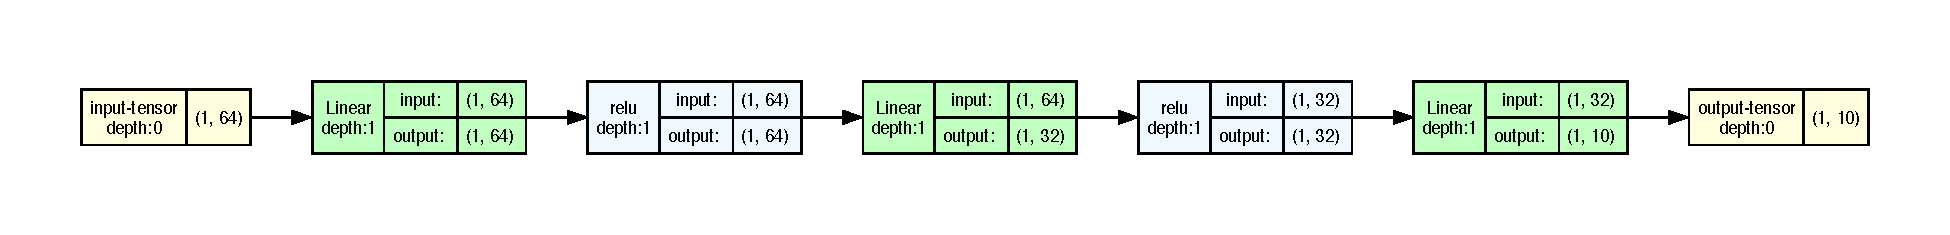
\includegraphics[width=\textwidth]{recursos_pdf/graficos/p2v_dist_model_H.pdf}
  \caption{Arquitectura del Modelo Base}
\end{figure}

La función de pérdida utilizada fue la Divergencia de Jensen-Shannon
(JSD) entre las distribuciones reales y predichas ponderando las 5
distribuciones a estimar. Se utilizó la implementación de Divergencia de
Kullback-Leibler de PyTorch \texttt{nn.KLDivLoss} en la implementación
del modulo \texttt{JSD} hayado en el foro de PyTorch(PyTorch Forums,
2022) y este luego se utilizó para la función de pérdida en el
entrenamiento del modelo.

\hypertarget{entrenamiento}{%
\subsection{Entrenamiento}\label{entrenamiento}}

Para entrenar el modelo, se utilizó el optimizador SGD (Stochastic
Gradient Descent) con una tasa de aprendizaje (lr) de 0.005, un momentum
de 0.9 y un weight decay de 0.0005 para prevenir el sobreajuste.

Además, se utilizó un scheduler de tasa de aprendizaje (scheduler) con
una estrategia de StepLR, que reduce la tasa de aprendizaje en un factor
de 0.1 cada 100 épocas. El entrenamiento se llevó a cabo durante un
máximo de 10,000 épocas, con un mecanismo de early stopping para detener
el entrenamiento si no se observaban mejoras en el rendimiento del
modelo en el conjunto de validación durante un número determinado de
épocas consecutivas.

\hypertarget{resultados-iniciales}{%
\subsection{Resultados iniciales}\label{resultados-iniciales}}

El modelo base se entrenó con los hiperparámetros y arquitectura
mencionados anteriormente, su entrenamiento finalizó en el epoch
\(2250\).

\begin{figure}
\centering
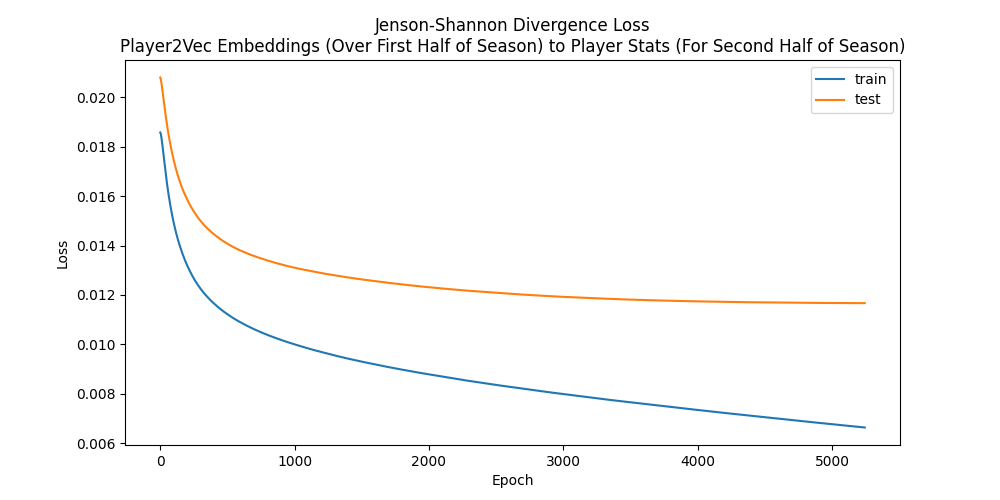
\includegraphics{recursos_pdf/graficos/p2v_dist_model_oos_190_for_graph_190_for_model_64_10000_0.005_StepLR.png}
\caption{Resultados del Modelo Base}
\end{figure}

\begin{table}
\caption{Resultados del Modelo Base}
\begin{tabular}{|c|c|c|}
\hline
\textbf{Métrica} & \textbf{Entrenamiento} & \textbf{Validación} \\
\hline
Loss & 0.01068 & 0.01505 \\
\hline
\end{tabular}
\end{table}

El modelo base obtuvo un rendimiento aceptable en el conjunto de
entrenamiento, con una pérdida de \(0.01068\), pero casi el 50\% mas en
el conjunto de validación, con una pérdida de \(0.01505\). Esto puede
ser un indicador de sobreajuste, por lo que se procedió a realizar un
proceso de tuning de hiperparámetros y arquitectura con validación
cruzada.

\hypertarget{tuning-de-hiperparuxe1metros-y-arquitectura-con-validaciuxf3n-cruzada}{%
\subsection{Tuning de Hiperparámetros y Arquitectura con Validación
Cruzada}\label{tuning-de-hiperparuxe1metros-y-arquitectura-con-validaciuxf3n-cruzada}}

Para mejorar el rendimiento del modelo, se realizó un proceso de tuning
de hiperparámetros y arquitectura con validación cruzada. Se evaluaron
distintas combinaciones de hiperparámetros y arquitecturas de red
neuronal, y se seleccionó la que mejor rendimiento presentó en el
conjunto de validación.

Del 80\% de los datos de entrenamiento, se separó un 20\% para
validación para hacer holdout CV.

\begin{table}
\caption{Split Datos de Entrenamiento, Validación y Test}
\begin{center}
\begin{tabular}{|c|c|}
\hline
\textbf{Conjunto} & \textbf{Tamaño} \\
\hline
Entrenamiento & 332 \\
Validación & 84 \\
Test & 105 \\
Total & 521 \\
\hline
\end{tabular}
\end{center}
\end{table}

Con la librería \texttt{Hyperopt} (Bergstra et al., 2015), se realizó
una búsqueda de hiperparámetros bayesina. Se evaluaron distintas
combinaciones de hiperparámetros, y se seleccionó la que mejor
rendimiento presentó en el conjunto de validación.

\subsection{Espacio de Hiperparámetros}

El espacio de hiperparámetros que se exploró fue el siguiente:

\begin{itemize}
    \item \textbf{Tasa de aprendizaje (lr)}: \{0.1, 0.01, 0.001\}
    \item \textbf{Momentum}: \{0.8, 0.9, 0.99\}
    \item \textbf{Weight decay}: \{0.0005, 0.0001\}
    \item \textbf{Optimizador}:
    \begin{itemize}
        \item SGD con momentum
        \item Adam
        \item AdamW
        \item RMSprop con momentum
    \end{itemize}
    \item \textbf{Scheduler}:
    \begin{itemize}
        \item StepLR con step\_size \{50, 100, 200\} y gamma \{0.1, 0.05, 0.01\}
        \item MultiStepLR con milestones \{50, 100, 200\} y gamma \{0.1, 0.05, 0.01\}
        \item ExponentialLR con gamma \{0.1, 0.05, 0.01\}
        \item CosineAnnealingLR con T\_max \{50, 100, 200\}
    \end{itemize}
    \item \textbf{Early stopping}: \{True\}
    \item \textbf{Early stopping window}: \{10, 20, 50, 100\}
\end{itemize}

Además se implementó una clase de Red Neuronal paramétrica para poder
explorar distintas arquitecturas de red neuronal.

\hypertarget{resultados-del-tuning-de-hiperparuxe1metros}{%
\subsection{Resultados del Tuning de
Hiperparámetros}\label{resultados-del-tuning-de-hiperparuxe1metros}}

La busqueda de hiperparámetros se realizó con 1000 iteraciones. La mejor
combinación de hiperparámetros y arquitectura de red neuronal encontrada
fue la siguiente:

\begin{itemize}
\tightlist
\item
  Tasa de aprendizaje: 0.01
\item
  Momentum: 0.9
\item
  Weight decay: 0.0001
\item
  Optimizador: \texttt{AdamW}
\item
  Scheduler: \texttt{CosineAnnealingLR}

  \begin{itemize}
  \tightlist
  \item
    T\_max: 200
  \end{itemize}
\item
  Arquitectura de red neuronal:

  \begin{itemize}
  \tightlist
  \item
    Activación: LeakyReLU
  \item
    Dropout: 0.3
  \item
    Número de capas: 8
  \item
    Tamaños de capas ocultas: (1024, 256, 64, 256, 256, 16, 32, 512)
  \end{itemize}
\end{itemize}

\begin{figure}[H]
  \centering
  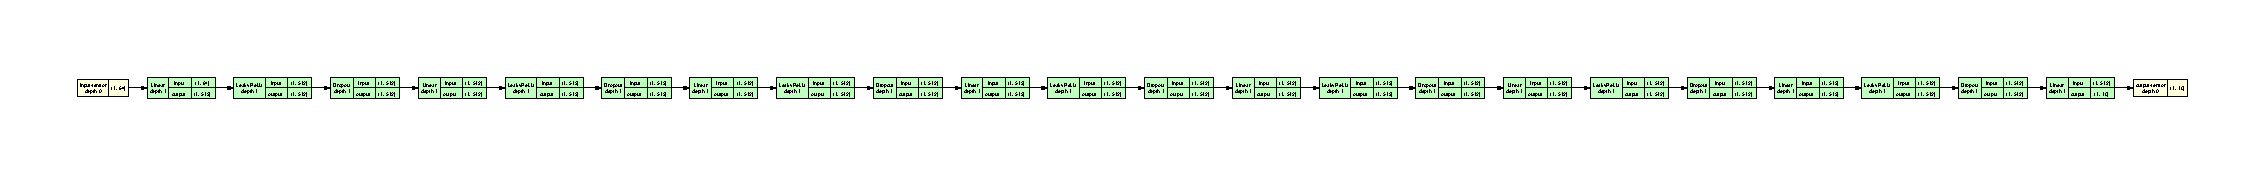
\includegraphics[width=\textwidth]{recursos_pdf/graficos/p2v_dist_model_tuned_H.pdf}
  \caption{Arquitectura del Modelo Tuned}
\end{figure}

(0.004966359119862318, 0.008916404098272324, 0.014493363909423351)

\begin{table}
\caption{Resultados del Modelo}
\label{tab:resultados_modelo_tuned}
\begin{center}
\begin{tabular}{lrrr}
\toprule
 & Train loss & Val loss & Test loss \\
\midrule
0 & 0.004966 & 0.008916 & 0.014493 \\
\bottomrule
\end{tabular}
\end{center}
\end{table}

El modelo final seleccionado obtuvo un rendimiento aceptable en el
conjunto de validación, con una pérdida de \(0.008916\), aún mejor que
la perdida de Train del modelo base. Se procedió a evaluar el modelo en
el conjunto de testeo y se obtuvo una pérdida de \(0.014493\).

\begin{figure}
\centering
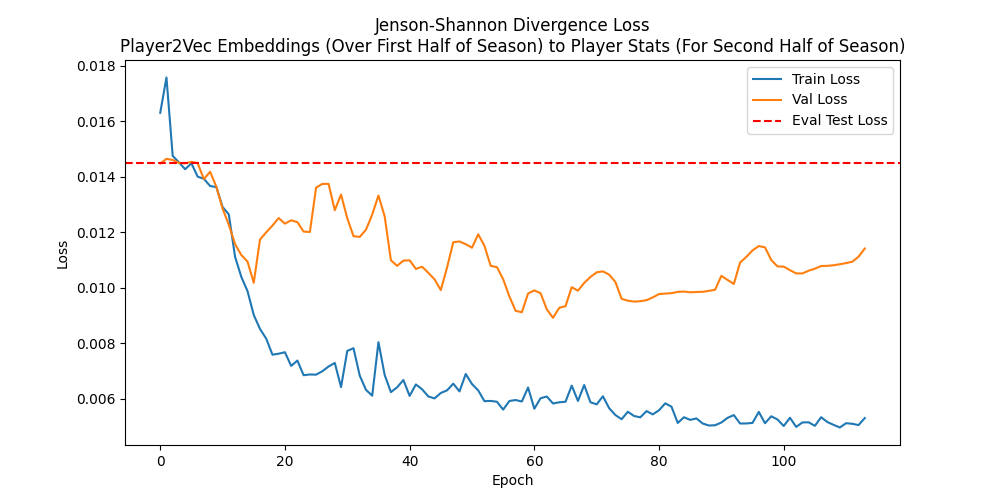
\includegraphics{recursos_pdf/graficos/p2v_dist_model_oos_190_for_graph_190_for_model_64_5000_0.01_CosineAnnealingLR_tuned_eval_test_loss.png}
\caption{Resultados del Modelo Tuned}
\end{figure}

El modelo resultante logró generalizar mejor, posiblemente estemos
presenciando un caso de overfitting del conjunto de validación, ya que
la pérdida en el conjunto de testeo es mayor que en el de validación,
sin embargo los resultados obtenidos son satisfactorios.

\hypertarget{hardware-y-tiempos-de-entrenamiento}{%
\subsection{Hardware y Tiempos de
Entrenamiento}\label{hardware-y-tiempos-de-entrenamiento}}

El entrenamiento del modelo base se realizó en una máquina con las
siguientes características:

Macbook Pro M1 2020 - Procesador: Apple M1 - Memoria RAM: 16 GB - GPU:
8-core GPU - 16-core Neural Engine - OS: macOS Sequoia 15.0.1 (24A348)

\begin{itemize}
\tightlist
\item
  Python 3.10.14
\item
  PyTorch 2.2.2 MPS (Metal Performance Shaders)
\end{itemize}

El entrenamiento del modelo final tomó tan solo 30 segundos a lo largo
de los 115 epochs que duró el entrenamiento por el mecanismo de early
stopping.

La busqueda de hiperparametros de 1000 iteraciones tomó al rededor de
7hs en la misma máquina.

\hypertarget{comparaciuxf3n-contra-priors}{%
\subsection{Comparación contra
priors}\label{comparaciuxf3n-contra-priors}}

Para evaluar la capacidad predictiva de nuestro modelo, comparamos los
resultados obtenidos con los priors de las distribuciones de ratios de
transición de los jugadores. Los priors se obtuvieron a partir de las
distribuciones de ratios de transición de los jugadores en la primera
mitad de la temporada 2012/13 de la EPL.

Asumiendo que las distribuciones de ratios de transición de los
jugadores en la segunda mitad de la temporada son similares a las de la
primera mitad, evaluamos su capacidad predictiva con la misma función de
pérdida JSD ponderada, obteniendo los siguientes resultados:

\begin{table}
\caption{Resultados del Modelo vs Priors}
\begin{center}
\begin{tabular}{|c|c|c|}
\hline
\textbf{Modelo} & \textbf{Priors} \\
\hline
\colorbox{yellow}{$0.014493$} & 0.0353 \\
\hline
\end{tabular}
\end{center}
\end{table}

Por lo que se puede observar, el modelo logra una mejora significativa
en la capacidad predictiva de las distribuciones de ratios de transición
de los jugadores en comparación con asumir igualdad de distribuciones
entre las dos mitades de la temporada. En concreto, nuestro modelo logra
reducir la pérdida en un \(\sim 58.94\%\) en comparación con los priors.

\newpage

\hypertarget{validaciuxf3n-del-modelo}{%
\section{\texorpdfstring{\textbf{Validación del Modelo de
Distribuciones}}{Validación del Modelo de Distribuciones}}\label{validaciuxf3n-del-modelo}}

Para evaluar la capacidad de nuestro modelo en escenarios reales,
desarrollamos un caso de estudio basado en las transferencias más
importantes en términos de precio y relevancia mediática de los próximos
dos mercados de fichajes dentro de la Premier League. Nos limitamos a
transferencias internas de esta liga debido a la falta de datos
disponibles sobre otras competiciones. Este ejercicio busca medir qué
tan bien nuestras métricas y simulaciones pueden justificar o
desaconsejar dichas transferencias en función de su impacto en el
rendimiento del equipo.

En este apartado, profundizaremos en el análisis de dos casos
específicos: la transferencia de Danny Welbeck al Arsenal y la de James
Milner al Liverpool. Finalmente, presentaremos una tabla resumen con
seis transferencias clave, acompañadas de las recomendaciones de nuestro
modelo.

Para comparar las distribuciones de PSL de los jugadores involucrados en
las transferencias, utilizamos las métricas de comparación de
distribuciones presentadas anteriormente: comparación de momentos,
dominancia probabilística y dominancia estocástica.

\hypertarget{caso-de-estudio-1-danny-welbeck-al-arsenal}{%
\subsection{Caso de Estudio 1: Danny Welbeck al
Arsenal}\label{caso-de-estudio-1-danny-welbeck-al-arsenal}}

Para analizar la transferencia de Danny Welbeck (delantero) al Arsenal,
evaluamos el impacto en el PSL del equipo simulando su inclusión en
lugar de los principales delanteros titulares. Para ello, consideramos
dos escenarios: en el primero, Welbeck reemplaza a Theo Walcott creando
la formación \(L_{AR1}^{\text{Welbeck}}\) cuya distribución es
\(X_{L_{AR1}^{\text{Welbeck}}} \sim \hat{f}^{1000}_{PSL}(L_{AR1}^{\text{Welbeck}})\).
Y en el segundo, a Olivier Giroud creando la formación
\(L_{AR2}^{\text{Welbeck}}\) cuya distribución es
\(X_{L_{AR2}^{\text{Welbeck}}} \sim \hat{f}^{1000}_{PSL}(L_{AR2}^{\text{Welbeck}})\).

Los resultados obtenidos son los siguientes:

\begin{figure}
  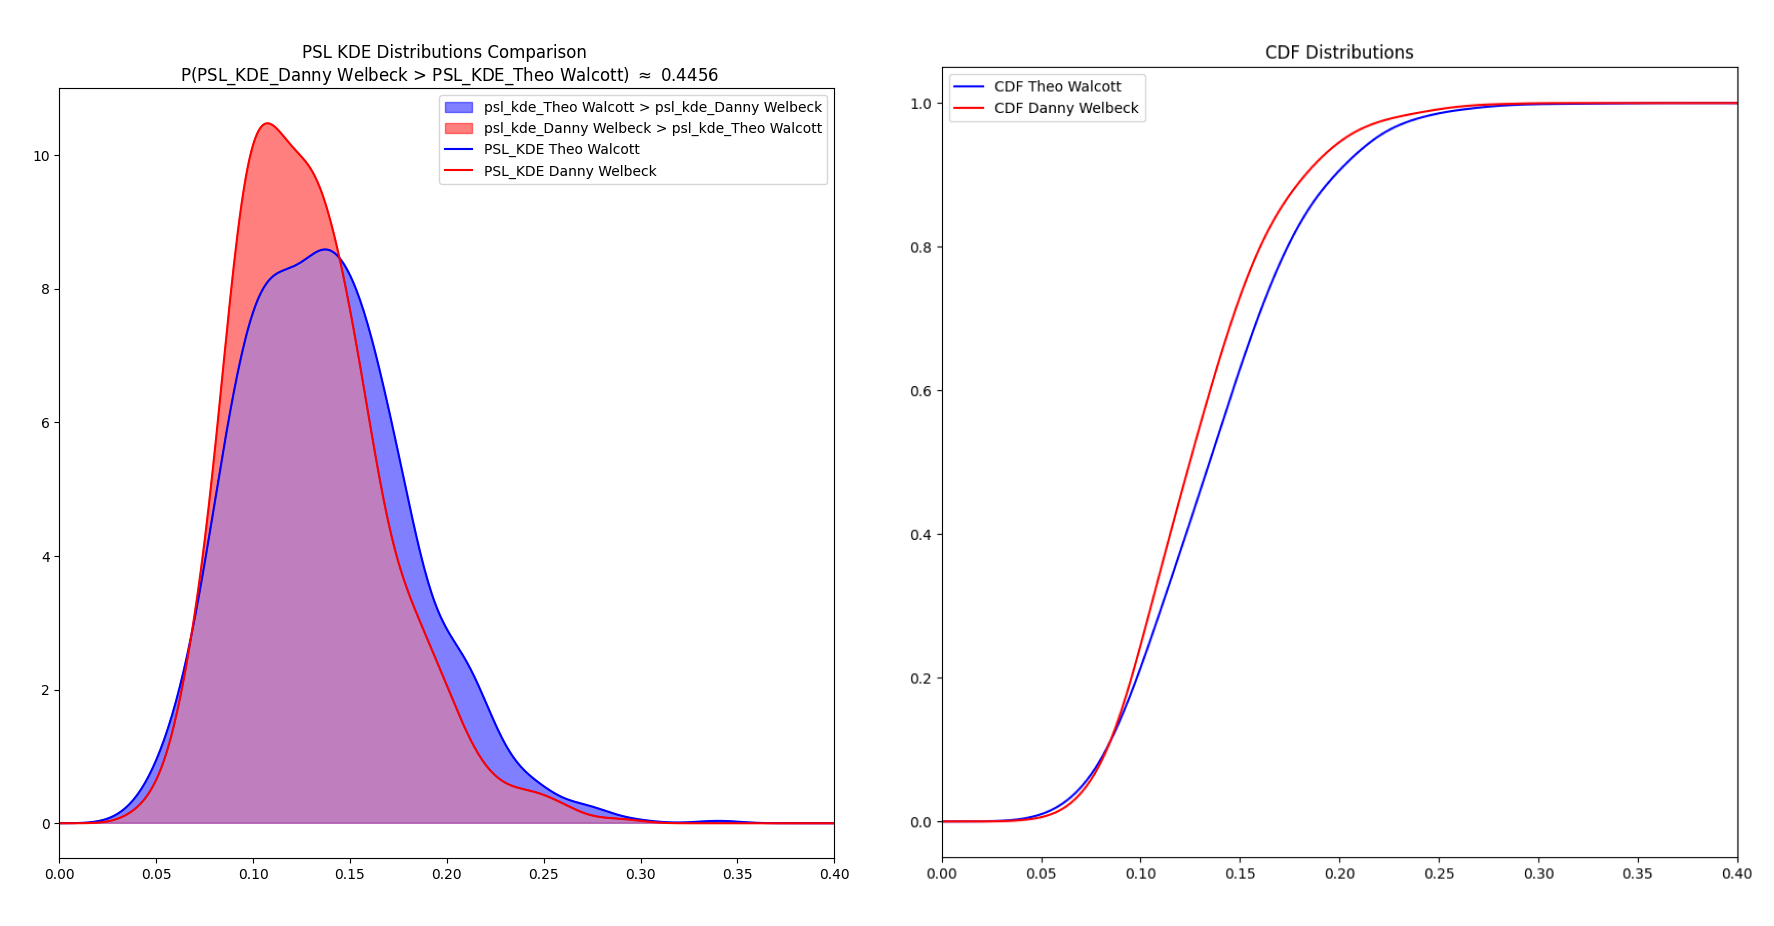
\includegraphics{recursos_pdf/graficos/Welbeck_Walcott.png}
    \caption{Comparación de CDFs y PDFs de Welbeck y Walcott}
\end{figure}

\begin{table}
\caption{Comparación de momentos de $X_{L_{AR1}^{\text{Welbeck}}}$ y $X_{L_{AR1}}$}
\label{tab:comparacion_momentos_psl_Welbeck_Walcott}
\begin{center}
\begin{tabular}{llllll}
\toprule
Jugador & Media & Varianza & Desvio Estándar & Skewness & Kurtosis \\
\midrule
Theo Walcott  &  0.137735 &  0.043914 &         0.001928 &  0.547502 &  0.421810 \\
Danny Welbeck &  0.129325 &  0.038815 &         0.001507 &  0.761120 &  0.773602 \\
\bottomrule
\end{tabular}
\end{center}
\end{table}

\begin{figure}
  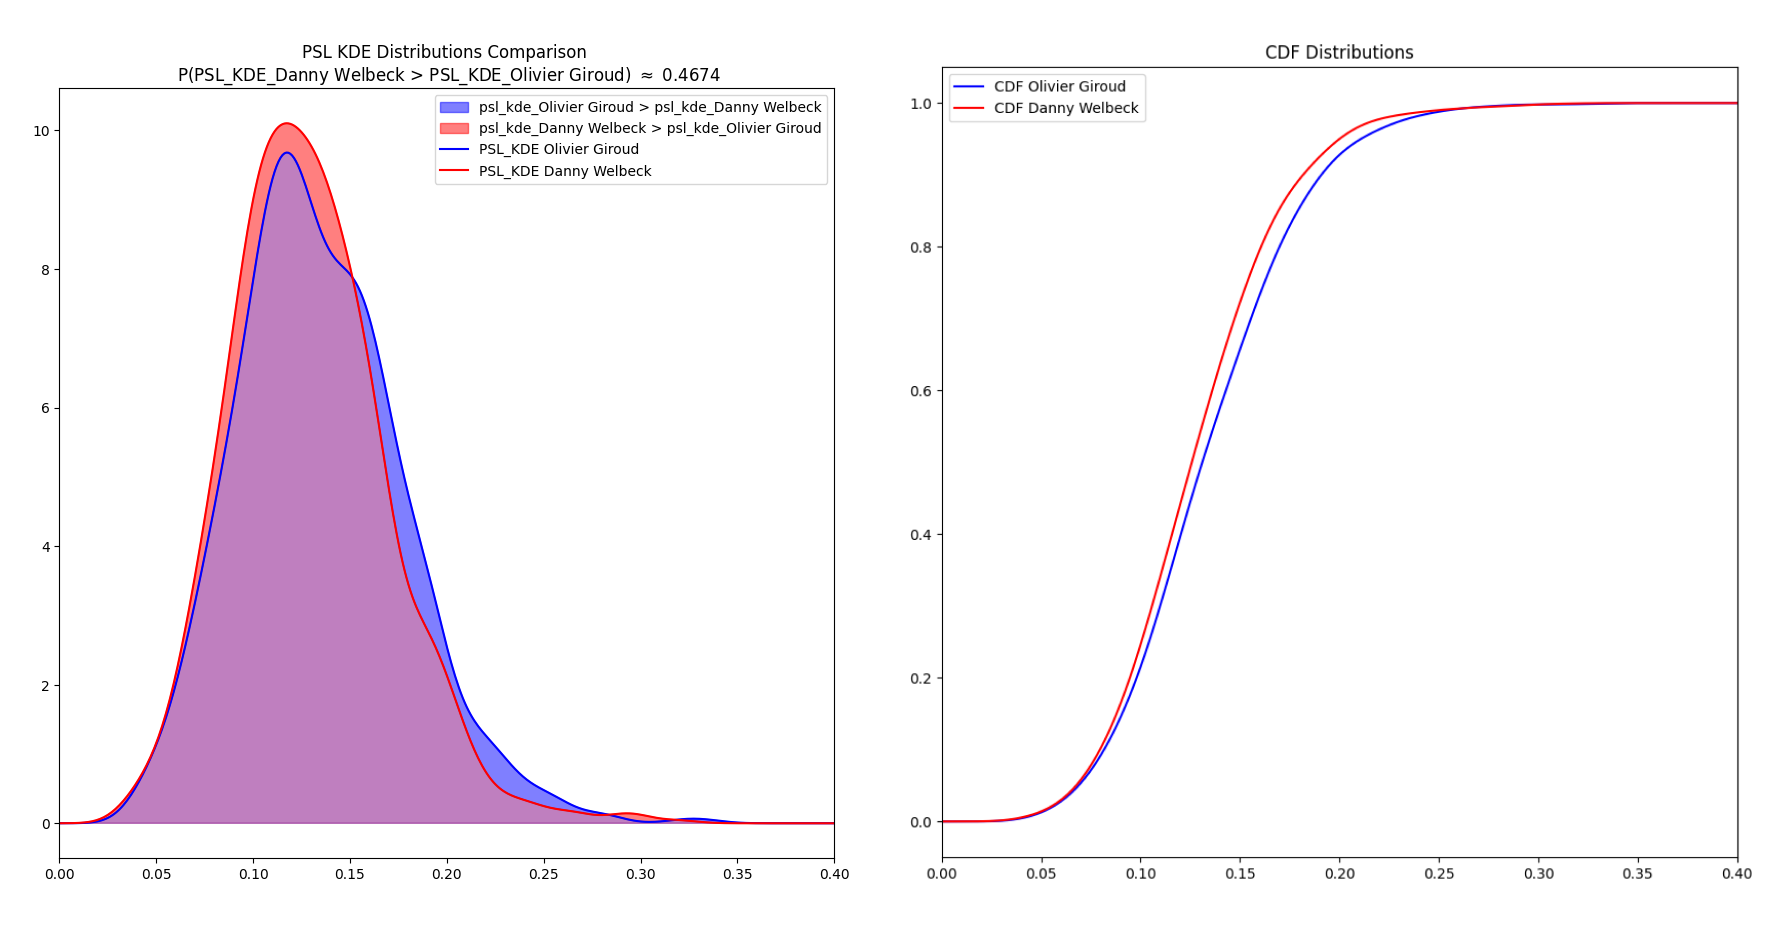
\includegraphics{recursos_pdf/graficos/Welbeck_Giroud.png}
    \caption{Comparación de CDFs y PDFs de Welbeck y Giroud}
\end{figure}

\begin{table}
\caption{Comparación de momentos de $X_{L_{AR2}^{\text{Welbeck}}}$ y $X_{L_{AR2}}$}
\label{tab:comparacion_momentos_psl_Welbeck_Giroud}
\begin{center}
\begin{tabular}{llllll}
\toprule
Jugador & Media & Varianza & Desvio Estándar & Skewness & Kurtosis \\
\midrule
Olivier Giroud &  0.134801 &  0.042535 &         0.001809 &  0.587343 &  0.777267 \\
Danny Welbeck  &  0.128931 &  0.040130 &         0.001610 &  0.700550 &  1.325063 \\
\bottomrule
\end{tabular}
\end{center}
\end{table}

Como se puede observar, la distribución de la formación con Walcott,
\(X_{L_{AR1}}\), presenta una mayor media en PSL en comparación con
\(X_{L_{AR1}^{\text{Welbeck}}}\). Además, al observar ``a ojo'' la PDF
de \(X_{L_{AR1}}\), notamos un mayor sesgo hacia la derecha, lo que
indica que la formación con Walcott posee un PSL superior al de la
formación con Welbeck en la mayoría de los casos.

Dado que \(P(X_{L_{AR1}^{\text{Welbeck}}} > X_{L_{AR1}}) = 0.44\), se
sigue que \(P(X_{L_{AR1}} > X_{L_{AR1}^{\text{Welbeck}}}) = 0.56\), lo
cual indica que la formación con Walcott tiene dominancia probabilística
sobre la formación con Welbeck.

Asimismo, podemos concluir que la formación con Walcott domina
estocásticamente a la formación con Welbeck, ya que la CDF de
\(X_{L_{AR1}}\) es mayor que la de \(X_{L_{AR1}^{\text{Welbeck}}}\) en
todos los puntos a partir del umbral de 0.07.

Todas estas métricas se repiten a favor de la formación con Giroud,
\(X_{L_{AR2}}\), en comparación con \(X_{L_{AR2}^{\text{Welbeck}}}\).

Por lo tanto, podemos concluir que, según nuestro modelo, la
transferencia de Danny Welbeck al Arsenal no es recomendable porque su
inclusión en lugar de Theo Walcott o Olivier Giroud disminuiría el PSL
del equipo y empeoraria la performance del mismo.

\newpage

\hypertarget{caso-de-estudio-2-james-milner-al-liverpool}{%
\subsection{Caso de Estudio 2: James Milner al
Liverpool}\label{caso-de-estudio-2-james-milner-al-liverpool}}

Para analizar la transferencia de James Milner(Mediocampista) utilizamos
la misma metodología que en el caso anterior. Evaluamos el impacto en el
PSL del equipo simulando su inclusión en lugar de los principales
mediocampistas titulares. Para ello, consideramos dos escenarios: en el
primero, Milner reemplaza a Steven Gerrard creando la formación
\(L_{LIV1}^{\text{Milner}}\) cuya distribución es
\(X_{L_{LIV1}^{\text{Milner}}} \sim \hat{f}^{1000}_{PSL}(L_{LIV1}^{\text{Milner}})\).
Y en el segundo, a Stewart Downing creando la formación
\(L_{LIV2}^{\text{Milner}}\) cuya distribución es
\(X_{L_{LIV2}^{\text{Milner}}} \sim \hat{f}^{1000}_{PSL}(L_{LIV2}^{\text{Milner}})\).

Los resultados obtenidos luego de la simulación son los siguientes:

\begin{figure}
  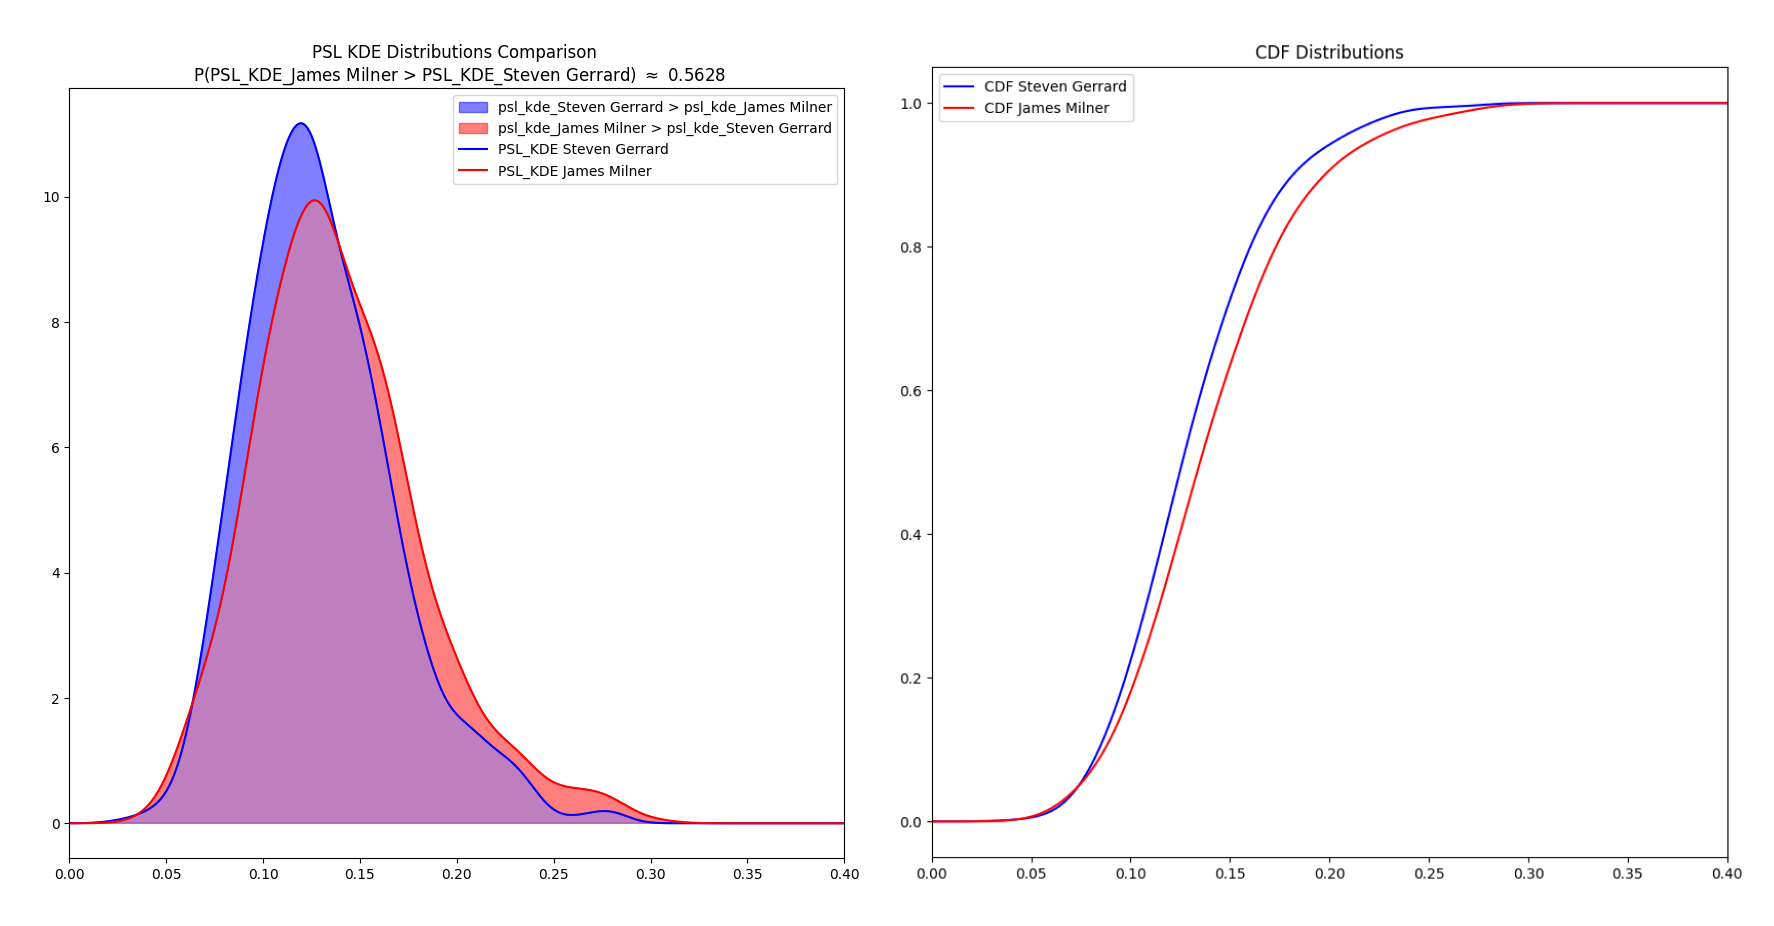
\includegraphics{recursos_pdf/graficos/Milner_Gerrard.png}
    \caption{Comparación de CDFs y PDFs de Milner y Gerrard}
\end{figure}

\begin{table}
\caption{Comparación de momentos de $X_{L_{LIV1}^{\text{Milner}}}$ y $X_{L_{LIV1}}$}
\label{tab:comparacion_momentos_psl_Milner_Gerrard}
\begin{center}
\begin{tabular}{llllll}
\toprule
Jugador & Media & Varianza & Desvio Estándar & Skewness & Kurtosis \\
\midrule
Steven Gerrard &  0.130349 &  0.038290 &         0.001466 &  0.748219 &  0.862186 \\
James Milner   &  0.139559 &  0.043333 &         0.001878 &  0.703642 &  0.712261 \\
\bottomrule
\end{tabular}
\end{center}
\end{table}

\begin{figure}
  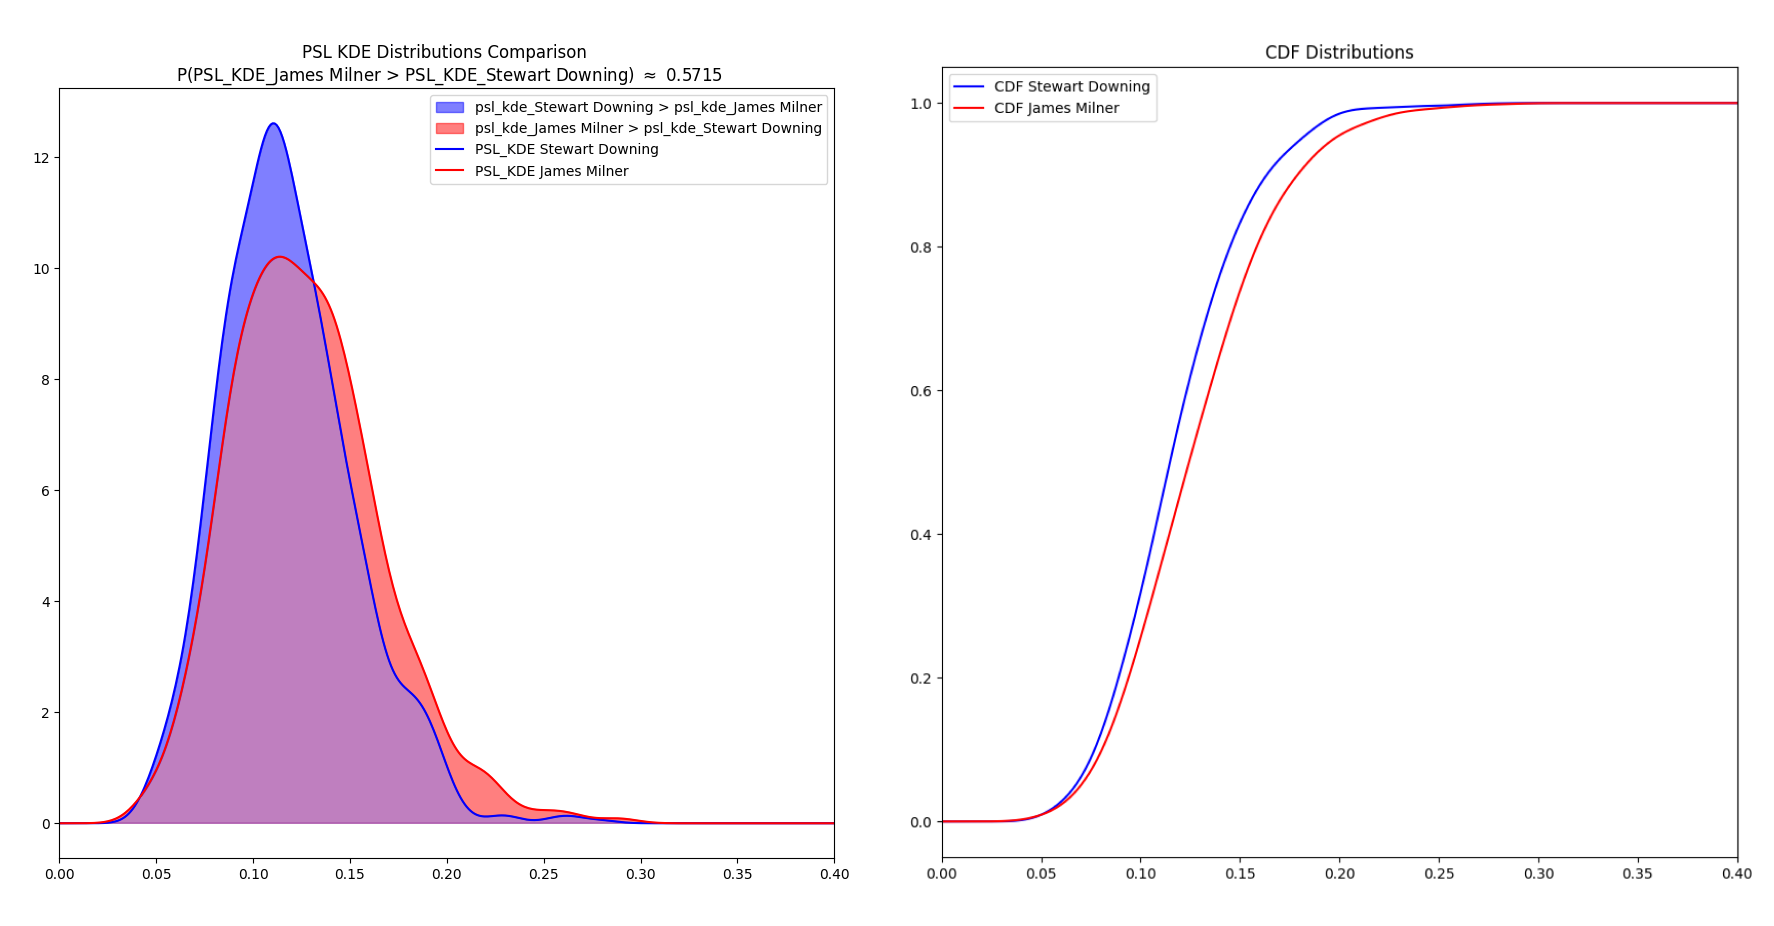
\includegraphics{recursos_pdf/graficos/Milner_Downing.png}
    \caption{Comparación de CDFs y PDFs de Milner y Downing}
\end{figure}

\begin{table}
\caption{Comparación de momentos de $X_{L_{LIV2}^{\text{Milner}}}$ y $X_{L_{LIV2}}$}
\label{tab:comparacion_momentos_psl_Milner_Downing}
\begin{center}
\begin{tabular}{llllll}
\toprule
Jugador & Media & Varianza & Desvio Estándar & Skewness & Kurtosis \\
\midrule
Stewart Downing &  0.117987 &  0.033518 &         0.001123 &  0.696171 &  1.087000 \\
James Milner    &  0.127622 &  0.038303 &         0.001467 &  0.651483 &  0.768572 \\
\bottomrule
\end{tabular}
\end{center}
\end{table}

Como se puede observar, ambas distribuciones con Milner,
\(X_{L_{LIV1}^{\text{Milner}}}\) y \(X_{L_{LIV2}^{\text{Milner}}}\),
presentan una mayor media en PSL en comparación con \(X_{L_{LIV1}}\) y
\(X_{L_{LIV2}}\) respectivamente. Además, al observar ``a ojo'' las PDFs
de \(X_{L_{LIV1}^{\text{Milner}}}\) y \(X_{L_{LIV2}^{\text{Milner}}}\),
notamos un mayor sesgo hacia la derecha que las originales, lo que
indica que las formaciones con Milner poseen un PSL superior en la
mayoría de los casos.

Dado que \(P(X_{L_{LIV1}^{\text{Milner}}} > X_{L_{LIV1}}) = 0.56\) y
\(P(X_{L_{LIV2}} > X_{L_{LIV2}^{\text{Milner}}}) = 0.57\), implica que
las formaciones con Milner tienen dominancia probabilística sobre las
formaciones originales.

También notamos que las CDFs de \(X_{L_{LIV1}^{\text{Milner}}}\) y
\(X_{L_{LIV2}^{\text{Milner}}}\) son mayores que las originales en todos
los puntos a partir del umbral de 0.06, lo que indica que las
formaciones con Milner dominan estocásticamente a las formaciones
originales.

Por lo tanto, podemos concluir que, según nuestro modelo, la
transferencia de James Milner al Liverpool es recomendable porque su
inclusión en lugar de Steven Gerrard o Stewart Downing mejoraría el PSL
del equipo y aumentaría la performance del mismo.

\hypertarget{recomendaciones-de-transferencias-clave}{%
\subsection{Recomendaciones de Transferencias
Clave}\label{recomendaciones-de-transferencias-clave}}

En la tabla a continuación se presentan las seis transferencias más
importantes dentro de la Premier League en la temporada 13/14, evaluadas
según nuestro modelo. Cada transferencia fue analizada utilizando las
distribuciones de PSL del jugador y simulando su impacto en el
rendimiento del equipo destino. Las recomendaciones se clasificaron en:

\begin{itemize}
\item
  \textbf{Recomendable}: La transferencia mejora el PSL del equipo
  destino.
\item
  \textbf{No Recomendable}: La transferencia empeora el PSL del equipo
  destino.
\item
  \textbf{Indeciso}: La transferencia no tiene un impacto significativo
  en el PSL del equipo destino.
\end{itemize}

\begin{table}
\caption{Recomendaciones de Transferencias Clave}
\label{tab:recomendaciones_transferencias}
\begin{center}
\begin{tabular}{lllll}
\toprule
Jugador & Posición & Equipo Origen & Equipo Destino & Recomedación \\
\midrule
James Milner & Mediocampista & Manchester City & Liverpool & Recomendable \\
Andros Townsend & Mediocampista & Tottenham & Newcastle & Recomendable \\
Juan Mata & Mediocampista & Chelsea & Manchester United & Recomendable \\
Romelu Lukaku & Delantero & Chelsea & Everton & Indeciso \\
Ryan Bertrand & Defensor & Chelsea & Southampton & No Recomendable \\
Danny Welbeck & Delantero & Manchester United & Arsenal & No Recomendable \\
\bottomrule
\end{tabular}
\end{center}
\end{table}

\hypertarget{resultados}{%
\section{\texorpdfstring{\textbf{Resultados}}{Resultados}}\label{resultados}}

\hypertarget{discusiuxf3n}{%
\section{\texorpdfstring{\textbf{Discusión}}{Discusión}}\label{discusiuxf3n}}

\hypertarget{conclusiones-recomendaciones-conclusiones--recomendaciones}{%
\section{\texorpdfstring{\textbf{Conclusiones \& Recomendaciones}
\{\#conclusiones-\&-recomendaciones\}}{Conclusiones \& Recomendaciones \{\#conclusiones-\&-recomendaciones\}}}\label{conclusiones-recomendaciones-conclusiones--recomendaciones}}

\newpage

\hypertarget{referencias-bibliogruxe1ficas}{%
\section{\texorpdfstring{\textbf{Referencias
bibliográficas}}{Referencias bibliográficas}}\label{referencias-bibliogruxe1ficas}}

\hypertarget{refs}{}
\begin{CSLReferences}{1}{0}
\leavevmode\vadjust pre{\hypertarget{ref-bawa_1982_stochastic}{}}%
Bawa, V. S. (1982). Stochastic dominance: A research bibliography.
\emph{Management Science}, \emph{28}, 698--712.
\url{https://doi.org/10.1287/mnsc.28.6.698}

\leavevmode\vadjust pre{\hypertarget{ref-bergstra_2015_hyperopt}{}}%
Bergstra, J., Komer, B., Eliasmith, C., Yamins, D., \& Cox, D. D.
(2015). Hyperopt: A python library for model selection and
hyperparameter optimization. \emph{Computational Science \& Discovery},
\emph{8}, 014008. \url{https://doi.org/10.1088/1749-4699/8/1/014008}

\leavevmode\vadjust pre{\hypertarget{ref-grover_2016_node2vec}{}}%
Grover, A., \& Leskovec, J. (2016). \emph{node2vec: Scalable feature
learning for networks}. arXiv.org.
\url{https://arxiv.org/abs/1607.00653}

\leavevmode\vadjust pre{\hypertarget{ref-gustavo_decision}{}}%
Gustavo, V. (n.d.-b). \emph{Decision under risk - module IV - NYU stern
- master of science in business analytics}.

\leavevmode\vadjust pre{\hypertarget{ref-gustavo_NYU}{}}%
Gustavo, V. (n.d.-a). \emph{Decision under risk - module IV - NYU stern
- master of science in business analytics}.

\leavevmode\vadjust pre{\hypertarget{ref-huang_soccer_networks}{}}%
Huang, E., Segarra, S., Gallino, S., \& Ribeiro, A. (n.d.). \emph{How to
find the right player for your soccer team?}

\leavevmode\vadjust pre{\hypertarget{ref-mikolov_2013_word2vec}{}}%
Mikolov, T., Chen, K., Corrado, G., \& Dean, J. (2013). \emph{Efficient
estimation of word representations in vector space}. arXiv.org.
\url{https://arxiv.org/abs/1301.3781}

\leavevmode\vadjust pre{\hypertarget{ref-alexneakamenipytorchforums_2022_jensen}{}}%
PyTorch Forums, A. N. K. -. (2022). \emph{Jensen shannon divergence}.
PyTorch Forums.
\url{https://discuss.pytorch.org/t/jensen-shannon-divergence/2626/13}

\leavevmode\vadjust pre{\hypertarget{ref-rahimian_2023}{}}%
Rahimian, P., Van Haaren, J., \& Toka, L. (2023). Towards maximizing
expected possession outcome in soccer. \emph{International Journal of
Sports Science \& Coaching}, 174795412311544.
\url{https://doi.org/10.1177/17479541231154494}

\leavevmode\vadjust pre{\hypertarget{ref-tippett_2019_the}{}}%
Tippett, J. (2019). \emph{The expected goals philosophy: A game-changing
way of analysing football}. Independently Published.

\end{CSLReferences}

\hypertarget{apuxe9ndices}{%
\section{\texorpdfstring{\textbf{Apéndices: Tablas, figuras,
anexos}}{Apéndices: Tablas, figuras, anexos}}\label{apuxe9ndices}}

\listoffigures
\listoftables
\tocfile{Índice de Algoritmos}{loa}

\end{document}
